 \documentclass[a4paper,12pt]{report}
  \pagestyle{plain}
  \usepackage{latexsym}      %symboly
  \usepackage{graphicx}
  \usepackage{amsmath}
  \usepackage{amsfonts}
  \usepackage{amsthm}
  \usepackage{epstopdf} %pokud pouzivam .eps obrazky, ale chci prekladat pdflatexem 
  \usepackage[czech]{babel}
  \usepackage[utf8]{inputenc} %pro vstupní kódování  
  %\usepackage[utf8x]{inputenc} %pro vstupní kódování  umožní více jazyků, ale má jiné problémy
  \usepackage[T1]{fontenc} %pro výstupní kódování fontů (pro UTF8), aby fungovalo dělení slov s diakritikou a vyhledávání slov s diakritikou
  %\usepackage[IL2]{fontenc} %pro výstupní kódování fontů (pro latin2, ale obsahuje víc fontů než [T1]), aby fungovalo dělení slov s diakritikou a vyhledávání slov s diakritikou
  \usepackage{lmodern} %balíček zavádějící fonty Latin Modern. Bez něj se použijí starší, tzv. EC fonty, jejichž typografická úroveň je v případě češtiny nízká
  %\usepackage{palatino} % Font Palatino alternativa k \usepackage{lmodern} 
  \usepackage{comment}
  \usepackage{xcolor}

\usepackage{url}  %kvuli vkladani URL adres do bibtexu ale asi jen ve stylu CZECHISO
\DeclareUrlCommand\url{\def\UrlLeft{<}\def\UrlRight{>} \urlstyle{tt}}
  
%\renewcommand{\figurename}{Fig.}
  \usepackage{phdthesis}
  \usepackage{psfrag}
%  \newtheorem{definice}{Definition}
  \usepackage{hyperref} % klikatelne odkazy v textu
  \hypersetup{
      colorlinks   = true, %Colours links instead of ugly boxes
      urlcolor     = blue, %Colour for external hyperlinks
      linkcolor    = red, %Colour of internal links
      citecolor   = red, %Colour of citations
      unicode=true % zajistí správné fungování háčků a čárek (češtiny) v PDF obsahu
    }
  \date{\today}
  \usepackage{minibox}
  \usepackage{pdfpages}
%
%
\vfuzz10pt % Don't report over-full v-boxes if over-edge is small
\hfuzz10pt
%
%
%\newtheorem{theorem}{Theorem}[chapter]
%\newtheorem{definition}{Definition}[chapter]
%\newtheorem{example}{Example}[chapter]
\DeclareMathOperator{\limean}{l.i.m.}   %limit in the mean se stane operatorem
\DeclareMathOperator{\argmax}{argmax}   %stejne tak argmin a argmax
\DeclareMathOperator{\argmin}{argmin}
%
%

\newtheorem{veta}{Věta} 
\newtheorem{lemma}[veta]{Lemma}
\newtheorem{dusledek}[veta]{Důsledek}
\theoremstyle{definition} \newtheorem{definice}[veta]{Definice}
\newtheorem{priklad}{Příklad}
\theoremstyle{remark}
\newtheorem*{poznamka}{Poznámka}
\newtheorem*{reseni}{Řešení}  

%\newcommand{\uv}[1]{\quotedblbase #1\textquotedblleft} %makro pro české uvozovky


\newcommand{\specialcell}[2][c]{%
\begin{tabular}[#1]{@{}l@{}}#2\end{tabular}}

%\usepackage{encxvlna} %při překladu automaticky uvažuje nezlomitelné mezery dle pravidel češtiny (nahrazuje program vlna.exe)

\begin{document}
\titlepage
\vspace*{-2.4cm}
\begin{center}
\textsc{\Large{Masarykova Univerzita}} \\
\large{Přírodovědecká fakulta} \\
\large{Ústav matematiky a statistiky}
\end{center}
\vspace{7.11cm}
%
\begin{center}
\textsc{\Large{DISERTAČNÍ PRÁCE}}
\end{center}
%
\vspace{11.39cm}
%
\begin{center}
\begin{tabular}{l  r}
 \Large{Brno 2016} \qquad\qquad\qquad\qquad \qquad\qquad & \Large{Lenka Křivánková}
\end{tabular}
\end{center}

\titlepage
\begin{center}
\textsc{\Large{Masarykova Univerzita}} \\
\textsc{\Large{Přírodovědecká fakulta}} \\
\textsc{\large{Ústav matematiky a statistiky}}
\end{center}\quad \\
%
\begin{center}

\includegraphics[width=5cm]{IMG/sci-logo.pdf}
\end{center}\quad \\
%
\begin{center}
\textbf{\Large{Stochastické metody analýzy ekonomických dat}} \\ \quad \\
\textsc{\large{Disertační práce}}
\end{center} \quad \\\\\\\\\\\\\\\\\\\\\\\\\\ \\
\begin{center}
\large{
\begin{tabular}{l  r}
\Large{Brno 2016} \qquad\qquad\qquad\qquad \qquad\qquad & \Large{Lenka Křivánková}
\end{tabular}
}
\end{center} \quad
%
%\begin{center}
%\large{Brno 2009}
%\end{center}
%\begin{center}
%\verb=   (\(\=\\
%\verb=  (._. )=\\
%\verb=(')(')_)o=
%\end{center}

\normalsize



\chapter*{Bibliografický záznam}\addcontentsline{toc}{chapter}{Bibliografický záznam}
\setcounter{page}{1}
\pagenumbering{roman}
%\thispagestyle{empty}

\begin{tabular}{p{3.9cm}  p{9.1cm}}
\textbf{Autor:} & Mgr. Lenka Křivánková \\
\textbf{Název:} & Stochastické metody analýzy ekonomických dat \\
\textbf{Školitel:} & doc. RNDr. Martin Kolář, Ph.D.  \\
\textbf{Studijní program:} & Matematika \\
\textbf{Obor:} & Pravděpodobnost, statistika a matematické modelování \\
\textbf{Rok obhajoby:} & 2016 \\
\textbf{Klíčová slova:} & Stochastické procesy, \\
\end{tabular}
\\\\\\\\\\

\begin{flushright} {{\Huge Bibliographic entry}} \vspace{38pt} \end{flushright}
%\addcontentsline{toc}{chapter}{Bibliographic entry}

\hspace{-0.7cm}
\begin{tabular}{p{3.9cm}  p{9.1cm}}
\textbf{Author:} & Mgr. Lenka Křivánková \\
\textbf{Title:} & Stochastic methods in analysis of economic data \\
\textbf{Supervisor:} & doc. RNDr. Martin Kolář, Ph.D.  \\
\textbf{Study programme:} & Mathematics \\
\textbf{Study field:} & Probability, statistics and mathematical modeling \\
\textbf{Year of defence:} & 2016 \\
\textbf{Keywords:} & Stochastic processes, \\
\end{tabular}
\newpage
\pagestyle{empty}
\null
\vfill
\begin{center}
\copyright \quad Lenka Křivánková, Masarykova Univerzita, 2016
\end{center}

\chapter*{Poděkování}\addcontentsline{toc}{chapter}{Poděkování}
%\thispagestyle{empty}
\pagestyle{plain}
Na tomto místě
\\

Brno, Červenec 2016
\\

Lenka Křivánková

\chapter*{Abstrakt}\addcontentsline{toc}{chapter}{Abstrakt}
%\thispagestyle{empty}
V první části práce jsou uvedeny základní matematické pojmy použité v dalších částech textu. 
\\\\\\\\\\

\begin{flushright} {{\Huge Abstract}} \vspace{38pt} \end{flushright}
%\addcontentsline{toc}{chapter}{Abstract}
In the first part of the work, some basic mathematical methods employed in this thesis are recalled. 

\tableofcontents \addcontentsline{toc}{chapter}{Obsah}

\chapter*{Seznam použitého značení}\addcontentsline{toc}{chapter}{Seznam použitého značení} 
%\hspace{-0.7cm}
%\begin{tabular}{r  l}
%$\mathsf{E}X$ & Expected value of random variable $X$ \\
%$\mathsf{var}X$ & Dispersion, resp. variance of random variable X \\
%\end{tabular}

\normalsize
\textbf{Prostory a matice}\\\\
%  \begin{table}[h]
   \begin{tabular}{p{4cm} p{9.3cm}}
   $\mathbb{R}$                              &   jednorozměrný Eukleidovský prostor \\
   $\mathbb{R}^n$                              &     $n$-rozměrný Eukleidovský prostor \\
   $\mathbb{R}^+$                              &     množina všech kladných čísel \\
   $\boldsymbol{x}=(x_1,\ldots,x_n)^\mathrm{T}$             &    $n$-rozměrný reálný vektor \\
    $\boldsymbol{1}$                           &   vektor jedniček\\
   $\mathbf{I}_n$                              &    jednotková matice řádu $n$ \\
   $\mathbf{A}^\mathrm{T}$                              &   transponovaná matice vzhledem k matici $\mathbf{A}$\\
   \end{tabular}\\\\\\
% \end{table}
%
%
\textbf{Pravděpodobnost}\\\\
%  \begin{table}[h]
   \begin{tabular}{p{4cm} p{9.3cm}}
   $\omega$				        & elementární jev\\
   $\Omega$                                          &   základní prostor, množina všech elementárních jevů \\
   $\mathsf{Pr}(A)$                               &  pravděpodobnost jevu $A$ \\
   $(\Omega,\mathcal{A}, \mathsf{Pr})$                         &   pravděpodobnostní prostor \\
   \end{tabular}\\\\\\
%
%  \end{table}
%
%
\textbf{Náhodné veličiny}\\\\
%  \begin{table}[h]
   \begin{tabular}{p{4cm} p{9.3cm}}
   $X$; $X(\omega)$                                                 &   náhodná veličina \\
   $f(x)$; $f_X(x)$                                               &   hustota pravděpodobnosti náhodné veličiny $X$ \\ %probability density of the random variable $X$ \\
   $F(x)$; $F_X(x)$				 &  distribuční funkce náhodné veličiny $X$ \\
%   $f(x; \theta)$                                    &   probability density function of random variable $X$ with distribution dependent on scalar parameter $\theta$ \\
%   $f(x,t)$                                          &    probability density of random process $X(t)$ at fixed time $t$ \\
%   $f(x,t | x_0, t_0)$                               &    probability density of random process $X(t)$ at fixed time $t$ conditioned by its state $x_0$ at time $t_0$ \\
   $X\sim \mathcal{L}(\boldsymbol{\theta})$                                &   náhodná veličina $X$ mající rozdělením pravděpodobnosti $\mathcal{L}$ s parametry  $\boldsymbol{\theta}=(\theta_1,\ldots,\theta_n)$ \\ %random variable $X$ having general probability distribution $\mathcal{L}$\\
   $\mathsf{E}(X)$;  $\mathsf{E}X$                         	      &   střední hodnota náhodné veličiny $X$ \\
   $\mathsf{D}(X)$;  $\mathsf{D}X$                       	      &   rozptyl náhodné veličiny $X$ \\
   $\mathsf{C}(X_i,X_j)$             		      &   kovariance náhodných veličin $X_i$ a $X_j$\\
   $\mathsf{N}(\mu, \sigma^{2})$                      &   Normální (Gaussovo) rozdělení pravděpodobnosti se střední hodnotou $\mu$ a rozptylem $\sigma^2$  \\
   \end{tabular}\\\\\\
%
%
\textbf{Náhodné vektory}\\\\
%  \begin{table}[h]
   \begin{tabular}{p{4cm} p{9.3cm}}
  $\boldsymbol{X}=(X_1,\dots,X_n)^\mathrm{T}$                 &     $n$-rozměrný náhodný vektor \\
  $f(\mathbf{x})$; $f_{\boldsymbol{X}}(\mathbf{x})$                                             &   sdružená hustota pravděpodobnosti náhodného vektoru  $\boldsymbol{X}$\\
   $F(\mathbf{x})$; $F_{\boldsymbol{X}}(\mathbf{x})$                                             &   sdružená distribuční funkce náhodného vektoru  $\boldsymbol{X}$\\
%   $\boldsymbol{\theta}=(\theta_1,\ldots,\theta_m)$  &    m-dimensional vector parameter \\
%   $f(\mathbf{x};\boldsymbol{\theta})$               &    probability density of the random vector $\boldsymbol{X}$ with vector parameter $\boldsymbol{\theta}$ \\
    $\mathsf{E}(\boldsymbol{X})$; $\mathsf{E}\boldsymbol{X}$                             &   vektor středních hodnot náhodného vektoru $\boldsymbol{X}$\\
   $\mathsf{D}(\boldsymbol{X})$; $\mathsf{D}\boldsymbol{X}$                             &   kovarianční matice náhodného vektoru $\boldsymbol{X}$\\
    $\boldsymbol{\Sigma}(\boldsymbol{X_i},\boldsymbol{X_j})$     &   kovarianční matice náhodných vektorů $\boldsymbol{X_i}$ a $\boldsymbol{X_j}$\\
   \end{tabular}\\\\\\
%
%
%
%\\\\
\textbf{Stochastická analýza}\\\\
%  \begin{table}[h]
   \begin{tabular}{p{4cm} p{9.3cm}}
     $X(t,\omega)$; $X(t)$; $X_t$                       &   stochastický proces \\
    %   $F_{\boldsymbol{t}}(\boldsymbol{x})$; 
   $F_{t_1,\dots,t_n}(x_1,\dots,x_n)$                       &  distribuční funkce stochastického procesu \\
   $\mathcal{T}$					& indexová množina (často interpretovaná jako čas)\\
   $W(t,\omega)$; $W(t)$; $W_t$                       &   standardní Wienerův proces \\
%   $\boldsymbol{\Delta} W_t$			                      &   přírůstek Wienerova procesu \\
   $\Delta W_k=W_{t_{k+1}}-W_{t_k}$				 &   přírůstek Wienerova procesu \\
   $\Delta t$						& přírůstek času \\
   $\Delta W=W_{t+\Delta t}-W_{t}$				 &   přírůstek Wienerova procesu za čas $\Delta t$\\
   $\mathrm{d}X(t,\omega)$; $\mathrm{d}X(t)$; $\mathrm{d}X_t$    &  stochastický diferenciál \\ %continuous-time random process \\
   $\int_0^Tf(t,\omega)\,\mathrm{d}W$                              &   It\^oův integrál pro stochastický proces $f(t,\omega)$ \\
   $\boldsymbol{X}(\boldsymbol{t},\boldsymbol{\omega})$; $\boldsymbol{X}(\boldsymbol{t})$; $\boldsymbol{X}_{\boldsymbol{t}}$  		& vektorový stochastický proces\\
   $\boldsymbol{W}(\boldsymbol{t})$ 		& standardní $n$-rozměrný Wienerův proces\\
   $f(t)$				& reálná funkce jedné proměnné\\
   $f'(t)$				& první derivace reálné funkce $f$\\
   $\mathrm{d}f$				& diferenciál funkce $f$\\
   $f(t,x)$				& reálná funkce dvou proměnných\\
   $\frac{\partial f(t,x)}{\partial t}$				& parciální derivace funkce $f$ podle proměnné $t$\\
   $||\boldsymbol x||$				& Eukleidovská norma\\
   $\langle a,b\rangle$				& uzavřený interval\\
   $\left(a,b\right)$				          & otevřený interval
   \end{tabular}\\\\\\
% \end{table}
%
%
\newpage \noindent
\textbf{Teorie portfolia}\\\\
%  \begin{table}[h]
   \begin{tabular}{p{4cm} p{9.3cm}}
   $I_t$ 								& množina všech investorů na trhu v čase $t$\\
   $P_j(t)$                             &   cena aktiva $j$ v čase $t$ \\
   $\boldsymbol{P}(t)$                             &   vektor cen aktiv v čase $t$\\
   $N_j(t)$                             &   objem aktiva $j$ v čase $t$ \\
   $\boldsymbol{N}(t)$     &   vektor objemů aktiv v čase $t$\\
   $V_j(t)=P_j(t)N_j(t)$       &  tržní hodnota aktiva $j$\\
   $r_j$  								& míra výnosnosti podkladového aktiva $j$\\
   $\boldsymbol{r}=(r_1,\dots,r_n)^\mathrm{T}$  		& vektor výnosností aktiv držených v~portfoliu\\
   $\mu_j$ 								& očekávaná míra výnosnosti podkladového aktiva $j$\\
   $\sigma_j$								& riziko podkladového aktiva $j$\\
   $B(t)$ 								& cena bezrizikového aktiva v čase $t$\\
   $r_f(t)$ 								& bezriziková úroková míra v čase $t$\\
   $\boldsymbol{X}=(X_1,\dots,X_n)^\mathrm{T}$		& vektor vah podkladových aktiv držených v~portfoliu\\
   $\mathsf{C}(r_j,r_k)=\sigma_{jk}$				& kovariance výnosnosti aktiva~$j$ a~výnosnosti aktiva~$k$\\
   $\boldsymbol{\Sigma}$						& kovarianční matice výnosností podkladových aktiv držených v~portfoliu\\
   $\xi_{jk}(t)$ 							& proces volatility podkladových aktiv $j$ a $k$ držených v~portfoliu\\
   $\boldsymbol{\xi}$						& matice volatilit podkladových aktiv držených v~portfoliu\\
   $\gamma_j(t)$ 							& míra růstu  podkladového aktiva $j$\\
   $w_{j}(i,t)$ 							& optimální objem prostředků investovaných do aktiva $j$ investorem $i$ v čase $t$\\
   $\boldsymbol{w}(i,t)$					 	& optimální alokace prostředků investora $i$ držených v portfoliu všech aktiv v čase $t$\\
   $\lambda(i,t)$							& rizikové preference investora $i$ v čase $t$ \\  
\end{tabular}\\\\\\
%
%
%


\chapter*{Úvod}\addcontentsline{toc}{chapter}{Úvod} 
%\chapter{Úvod}
\pagestyle{plain}
\setcounter{page}{1}
\pagenumbering{arabic}


příliš žluťoučký kůň úpěl ďábelské ódy

%Wienerův proces využívaný za účelem modelování chování cen aktiv a finančních instrumentů.

%ekonomické modely nabídky a poptávky – většinou jde o teoretické modely, chybí zde omezení platící v reálném trh

%Investiční rozhodování (capital budgeting) a oceňování podniku patří ke klíčovým úlohám finančního rozhodování.
%Oceňování je jedním z ústředních nástrojů finančního řízení a rozhodování. 
%Klíčovými faktory jsou neurčitost finančních toků a dynamická flexibilita. 

\begin{comment}
Otazník před komentářem označuje, že tato literatura ještě není citována.\\
Klasická kniha o Stochastických diferenciálních rovnicích \cite{oksendal2003stochastic}\\%
Numerické řešení stochastických diferenciálních rovnic a jejich soustav \cite{kloeden1997}\\
Vzorec pro váhy tržního portfolia čerpáme z \cite{fabozzi}\\
Základy teorie portfolia pokládá Markowitz v \cite{markowitz}\\%
Tobin v \cite{tobin} rozšiřuje Markowitzův přístup o bezrizikové aktivum.%
Capital Asset Pricing Model (CAPM), který nezávisle na sobě zkonstruovali Sharpe (1964) v \cite{sharpe1964}, Lintner (1965) v \cite{lintner1965} a Mossin (1966) v \cite{mossin1966} zkoumá chování trhu v případě, že se všichni investoři chovají podle Markowitzovy teorie.%
První řešení spojitého modelu v teorii portfolia dává Merton v \cite{merton1971}\\%
Na rozpor předpokladů v Mertonově článku \cite{merton1971} upozorňují Ohlson a Rosenberg v \cite{ohlson}\\%
Na jejich článek reaguje Merton v \cite{merton1975} a jeho reakce vychází ješte před článkem Ohlsona a Rosenberga.\\%
\\
Konzistentní dynamický přístup k teorii portfolia dává Fernholz ve své knize Stochastická teorie portfolia \cite{fern} a v článku s Karatzasem\cite{kara}\\
\\
Stochastický kalkul, oceňování finančních derivátů, arbitrážní teorie - Pascucci\cite{pascucci}\\%
\\ \\
?Continuous asset model \cite{higham2004introduction}\\
?Riziková averze, vše o portfoliu, separační teorém, objemný \cite{ingersoll1987theory}\\
?Dynamic portfolio optimization \cite{prigent2007portfolio}\\
?General Equilibrium Asset Pricing \cite{wickens2012macroeconomic}\\
Arbitráž, asset pricing model, numerické metody \cite{wilmott1995mathematics}\\
?Teorie portfolia \cite{de2010portfolio}, \cite{brada}, \cite{sharpe}, úvod \cite{bohdalova}
Diferenciální rovnice, numerické metody \cite{cyganowski1998maple}, \cite{cyganowski2002elementary}\\
Stochastické procesy \cite{allen2010introduction} \\%
Stochastické procesy a rovnováha na trhu\cite{karatzas1998methods} \\
Numerické řešená SDE ve financich \cite{sauer2012numerical} \\


?Finanční trhy, modely volatility, optimální portfolio, opce \cite{bouchaud2003theory} \\
?Black-Scholes, Arbitraz, opce, numericke metody \cite{duffie2010dynamic} \\
?arbitraz, Ito, spojite modely, stochasticka volatilita \cite{duffie2003intertemporal} \\
mnohorozmerny model ceny aktiva. \cite{etheridge2002course} \\%
?vse o portfoliu \cite{fabozziportfolio} \\
?Na optimalizaci portfolia pomocí bayesovských metod se specializuje v článku \cite{fabozzi2007robust}\\
?modely volatility \cite{gali2009monetary} \\
?ocekavana vynosnost, arbitrazni teorie, konstrukce portfolia \cite{gridold1999active} \\
Wienerův proces, volatilita, základní numerické metody, VaR \cite{hull} \\
?Základy finanční matematiky a teorie portfolia \cite{melichercik} \\
?Dynamická teorie portfolia, \cite{oberuc2003dynamic}\\
Úvod do SDE \cite{karatzas2012brownian}, \cite{gard}\\%
Stochastická analýza \cite{shreve2012stochastic} a \cite{shreve2004stochastic}\\%

CVA \cite{zhu2007} \cite{pykhtin2010} \cite{gregory2010} \cite{brigo2014}   zahrnutí Wrong-Way do Monte Carlo simulace \cite{hull2012cva} přehledový článek \cite{arora2012}

\end{comment}

%V modelech pro CCR a CVA je nutné zohlednit jak riziko kreditní kvality protistrany, tak i náhodnost v hodnotě budoucí expozice vůči protistraně. 

%%%%%%%%%%%%%%%%%%{Stochastická analýza}

\chapter{Stochastická analýza}
%\chapter{Teoretická východiska}
%\begin{comment}
Nejprve uvedeme základní matematický aparát, který využíváme v této práci.
Budeme používat obvyklé značení, jehož přehled je uveden na začátku práce. 
Zavedeme základní definice a vztahy využívané ve stochastickém modelování.
Tato kapitola čerpá především z klasické monografie Bernta {\O}ksendala o stochastických diferenciálních rovnicích \cite{oksendal2003stochastic}, 
podobně jako knihy Thomase Garda  \cite{gard} 
a rozsáhlé publikace Andrei Pascucci zabývající se matematickými metodami oceňování opcí \cite{pascucci}.
Jako další reference byly využity \cite{karatzas2012brownian}, \cite{allen2010introduction},  \cite{shreve2012stochastic} a \cite{shreve2004stochastic}.
Ve zmiňované literatuře je možno nalézt další podrobnosti.

\section{Stochastické procesy a jejich vlastnosti}
Stochastické procesy slouží k popisu dynamiky náhodných jevů a příklady takových jevů nacházíme v mnoha vědeckých oborech.
Mezi nejznámější patří Brownův pohyb pevných částic, difúze a bílý šum.

Základy teorie stochastických procesů byly položeny na konci devatenáctého století.
První zmínky popisu Brownova pohybu najdeme v článku dánského matematika Thorvalda Nicolae Thielea z roku 1880 zabývajícím se metodou nejmenších čtverců (podrobněji viz \cite{lauritzen2002thiele}). %(viz \cite{gulisashvili2012analytically}).
V roce 1900 Louis Bachelier ve své disertační práci \cite{bachelier} používá Brownův pohyb k popisu pohybu cen akcií na trhu.
Díky ní je Bachelier uznávaný jako zakladatel kvantitativních metod ve finanční matematice.

Nezávisle na této práci popisují matematicky Brownův pohyb také fyzici Albert Einstein a Marian Smoluchowski. 
V roce 1905 Einstein aplikuje Brownův pohyb ve svém článku zabývajícím se molekulárně kinetickou teorií tepla \cite{einstein}.
O rok později Smoluchowski prezentuje článek \cite{Smoluchowski}, který se stane důležitým základem teorie náhodných procesů zvláště rovnice difúze.
Einsteinovu teorii v roce 1908 experimentálně ověřil Jean Baptiste Perrin \cite{perrin2013brownian} a za tento úspěch byl v roce 1926 oceněn Nobelovou cenou za fyziku. 

V neposlední řadě chceme zmínit význam amerického matematika Norberta Wienera, který dokázal existenci stochastického procesu používaného k popisu Brownova pohybu \cite{wiener1923differential}. 
Tento proces nese jeho jméno a je využíván v~mnoha různých odvětvích.

\subsection{Stochastický proces}
V této části práce definujeme stochastický proces a uvedeme některé jeho podstatné vlastnosti.
\begin{definice}[Stochastický proces]
Uvažujme  indexovou množinu $\mathcal{T}$ a pravděpodobnostní prostor $(\Omega,\mathcal{A}, \mathsf{Pr})$.
\textit{Stochastický proces} $X(t,\omega)$ je funkce dvou proměnných $X:\mathcal{T}\times\Omega\to\mathbb{R}$, kde 
$X(t,\cdot):\Omega\to\mathbb{R}$ je pro každé $t\in\mathcal{T}$ náhodná veličina.
%\begin{itemize}
%\item $X(t,\cdot):\Omega\to\mathbb{R}$ je pro každé $t\in T$ náhodná veličina,
%\item $X(\cdot,\omega):T\to\mathbb{R}$ je pro každé $\omega\in\Omega$ realizace náhodného procesu.
%\end{itemize}

Reálná funkce $X(\cdot,\omega)$ se nazývá \textit{trajektorie} nebo \textit{cesta} nebo \textit{realizace} stochastického procesu. 
\end{definice}
Množina parametrů $\mathcal{T}$ může být diskrétní nebo spojitá a v závislosti na tom pak mluvíme o \textit{diskrétním} nebo \textit{spojitém} stochastickém procesu. 

\begin{definice}[Ekvivalence stochastických procesů]
Dva stochastické procesy $X(t,\omega)$ a $Y(t,\omega)$ nazveme \textit{ekvivalentní} pokud platí
$$X(t,\cdot)=Y(t,\cdot)\text{ s pravděpodobností jedna pro každé }t\in\mathcal{T}.$$ 
V takovém případě hovoříme o tom, že jeden proces je \textit{verzí} druhého procesu.
\end{definice}

\begin{definice}[Systém distribučních funkcí stochastického procesu]
Nechť $\mathcal{T}_n$ je množina všech vektorů $\mathcal{T}_n=\{\boldsymbol{t}=(t_1,\dots,t_n):t_1\leq t_2\leq\cdots\leq t_n; t_i\in\mathcal{T}; i=1,\dots,n\}$,
pak \textit{distribuční funkcí} stochastického procesu rozumíme funkci
$$F_{\boldsymbol{t}}(\boldsymbol{x})=F_{t_1,\dots,t_n}(x_1,\dots,x_n)= \mathsf{Pr}(X_{t_1}\leq x_1,\dots,X_{t_n}\leq x_n),$$
pro všechna $\boldsymbol{t}=(t_1,\dots,t_n)\in \mathcal{T}_n$ a všechna $\boldsymbol{x}=(x_1,\dots,x_n)\in \mathbb{R}^n$.
Pro různá $n$ a různé $t_1,\dots,t_n$ dostáváme celý \textit{systém distribučních funkcí}, který označíme $\mathcal{F}$, a který plně popisuje pravděpodobnostní chovaní stochastického procesu.

\end{definice}

\begin{priklad}[Gaussovský proces]
\textit{Gaussovský proces} je stochastický proces, jehož rozdělení pravděpodobnosti je normální, tedy každá sdružená distribuční funkce $F_{\boldsymbol{t}}(\boldsymbol{x})$ je normální pro všechna $\boldsymbol{t}=(t_1,\dots,t_n)\in \mathcal{T}$ a $\boldsymbol{x}=(x_1,\dots,x_n)\in \mathbb{R}^n$.
\end{priklad}

Systém distribučních funkcí nese úplnou informaci o pravděpodobnostním chování stochastického procesu, nicméně podstatnou část této informace můžeme získat už jen z charakteristik popsaných v následující definicí.

\begin{definice}[Charakteristiky stochastického procesu]
Nechť $X(t)$ je stochastický proces takový, že pro každé $t\in \mathcal{T}$ existuje střední hodnota $\mathsf{E}{X(t)}$.
Pak funkce $\mu_t$ definovaná na množině $\mathcal{T}$ předpisem
$$\mu_t=\mathsf{E}{X(t)}$$
se nazývá \textit{střední hodnota stochastického procesu} $X(t)$.

Nechť $X(t)$ je stochastický proces takový, že pro každé $t\in\mathcal{T}$ platí $\mathsf{E}{|X(t)|^2<\infty}$ (říkáme, že má \textit{konečné druhé momenty}).
Pak funkce dvou proměnných $\gamma(s,t)$ definovaná na množině $\mathcal{T}\times \mathcal{T}$ předpisem
$$\gamma(s,t)=\mathsf{C}(X(s),X(t))=\mathsf{E}{\left[(X(s)-\mu_s)(X(t)-\mu_t)\right]}$$
se nazývá \textit{autokovarianční funkce stochastického procesu} $X(t)$.  
Speciálně hodnota $\gamma(t,t)=\mathsf{D}(X(t))$ této funkce se nazývá \textit{rozptyl stochastického procesu} v čase $t$ a budeme ji značit ${\sigma_t}^2$.

Nechť $X(t)$ je stochastický proces s konečnými druhými momenty,
pak funkce $\rho(s,t)$ definovaná na množině $\mathcal{T}\times\mathcal{T}$ předpisem
$$\rho(s,t)=\frac{\mathsf{C}(X(s),X(t))}{\sqrt{\mathsf{D}(X(s))\mathsf{D}(X(t))}}=\frac{\gamma(s,t)}{\sqrt{\gamma(s,s)\gamma(t,t)}}$$
se nazývá \textit{autokorelační funkce stochastického procesu} $X(t)$.
\end{definice}

\begin{definice}[Stacionarita stochastického procesu]
Stochastický proces $X(t)$ nazveme \textit{striktně stacionární} pokud jsou jeho sdružené distribuční funkce invariantní vůči časovému posunu, tedy pro všechna $h\in\mathbb{R}$ takové, že $t_j\in\mathcal{T}$ a $t_j+h\in\mathcal{T}$ pro všechna $j$ platí
$$F_{t_1+h,\dots,t_n+h}(x_1,\dots,x_n)=F_{t_1,\dots,t_n}(x_1,\dots,x_n).$$   

Stochastický proces $X(t)$ nazveme \textit{slabě stacionární} pokud existuje konstanta $\mu\in\mathbb{R}$ a funkce $c:\mathbb{R}^+\to\mathbb{R}$ taková, že
$$\mathsf{E}{X(t)}=\mu\quad\text{ a }\quad\mathsf{C}(X(t),X(s))=c(|t-s|)$$
pro všechna $t,s\in\mathcal{T}$.
\end{definice}
Pro slabě stacionární proces zřejmě platí ${\sigma_t}^2=c(0)$.
Procesy, které nejsou striktně stacionární, se nazývají evoluční. 

\begin{definice}[Nezávislost přírůstků stochastického procesu]
Přírůstky stochastického procesu $X(t)$ jsou \textit{nezávislé} právě tehdy, když pro všechny časové posloupnosti $\{t_i\}_{i=1}^N\subseteq\mathcal{T}$, kde $t_i<t_{i+1}$ a $N\in\mathbb{N}$, jsou přírůstky $X(t_{i+1})-X(t_i)$ nezávislé náhodné veličiny.
\end{definice}
K popisu pravděpodobnostního chování stochastického procesu s nezávislými přírůstky je tedy dostačující znát distribuční funkci náhodné veličiny $X(t)$ a přírůstku stochastického procesu $X(t)-X(s)$, %pro pevně zvolené $t$ a $s$
kde $t>s$.

\begin{definice}[Spojitost stochastického procesu]
Řekneme, že stochastický proces $X(t)$ je \textit{stochasticky spojitý v bodě} $t_0\in\mathcal{T}$, jestliže pro každé $\epsilon>0$ platí
$$\lim_{t\to t_0}\Pr(|X_t-X_{t_0}|>\epsilon)=0.$$
Stochastický proces je  \textit{stochasticky spojitý} (spojitý podle pravděpodobnosti), je-li spojitý v každém bodě množiny $\mathcal{T}$.
\end{definice}
Proces, který je spojitý podle předcházející definice, nemusí mít spojité trajektorie.

%\begin{definice}[]
%\end{definice}

\subsection{Wienerův proces}\label{WP_kap}
Wienerův proces byl zaveden Norbertem Wienerem jako matematický popis Brownova pohybu.
Může být také interpretován jako limita náhodné procházky pro infinitezimální časoprostorový krok.
%Zajímavostí Wienerova procesu je kombinace dvou vlastností,
%s pravděpodobností jedna má spojitou trajektorii a zároveň je nediferencovatelný v každém bodě. 
%Výjimečnou vlastností 
Pro trajektorie Wienerova procesu je typická kombinace dvou vlastností spojitost a zároveň nediferencovatelnost v každém bodě.
Wienerův proces je základním stavebním kamenem pro konstrukci stochastického integrálu.

\begin{definice}[Wienerův proces]\label{WP_def}
Reálný stochastický proces $\{W(t):t\ge0\}$ na pravděpodobnostním prostoru $(\Omega,\mathcal{A},\mathsf{Pr})$ se nazývá \textit{Wienerův proces}, jestliže platí
\begin{enumerate}
\item[1.]$W(0)=0$, 
\item[2.](spojitost trajektorií Wienerova procesu) s pravděpodobností jedna je funkce $t\to W(t)$ spojitá v $t$,
%\item[3.](nezávislost a stacionarita přírůstků) přírůstky procesu jsou nezávislé a stacionární, t.j.  pro každé $t\ge s\ge0$ má $W(t+s)-W(s)$ stejné rozdělení jako $W(t)-W(0)$,
\item[3.](nezávislost přírůstků) přírůstky procesu jsou nezávislé,
\item[4.](normalita přírůstků) pro každé $t\ge s\ge0$ má přírůstek $W(t)-W(s)$ normální rozdělení $\mathsf{N}(0, t-s)$.
\end{enumerate}
\end{definice}

Ukázku trajektorií Wienerova procesu můžeme vidět na Obrázku \ref{WP_graf}.

Z definice Wienerova procesu je zřejmé, že jeho střední hodnota $\mu_t=0$ pro všechna $t\ge0$.
Snadno odvodíme vztah pro autokovarianční funkci Wienerova procesu $\rho(s,t)=\min(s,t)$.
Jestliže $0\leq s<t$, pak
\begin{align*}
\rho(s,t)=\mathsf{C}(W(s),W(t))&=\mathsf{E}{\left[(W(s)-\mu_s)(W(t)-\mu_t)\right]} \\
&=\mathsf{E}{\left[W(s)W(t)\right]}  \\
&=\mathsf{E}{\left[W(s)(W(t)-W(s)+W(s))\right]} \\
&=\mathsf{E}{\left[W(s)\right]}\mathsf{E}{\left[W(t)-W(s)\right]}+\mathsf{E}{\left[W(s)\right]}^2 \\
&=0\cdot0+s.
\end{align*}
To znamená, že Wienerův proces není slabě stacionární.

\begin{figure}[!htbp]
  \centering 
	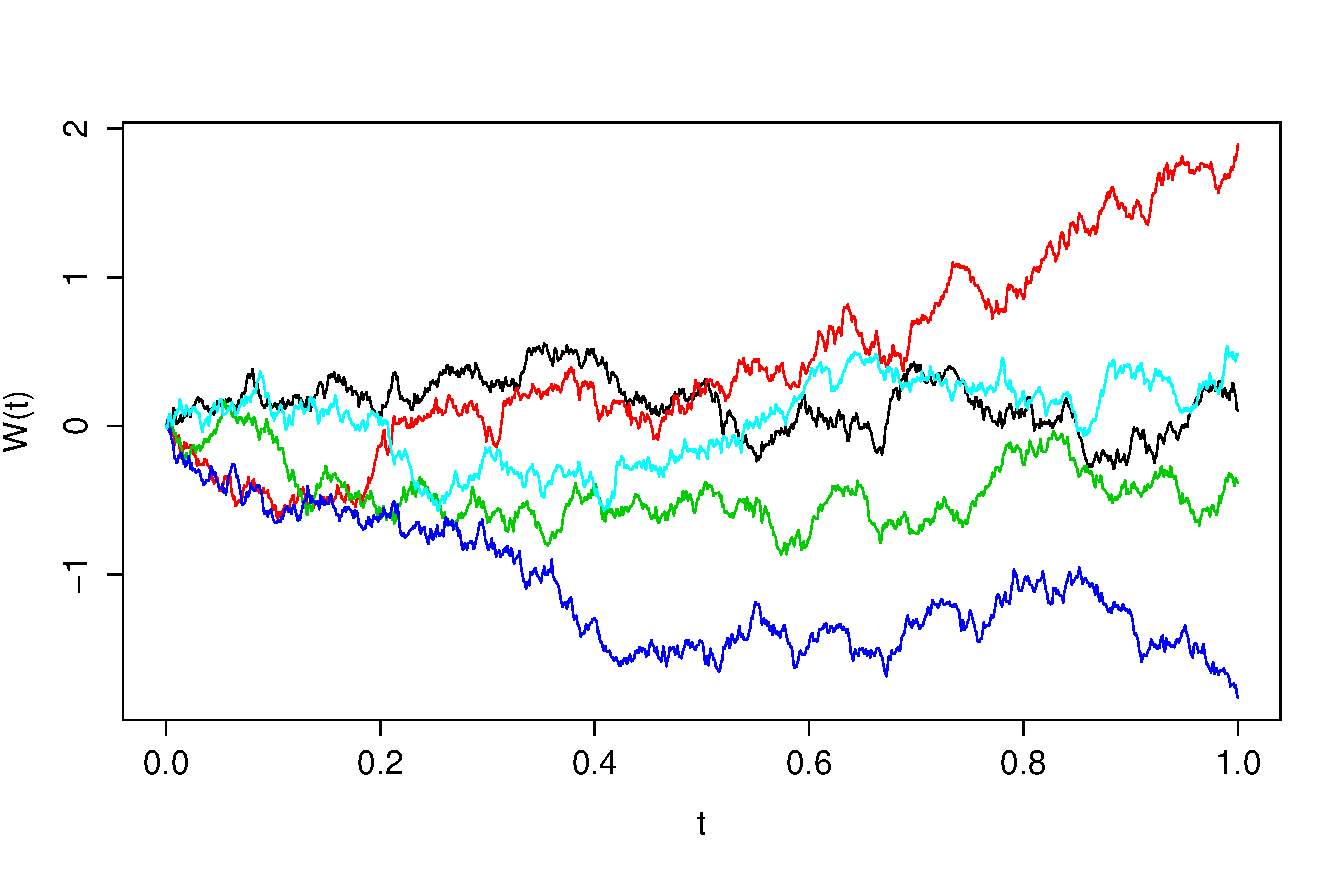
\includegraphics[width=13.5cm, clip, trim= 0 15 25 40]{IMG/WP_v2.pdf}
  \caption{Ukázka pěti trajektorií Wienerova procesu}  \label{WP_graf}
\end{figure}

Ceny aktiv na finačních trzích se podle teorie dokonalých trhů chovají zcela náhodně a nezávisle na předchozím vývoji.
Wienerův proces se tedy nabízí jako vhodný nástroj k popisu chování cen aktiv.
Při modelování ve finanční matematice využíváme procesy, které jsou zobecněním či modifikací Wienerova procesu. 
Uvažujme proces s nenulovým parametrem růstu, označovaným jako drift, a parametrem variability, jenž odpovídá směrodatné odchylce procesu.
\begin{definice}[Wienerův proces s driftem]\label{Wieneruv_proces_s_driftem}
Stochastický proces $X(t)$ definovaný jako
$$X(t)  = \mu\, t + \sigma\, W (t),$$
kde $\mu$ a $\sigma$ jsou konstanty a $W (t)$ je Wienerův proces,
se nazývá \textit{Wienerův proces  s driftem} $\mu$ a volatilitou $\sigma$.
\end{definice}
Pokud bychom chtěli využít tento proces k modelování cen podkladových aktiv, setkáme se s dvěma problémy.
Nejenže Wienerův proces s driftem může nabývat záporných hodnot, což je v rozporu s realitou chování cen podkladových aktiv, ale navíc by se model nechoval stejně při různých absolutních cenách aktiv. 
Aktivum s nižší současnou cenou by mělo větší riziko a také vyšší očekávaný výnos než aktivum s vyšší cenou.
Proto chceme proces upravit tak, aby absolutní očekávaný výnos a výše směrodatné odchylky byly proporcionální k ceně podkladového aktiva. 

Nejběžnější modifikací Wienerova procesu splňující tyto požadavky je Geometrický Wienerův proces, který v kontextu finanční matematiky použil poprvé Paul Samuelson \cite{samuelson1964rational}.
K rozšíření modelu používajícího tento proces přispěli především Fischer Black a Myron Scholes \cite{black1973pricing} a to zejména v kontextu oceňování opcí.

%V definici Geometrického Wienerova procesu využijeme stochastické diferenciální rovnice, které budou definovány v Kapitole \ref{SDR_kap}.
Geometrický Wienerův proces bývá často definován pomocí  stochastické diferenciální rovnice.
Proto uvádíme tento způsob definice, přestože budou definovány v Kapitole \ref{SDR_kap}.
\begin{definice}[Geometrický Wienerův proces]\label{Geometricky_Wieneruv_proces}
Stochastický proces $S(t)$, který je řešením stochastické diferenciální rovnice 
\begin{equation}\label{SDE_GWP}
\frac{\mathrm{d} S(t)}{S(t)} = \mu\,\mathrm{d}t + \sigma\,\mathrm{d}W (t), 
\end{equation}
kde  $\mu$ a $\sigma$ jsou konstanty a $W (t)$ je Wienerův proces,
se nazývá \textit{Geometrický Wienerův proces}.

Toto řešení můžeme vyjádřit následovně
\begin{equation}\label{GWP}
S(t) = S(0)\,\mathrm{e}^{X(t)},
\end{equation}
kde $X(t) = (\mu - \frac{\sigma^2}{2})\,t + \sigma W (t)$ je Wienerův proces s driftem (viz Definice \ref{Wieneruv_proces_s_driftem}).
\end{definice}
Člen $\mathrm{d}W(t)$ ve stochastické diferenciální rovnici \eqref{SDE_GWP} označuje infinitezimální přírůstek Wienerova procesu a $\mathrm{d}t$ je infinitezimální změna času.

Z Definice \ref{Geometricky_Wieneruv_proces} je zřejmé, že Geometrický Wienerův proces nabývá pouze kladných hodnot a jeho relativní přírůstky jsou nezávislé a mají stejné rozdělení. 
Kromě toho se s tímto procesem docela snadno pracuje ve výpočtech. 
Díky těmto vlastnostem se stal nejrozšířenějším modelem chování cen aktiv ve finanční matematice.

Ukázku trajektorií Geometrického Wienerova procesu s různými parametry driftu a volatility znázorňuje Obrázek \ref{GP_graf}.

\begin{figure}[!htbp]
  \centering 
	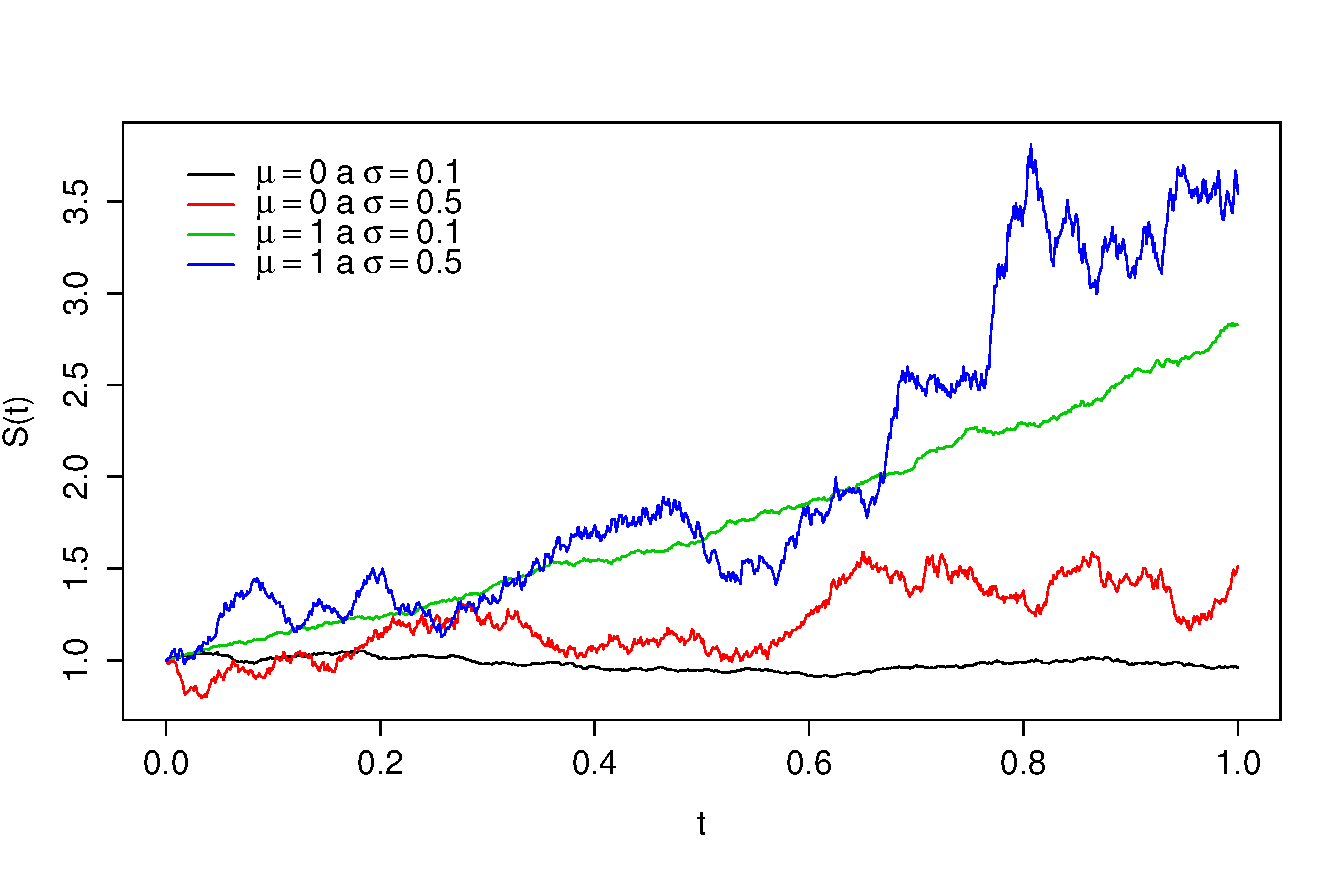
\includegraphics[width=13.5cm, clip, trim= 0 15 25 50]{IMG/GP_v2.pdf}
  \caption{Ukázka pěti trajektorií Geometrického Wienerova procesu s různými parametry driftu $\mu$ a volatility $\sigma$}  \label{GP_graf}
\end{figure}


\subsection{It\^oův proces}
Abychom mohli v následujícím textu zavést stochastický integrál definujme nejdříve širokou třídu procesů, tzv. It\^oových procesů.

%Zavedeme obecný stochasticky proces, který využijeme při konstrukci It\^oova lemmatu v další části. 
%Stochastický proces dostatečně obecný abychom mohli zavést stochastický integrál, pojmenovaný po známém matematikovi
Kiyosi It\^o byl japonský matematik, jenž modernizoval stochastické modely a jeho metody jsou dodnes používány v mnoha odvětvích vědy především ve financích a biologii.
Svou práci začal stavět v roce 1940 na základě dřívějších objevů Alberta Einsteina a Norberta Wienera.
V teorii stochastických procesů aplikoval metody diferenciálního a integrálního počtu.
%Matematický rámec pro popis chování stochastických procesů, který zkonstruoval se je po něm pojmenován It\^oův kalkul.
Matematický rámec zahrnující stochastické integrály a stochastické diferenciální rovnice vešel ve známost jako It\^oův kalkul.
Z významných It\^ových textů zmiňme 
článek \cite{ito1944} z roku 1944 obsahující konstrukci stochastického integrálu
a publikace \cite{ito1946} a
\cite{ito1951stochastic}, kde zavádí koncept stochastických diferenciálních rovnic.

Robert C. Merton, nositel Nobelovy za ekonomii, využívá teoretické poznatky Kiyosi It\^oa jako nástroj pro výzkum vývoje cen akcií v portfoliu a k oceňování finančních derivátů.
Tyto postupy více přiblížíme v Kapitole \ref{stoch_model} o stochastickém modelování.

\begin{definice}
Nechť $\{W(t):t\ge0\}$ je Wienerův proces na pravděpodobnostním prostoru $(\Omega,\mathcal{A},\mathsf{Pr})$.
Řekneme, že stochastický proces $\{f(t,\omega):t\ge~0\}$ je \textit{neanticipativní}, jestliže pro všechna $t\ge0$ hodnota $f(t,\omega)$ závisí jen na hodnotách Wienerova procesu do času $t$.
\end{definice}

\begin{definice}\label{M}
Nechť $W(t,\omega)$ je Wienerův proces na pravděpodobnostním prostoru $(\Omega,\mathcal{A},\mathsf{Pr})$.
Symbolem $M$ označme třídu stochastických procesů \linebreak$f(t,\omega):\langle0,\infty)\times\Omega\to\mathbb R$ takových, že
\begin{enumerate}
\item[1.] $f(t,\omega)$ je neanticipativní, 
\item[2.] $\text{E}\left[\int_0^Tf^2(t,\omega)\,\mathrm{d}t\right]<\infty.$ 
\end{enumerate}
\end{definice}

\begin{definice}[It\^oův proces]
Nechť $W(t,\omega)$ je Wienerův proces na pravděpodobnostním prostoru $(\Omega,\mathcal{A},\mathsf{Pr})$.
\textit{It\^oův proces} je stochastický proces
$$X(t,\omega)=X(0,\omega)+\int_0^tU(s,\omega)\,\mathrm{d}s+\int_0^tV(s,\omega)\,\mathrm{d}W(s,\omega),$$
kde $U(t,\omega)$ a $V(t,\omega)$ jsou stochastické procesy patřící do třídy $M$,
první integrál je Lebesgueův a druhý It\^oův (který je definován v Kapitole \ref{Ito_integral}).

Často se používá diferenciální tvar, nazývaný \textit{stochastický diferenciál},
$$\mathrm{d}X(t,\omega)=U(t,\omega)\,\mathrm{d}t+V(t,\omega)\,\mathrm{d}W(t,\omega).$$
\end{definice}

%Geometrický Wienerův proces je speciálním případem It\^oova procesu, kde $U(t,\omega)=\mu\,X(t,\omega)$ a $V(t,\omega))=\sigma X(t,\omega)$.

\subsection{Ornstein–Uhlenbeckův proces}\label{OU_kap}
Další často využívanou modifikací Wienerova procesu jsou stochastické procesy s tendencí vracet se k dlouhodobé rovnovážné hodnotě.
Nazývají se \textit{mean-reversion procesy} a nachází četné využití ve fyzice, matematice i ekonomii.
Ve finanční matematice se používají pro modelování úrokových sazeb, kurzů měn, cen komodit a volatility.
%Ornstein–Uhlenbeckův proces je další často využívanou modifikací Wienerova procesu.
%Mean-reversion jsou procesy, ve kterých se náhodná veličina vrací k dlouhodobé rovnovážné hodnotě. 
%Používají se zvláště pro modely úrokových sazeb. 
%V následujícím textu jsou uvedeny nejčastěji užívané procesy.

Holandští fyzikové Leonard Salomon Ornstein a George Eugene Uhlenbeck zformulovali jako první mean-reversion proces v roce 1930 a publikovali v textu \cite{OrnsteinUhlenbeck1930}. 

\begin{definice}[Ornstein–Uhlenbeckův proces]
\textit{Ornstein–Uhlenbeckův proces} je definován jako
\begin{equation}\label{OUP}
X_t = X_0\,\mathrm{e}^{-\theta t} + \mu\,(1-\mathrm{e}^{-\theta t}) + \mathrm{e}^{-\theta t}\int_0^t \sigma\,\mathrm{e}^{\theta s}\,\mathrm{d}W_s,
\end{equation}
kde parametr $\theta>0$ je koeficient rychlosti reverze, parametr $\mu\in\mathbb{R}$ je rovnovážná hodnota, parametr $\sigma>0$ je volatilita a $W_t$ je Wienerův proces.
Ornstein–Uhlenbeckův proces může být také definován jako řešení stochastické diferenciální rovnice
\begin{equation}\label{SDE_OUP}
\mathrm{d}X_t = \theta(\mu-X_t)\,\mathrm{d}t + \sigma\,\mathrm{d}W_t.
\end{equation}
\end{definice}

Ornstein–Uhlenbeckův proces je stacionární Gaussovský proces s ohraničeným rozptylem. 
Koeficient $\theta$ určuje rychlost přibližování k rovnovážné hodnotě $\mu$. %(nebo také střední hodnotě).
Čím je $\theta$ větší tím pohotověji proces reaguje na odchýlení od rovnováhy. 
Na rozdíl od Wienerova procesu nemá Ornstein–Uhlenbeckův proces konstantní koeficient driftu, jelikož závisí na jeho aktuální hodnotě.
Pokud je aktuální hodnota procesu $X_t$ menší než rovnovážná hodnota $\mu$, pak je koeficient driftu kladný.
Naopak když $X_t>\mu$, tak je koeficient driftu záporný.

Ukázku trajektorií Ornstein–Uhlenbeckova procesu s různými parametry najdeme na Obrázku \ref{OU_graf}.

\begin{figure}[!htbp]
  \centering 
	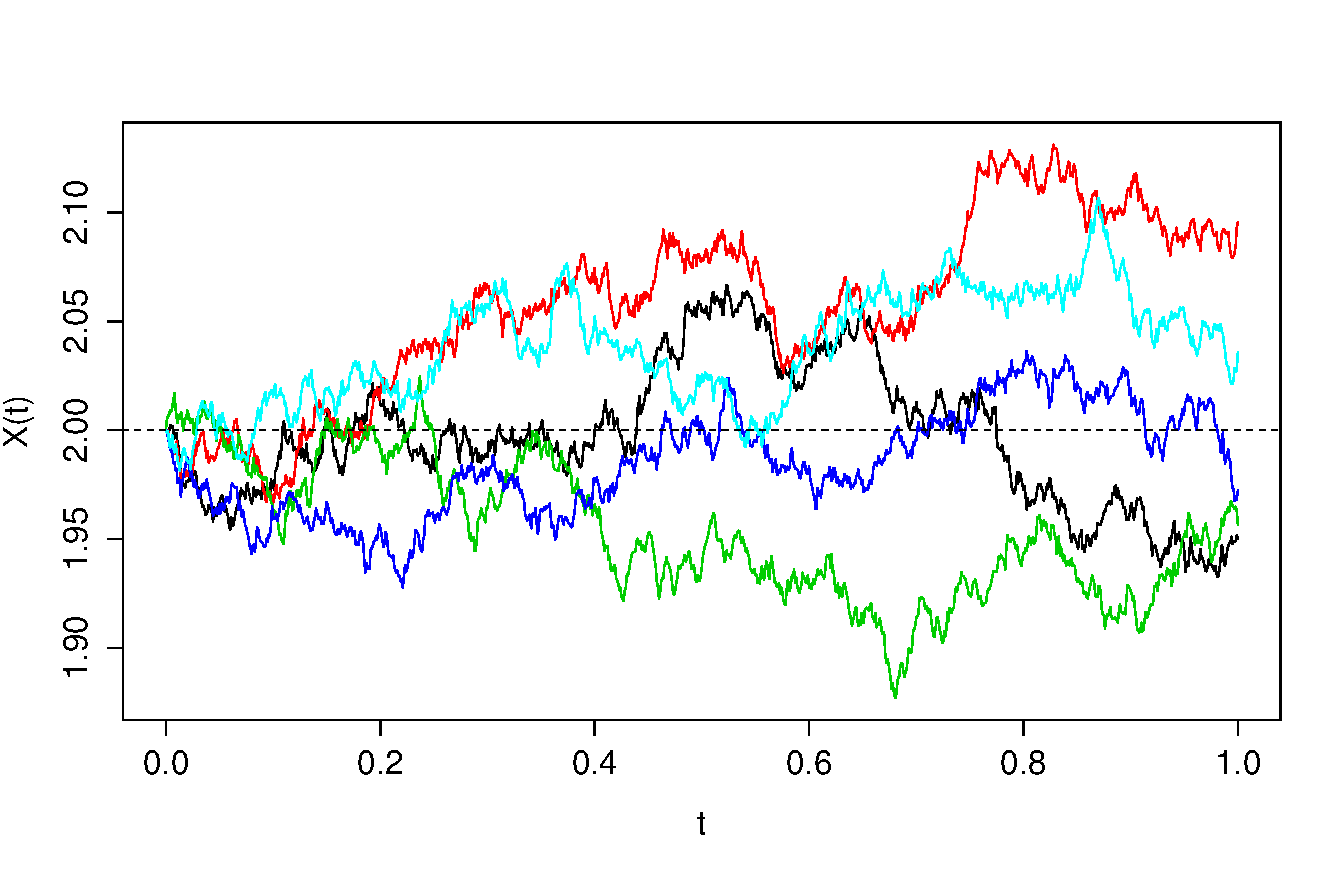
\includegraphics[width=13.5cm, clip, trim= 0 15 25 50]{IMG/OU_v4.pdf}
  \caption{Ukázka pěti trajektorií Ornstein–Uhlenbeckova procesu s parametry $\theta=1$, $\mu=2$ a  $\sigma=0,1$ a počáteční hodnotou $X_0=2$.}  \label{OU_graf}
\end{figure}

%\cite{Benth2016}
Vlastnostem Ornstein–Uhlenbeckova procesu (především stacionaritě) se zevrubně věnují Fred Espen Benth a Asma Khedher v knize \cite{podolskij2015fascination} z roku 2015, která je aktuální sbírkou prací vědců v oboru pravděpodobnosti, statistiky a jejich aplikací ve financích, ekonomii, fyzice, řízení rizika a systémů hromadné obsluhy.

\subsection{Mnohorozměrný Wienerův proces}
Chceme-li uvažovat finanční trh s více rizikovými aktivy a zabývat se jejich vzájemnými vztahy, musíme zavést vícerozměrný Wienerův proces.
Aplikaci tohoto vektorového stochastického procesu využijeme v dynamické teorii portfolia.

\begin{definice}
Standardní \textit{$n$-rozměrný Wienerův proces} je vektorový stochastický proces
$$\boldsymbol{W}(t) = (W_1(t), \dots, W_n(t))^\mathrm{T}$$
jehož složky $W_k(t)$ jsou nezávislé, standardní jednorozměrné Wienerovy procesy.
\end{definice}
%Wienerův proces je stavebním kamenem matematického modelování ve finanční matematice. 
%Tento stochastický proces se používá pro popis chování ceny aktiva v čase. 

Na Obrázku \ref{WP_2D_graf} vidíme ukázku trajektorie dvourozměrného Wienerova procesu.
\begin{figure}[!htbp]
  \centering 
	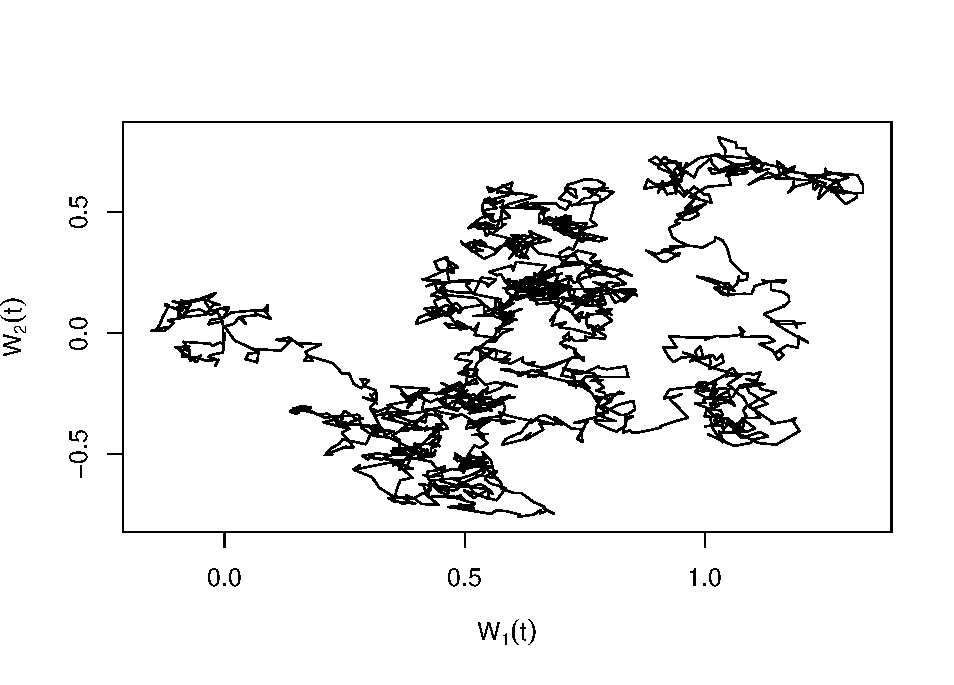
\includegraphics[width=13.5cm, clip, trim= 0 20 25 50]{IMG/WP_2D_v6.pdf}
  \caption{Ukázka trajektorie dvourozměrného Wienerova procesu}  \label{WP_2D_graf}
\end{figure}


%\section{It\^oův integrál a It\^oovo lemma}
\section{It\^oův integrální počet}\label{Ito_kalkul}
Chceme-li používat modely založené na stochastických procesech se spojitým časem neobejdeme se bez stochastického integrálního počtu.
Dále se proto budeme věnovat konstrukci stochastického integrálu, uvedeme It\^oovo lemma a vysvětlíme jeho přínos pro modelování ve finanční matematice.
Věty a lemmata budeme uvádět pouze bez důkazů, které jsou k nalezení v literatuře, viz například \cite{karatzas2012brownian}.

%Čerpat budeme z knih \cite{}...
Konstrukci stochastického integrálu podle Wienerova procesu představil v letech 1942--1944 Kiyosi It\^o v \cite{ito1942differential} a \cite{ito1944}. 
Obecnější stochastický integrál, který je založený na širší třídě stochastických procesů, zkonstruovali v roce 1967 Hiroshi Kunita a Shinzo Watanabe v \cite{kunita1967square}.

\subsection{It\^oův integrál}\label{Ito_integral}
Důležitým nástrojem pro řešení stochastických diferenciálních rovnic je It\^oův integrál (nazývaný též jen stochastický integrál).
Jeho zavedení je vyžadováno nediferencovatelností trajektorií Wienerova procesu.
Stochastický integrál budeme konstruovat obdobným způsobem jako Riemannův integrál.
Nejprve It\^oův integrál definujeme pro jednoduché procesy, následně definici rozšíříme na větší třídu procesů pomocí aproximace.

\begin{definice}\label{jednoduchafunkce}
Stochastický proces $S$ se nazývá \textit{jednoduchý}, %(nebo \textit{jednoduchá funkce}), 
jestliže existuje dělení $D=\{0=t_0<t_1<\cdots<t_{n-1}<t_n=T\}$ tak, že pro každé $t$, $t_k\le t<t_{k+1}$, $k=0,1,\dots,n-1$, je $S(t,\omega)=S_k(\omega)$, pro nějaké náhodné veličiny $S_k$. 
\end{definice}
Z Definice \ref{jednoduchafunkce} vyplývá, že trajektorie jednoduchého procesu je po částech konstantní. 

\begin{definice}
Nechť $S$ je jednoduchý proces a zaveďme označení \linebreak$\Delta W_k=W(t_{k+1},\omega)-W(t_k,\omega)$.
Pak
$$\int_0^TS\,\mathrm{d}W=\sum_{k=0}^{n-1}S_k\Delta W_k$$
se nazývá \textit{It\^oův integrál} procesu $S$ na intervalu $\langle 0,T\rangle$.
\end{definice}

Pomocí limitního přechodu rozšíříme definici It\^oova integrálu pro jednoduché procesy na integrál pro obecný stochastický proces.

\begin{lemma} \label{itoint}
Nechť $f$ je stochastický proces patřící do třídy $M$ dle Definice \ref{M}.
Pak existuje posloupnost jednoduchých procesů $\{f_n:n\in\mathbb N\}$ tak, že pro $n\to\infty$ platí
$$\mathrm{E}\left[\int_0^T\big[f(t)-f_n(t)\big]^2\mathrm{d}t\right]\longrightarrow0.$$
\end{lemma}

\begin{definice}\label{Ito_int}
Nechť $\{f_n:n\in\mathbb N\}$ je posloupnost jednoduchých procesů z lemmatu \ref{itoint}.
Pro obecný proces $f(t,\omega)\in M$ definujeme \textit{It\^oův integrál} předpisem
$$\int_0^Tf(t,\omega)\,\mathrm{d}W=\lim_{n\to\infty}\int_0^Tf_n(t,\omega)\,\mathrm{d}W.$$
\end{definice}
Definice \ref{Ito_int} není závislá na volbě aproximující posloupnosti $f_n$ viz \cite{oksendal2003stochastic}.

\subsection{It\^oovo lemma}
It\^oovo lemma je nástrojem pro práci s It\^oovým integrálem a stochastickými diferenciálními rovnicemi.
Říká, že It\^oovy procesy tvoří uzavřenou třídu vzhledem ke skládání s hladkými funkcemi.
Kiyosi It\^o jej publikoval v roce 1944 v článku \cite{ito1944}.
\begin{veta}[It\^oovo lemma]
Nechť $X(t,\omega)$ je It\^oův proces se stochastickým diferenciálem
$$\mathrm{d}X=U\,\mathrm{d}t+V\,\mathrm{d}W.$$
Nechť $g(t,x):(0,\infty)\times\mathbb R\to\mathbb R$ je dvakrát spojitě diferencovatelná funkce.
Potom $Y(t)=g(t,X(t))$ je také It\^oův proces.
Jeho stochastický diferenciál má tvar
\begin{alignat*}{2}
\mathrm{d}Y=\frac{\partial g}{\partial t}\mathrm{d}t+\frac{\partial g}{\partial x}\,\mathrm{d}X+\frac12\frac{\partial^2 g}{\partial x^2}(\mathrm{d}X)^2=\left[\frac{\partial g}{\partial t}+\frac{\partial g}{\partial x}U+\frac12\frac{\partial^2 g}{\partial x^2}V^2\right]\mathrm{d}t+\frac{\partial g}{\partial x}V\mathrm{d}W.
\end{alignat*}
\end{veta}

It\^oovo lemma můžeme považovat za analogii Taylorova rozvoje v integrálním počtu.
Tento důležitý vztah stochastické analýzy budeme využívat pro oceňování finančních derivátů, jejichž hodnota je závislá na hodnotě podkladového aktiva.


%%%%%%%%%%%%%%%%%%{Stochastické diferenciální rovnice}

\section{Stochastické diferenciální rovnice}
%http://artax.karlin.mff.cuni.cz/~masas7am/bakalarka/bakalarka.pdf
%Stochastické diferenciální rovnice (SDR) se používají při modelování dynamických jevů, v nichž hraje roli náhoda. 
%Za první počiny v této oblasti lze považovat pokusy o matematický model Brownova pohybu z přelomu 19. a 20. století. 
%Ale až stochastický integrál, který definoval v roce 1944 japonský matematik Kiyoshi It\^o, a s ním spojený It\^oův kalkul umožnil formulovat a řešit skutečné stochastické diferenciální rovnice. 
%Ty od té doby našly uplatnění v mnoha oborech -- od fyziky přes biologii až po modelování cen akcií ve finanční matematice.
%vývoj a chování v čase
%Pomocí diferenciálních rovnic lze popsat celou řadu zákonitostí, které se objevují v přírodních a společenských vědách.
%Řešeními diferenciálních rovnic jsou funkce, které popisují vlastnosti zkoumaných jevů. 

Pomocí diferenciálních rovnic jsme schopni popsat množství zákonitostí platných ve vědeckých oborech přírodních, společenských i ekonomických.
Řešení diferenciálních rovnic jsou funkce popisující vlastnosti zkoumaných jevů.
Stochastické diferenciální rovnice (SDR) nám umožňují modelovat dynamiku \textit{náhodných jevů}.
K formulování a řešení SDR je využíván It\^oův kalkul popsaný v Kapitole \ref{Ito_kalkul}.
Aplikací stochastických diferenciálních rovnic ve stochastickém modelování se zabýváme v Kapitole \ref{stoch_model}, kde uvádíme modely popisující vývoj a chování cen finančních aktiv v čase.

Základní studijní literaturou nám byla monografie Bernta {\O}ksendala \cite{oksendal2003stochastic}.
Pracovali jsme také s texty \cite{cyganowski1998maple} a \cite{cyganowski2002elementary}, které napsal Sasha Cyganowski s kolektivem autorů.

%Stochastická diferenciální rovnice je rovnice popisující přírůstky stochastického procesu v čase. 
%Ve finanční matematice se používá například pro popis přírůstku hodnoty nějakého aktiva.
\subsection{Úvod do teorie stochastických diferenciálních rovnic}\label{SDR_kap}
Na úvod do teorie SDR uveďme základní definice, používané značení a podmínky řešitelnosti.
\begin{definice}[Stochastická diferenciální rovnice]
Nechť $\alpha(t,x)$ a $\beta(t,x)$ jsou funkce dvou proměnných $\alpha,\beta:\mathcal{T}\times\mathbb{R}\to\mathbb{R}$.

\textit{Stochastickou diferenciální rovnicí (SDR)} rozumíme rovnici
\begin{equation}\label{SDR_reseni}
X(t)=X_0+\int_{t_0}^t\alpha(s,X(s))\,\mathrm{d}s+\int_{t_0}^t\beta(s,X(s))\,\mathrm{d}W(s),
\end{equation}
kde první integrál je Lebesgueův a druhý integrál je It\^oův definovaný v Kapitole \ref{Ito_integral}.
Častěji se s SDR setkáváme v jejím diferenciálním tvaru
\begin{align}\label{SDR_def}
\mathrm{d}X(t)&=\alpha(t,X(t))\,\mathrm{d}t+\beta(t,X(t))\,\mathrm{d}W(t),\\%\qquad 
X(t_0)&=X_0.\notag
\end{align}
Náhodnou veličinu $X(t_0)=X_0$ nazýváme \textit{počáteční podmínkou SDR} a stochastický proces $X(t)$ splňující vztah \eqref{SDR_reseni}, nazýváme \textit{řešením SDR} na $\mathcal{T}$.
\end{definice}
%Uvažujme o existenci a jednoznačnosti řešení SDR.

Uvažujme $n$ stochastických procesů $X_1(t),\dots,X_n(t)$, které popisují nějakým způsobem související náhodné jevy, například vývoj cen $n$ různých akcií na kapitálovém trhu. 
K popisu chování takových procesů v čase slouží soustavy stochastických diferenciálních rovnic (někdy označované jako systémy SDR) .
\begin{definice}[Soustava $n$ stochastických diferenciálních rovnic]
Nechť
%$$\boldsymbol\alpha(\boldsymbol t,\boldsymbol X(t))=\big(\alpha^1(t,\boldsymbol{X}(t)),\dots,\alpha^n(t,\boldsymbol{X}(t))\big)^\mathrm{T}$$
$$\boldsymbol\alpha( t,\boldsymbol x)=\big(\alpha^1( t,\boldsymbol{x}),\dots,\alpha^n(t,\boldsymbol{x})\big)^\mathrm{T}$$
je spojitá vektorová funkce $\boldsymbol\alpha:\mathcal{T}\times\mathbb{R}^n\to\mathbb{R}^n$.
Pro $j=1,\dots,m$ označíme 
%$$\boldsymbol\beta^{j}(\boldsymbol t,\boldsymbol X(t))=\big(\beta^{1,j}(t,\boldsymbol{X}(t)),\dots,\beta^{n,j}(t,\boldsymbol{X}(t))\big)^\mathrm{T}$$
$$\boldsymbol\beta^{j}(t,\boldsymbol x)=\big(\beta^{1,j}(t,\boldsymbol{x}),\dots,\beta^{n,j}(t,\boldsymbol{x})\big)^\mathrm{T}$$
a nechť $\boldsymbol{B}=(\boldsymbol\beta^{1},\dots,\boldsymbol\beta^{m})$ je spojitá maticová funkce $\boldsymbol{B}:\mathcal{T}\times\mathbb{R}^n\to\mathbb{R}^{n\times m}$.

Pro $j=1,\dots,m$ rozumíme \textit{soustavou stochastických diferenciálních rovnic} systém
\begin{equation}\label{SSDR_reseni}
X^i(t)=X^i_0+\int_{t_0}^t\alpha^i(s,\boldsymbol{X}(s))\,\mathrm{d}s+\sum_{j=1}^m\int_{t_0}^t\beta^{i,j}(s,\boldsymbol{X}(s))\,\mathrm{d}W^j(s),\\%\qquad 
\end{equation}
kde první integrál je opět Lebesgueův a integrály v sumě jsou It\^oovy stochastické integrály.
Diferenciální tvar soustav SDR zapíšeme ve formě
\begin{align}\label{SSDR_def}
\mathrm{d}X^i(t)&=\alpha^i(t,\boldsymbol{X}(t))\,\mathrm{d}t+\sum_{j=1}^m\beta^{i,j}(t,\boldsymbol{X}(t))\,\mathrm{d}W^j(t),\\%\qquad 
X^i(t_0)&=X^i_0.\notag
\end{align}
kde $\boldsymbol{W}({t})=(W^1(t),\dots,W^m(t))^\mathrm{T}$ je $m$-rozměrný Wienerův proces.
\end{definice}

\subsubsection{Existence a jednoznačnost řešení}
Teorie o existenci a jednoznačnosti řešení stochastických diferenciálních rovnic a jejich soustav vychází z podobných přístupů jako v případě obyčejných diferenciálních rovnice.
Zejména se předpokládají určité vlastnosti koeficientů rovnic jako je lokální Lipschitzova spojitost.
Následující věta shrnuje podmínky existence a jednoznačnosti řešení soustavy stochastických diferenciálních rovnic.
\begin{veta}[O existenci a jednoznačnosti řešení soustav SDR]
Nechť jsou $\boldsymbol\alpha:\mathcal{T}\times\mathbb{R}^n\to\mathbb{R}^n$ a $\boldsymbol{B}:\mathcal{T}\times\mathbb{R}^n\to\mathbb{R}^{n\times m}$ měřitelné funkce splňující podmínku
\begin{equation}\label{glob_Lipschitzova_podminka}
||\boldsymbol\alpha( t,\boldsymbol x)||+||\boldsymbol{B}( t,\boldsymbol x)||\leq C(1+{||\boldsymbol x||}),
\end{equation}
pro každé $\boldsymbol x\in\mathbb{R}^n$ a $t\in \mathcal{T}$ a pro nějakou kladnou konstantu $C$.
Dále nechť funkce $\boldsymbol\alpha$ a $\boldsymbol B$ splňují podmínku
\begin{equation}\label{loc_Lipschitzova_podminka}
||\boldsymbol\alpha( t,\boldsymbol x)-\boldsymbol\alpha( t,\boldsymbol y)||+||\boldsymbol{B}( t,\boldsymbol x)-\boldsymbol{B}( t,\boldsymbol y)||\leq D||\boldsymbol x-\boldsymbol y||,
\end{equation}
pro každé $\boldsymbol x , \boldsymbol y\in\mathbb{R}^n$ a $t\in \mathcal{T}$ a pro nějakou kladnou konstantu $D$.
Dále nechť $\boldsymbol X_0$ je náhodný vektor, který může být závislý na hodnotách Wienerova procesu $\boldsymbol W(t)$ pouze v čase $t_0$,%nezávislý na trajektorii Wienerova procesu $\boldsymbol W(t)$ 
a platí
\begin{equation}\label{podminka_tri}
\mathrm{E}\left[||\boldsymbol X_0||^2\right]<\infty.
\end{equation} 
Pak má soustava stochastických diferenciálních rovnic \ref{SSDR_def} jednoznačné řešení na $\mathcal{T}$.
\end{veta}
\begin{proof}
Viz \cite{oksendal2003stochastic}.
\end{proof}

\subsection{Numerické metody řešení stochastických diferenciálních rovnic}
%citace: Peter E. Kloeden Eckhard Platen Henri Schurz Numerical Solution of SDE Through Computer Experiments
%An Introduction to Stochastic Processes with Applications to Biology Linda J. S. Allen
Numerické metody využíváme v případě kdy není možno určit řešení SDR analyticky.
Základním principem numerických metod je diskretizace proměnných.
Numerická metoda určí aproximaci řešení v diskrétních časových hodnotách a spojitou aproximaci řešení získáme použitím interpolačních metod.

Pro obeznámení s numerickými metodami řešení SDR a jejich soustav jsme zvolili monografii Petera Erise Kloedena, Eckharda Platena a Henriho Schurze \cite{kloeden1997}.
Dalším zdrojem nám byla již zmiňovaná kniha \cite{cyganowski2002elementary} autorů Cyganowski, Kloeden a Ombach.
Využití numerických řešení SDR při oceňování finančních derivátů popisuje Timothy Sauer \cite{sauer2012numerical}.

\subsubsection{Eulerova metoda}
Základní numerická metoda pro řešení obyčejných diferenciálních rovnic je pojmenovaná po významném švýcarském matematikovi a fyzikovi Leonhardu Paulu Eulerovi, který ji zpracoval ve své knize \textit{Institutionum calculi integralis} publikované roku 1768, \cite{euler1768institutionum}.
Tato metoda byla v roce 1955 modifikována japonským matematikem Gisiro Maruyamou \cite{maruyama1955continuous}, aby umožňovala řešit SDR.
Jedná se o nejjednodušší metodu, která slouží ke konstrukci složitějších numerických metod pro řešení SDR.

Uvažujme It\^oův proces $X(t)$, který je řešením SDR definované vztahem \eqref{SDR_def}.
Nechť $\{t_n\}_{n=0}^N\subseteq \mathcal{T}$ je časová posloupnost, kde pro všechna $n$ platí $t_n<t_{n+1}$.
Tato  posloupnost se nazývá \textit{diskretizace} časové proměnné.
V Eulerově metodě diferenciál $\mathrm{d}X(t)$ aproximujeme přírůstkem stochastického procesu $\Delta X_n=X(t_{n+1})-X(t_n)$.
Hodnota $X(t_{n+1})$ je aproximována pomocí hodnoty $X(t_{n})$ v předcházejícím časovém kroku.
\begin{definice}\label{Euler_def}
Nechť $X_n$ značí aproximaci řešení $X(t_{n})$ stochastické diferenciální rovnice \eqref{SDR_def} v čase $t_n$.
Pak \textit{Eulerova metoda} řešení SDR je definována rekurzívním vztahem
\begin{equation}\label{Euler}
X_{n+1}=X_n+\alpha(t_n,X_n)\Delta_n+\beta(t_n,X_n)\Delta W_n,
\end{equation}
kde $\Delta_n=\int_{t_n}^{t_{n+1}}\mathrm{d}t=t_{n+1}-t_n$ je délka časového intervalu $(t_n,t_{n+1})$
a $\Delta W_n=\int_{t_n}^{t_{n+1}}\mathrm{d}W(t)=W(t_{n+1})-W(t_n)$ je přírůstek Wienerova procesu $W$ v čase $(t_n,t_{n+1})$.

Zobecníme-li Eulerovu metodu pro soustavu $m$ stochastických diferenciálních rovnic \eqref{SSDR_def}, pak vztah pro $i$-tou složku aproximace řešení je definován předpisem
\begin{equation}\label{Euler_soustava}
X_{n+1}^i=X_n^i+\alpha^i(t_n,\boldsymbol{X}_n)\Delta_n+\sum_{j=1}^m\beta^{i,j}(t_n,\boldsymbol{X}_n)\Delta W_n^j.
\end{equation}
%kde $\boldsymbol{X}$ je $m$-rozměrný Wienerův proces.
\end{definice}

\textit{Eulerova aproximace} je spojitý stochastický proces, který v daných časech $\{t_n\}_{n=0}^N\subseteq \mathcal{T}$ splňuje vztah \eqref{Euler} a hodnoty mezi těmito časovými body získáme pomocí lineární interpolace.

Většinou se předpokládá, že časová posloupnost $\{t_n\}_{n=0}^N\subseteq \mathcal{T}$ je ekvidistantní. 
Důležitou problematikou při používání numerických metod je způsob výpočtu $\Delta W_n$.
Z vlastnosti Wienerova procesu plyne, že $\Delta W_n\sim\mathsf{N}(0, \Delta_n)$.

\subsubsection{Milsteinova metoda}
Milsteinova numerická metoda řešení SDR je popsána v knihách Eckharda Platena \cite{platen2010numerical} a Paula Glassermana \cite{glasserman2003monte}.
Tuto metodu poprvé představil Grigori N. Milstein ve svém článku \cite{milstein1974approximate} v roce 1974.
Metoda se snaží zdokonalit aproximaci difuzního členu tím, že aditivně připojuje třetí člen k Eulerovově diskretizaci.
%Přitom se využívá stochastický Taylorův rozvoj. 
Pro odvození podoby tohoto členu je využíváno  It\^oovo lemma, které je aplikováno na koeficienty stochastického procesu.
Následnými úpravami a zanedbáním členů vyšších řádů získáme vztah uvedený v definici \ref{Milstein_def}.
Poznamenejme, že pro správné fungování Milsteinovy metody je narozdíl od Eulerovy metody potřebný předpoklad diferencovatelnosti funkce $\beta(t,\boldsymbol{x})$ podle složek $\boldsymbol{x}$.
\begin{definice}\label{Milstein_def}
Nechť $X_n$ značí aproximaci řešení $X(t_{n})$ stochastické diferenciální rovnice \eqref{SDR_def} v čase $t_n$.
Pak \textit{Milsteinova metoda} řešení SDR je definována rekurzívním vztahem
\begin{align}\label{Milstein}
X_{n+1}&=X_n+\alpha(t_n,X_n)\Delta_n+\beta(t_n,X_n)\Delta W_n \\ \notag
&+\frac12\beta(t_n,X_n)\beta'(t_n,X_n)\big((\Delta W_n)^2-\Delta_n\big),
\end{align}
kde $\beta'(t_n,X_n)$ je derivace $\beta(t_n,X_n)$ podle $X_n$,
$\Delta_n=\int_{t_n}^{t_{n+1}}\mathrm{d}t=t_{n+1}-t_n$ je délka časového intervalu $(t_n,t_{n+1})$
a $\Delta W_n=\int_{t_n}^{t_{n+1}}\mathrm{d}W(t)=W(t_{n+1})-W(t_n)$ je přírůstek Wienerova procesu $W$ v čase $(t_n,t_{n+1})$.

Poznamenejme, že v případě, kdy koeficient $\beta(t,X(t))=\beta(t)$ nezávisí na procesu $X(t)$, pak $\beta'(t,X(t))=0$ a Milsteinova metoda je identická s metodou Eulerovou.

Zobecníme-li Milsteinovu metodu pro soustavu $m$ stochastických diferenciálních rovnic \eqref{SSDR_def}, pak vztah pro $i$-tou složku aproximace řešení je definován předpisem
\begin{align}\label{Milstein_soustava}
X_{n+1}^i&=X_n^i+\alpha^i(t_n,\boldsymbol{X}_n)\Delta_n+\sum_{j=1}^m\beta^{i,j}(t_n,\boldsymbol{X}_n)\Delta W_n^j \\ \notag 
%&+\sum_{j=1}^m\sum_{k=1}^m\beta^{i,j}(t_n,\boldsymbol{X}_n)\sum_{l=1}^m\frac{\partial\beta^{i,k}(t_n,\boldsymbol{X}_n)}{\partial X_l}\int_{t_n}^{t_{n+1}}\!\int_{t_n}^{t}\mathrm{d}W^k(s)\mathrm{d}W^j(t).
&+\sum_{j=1}^m\sum_{k=1}^m\beta^{i,j}(t_n,\boldsymbol{X}_n)\sum_{l=1}^m\frac{\partial\beta^{i,k}(t_n,\boldsymbol{X}_n)}{\partial X_l}\int_{t_n}^{t_{n+1}}\big(W^k(t)-W^k(t_n)\big)\,\mathrm{d}W^j(t).
\end{align}
%kde $\boldsymbol{X}$ je $m$-rozměrný Wienerův proces.
\end{definice}

Pro $j=k$ je možno It\^oův integrál $\int_{t_n}^{t_{n+1}}\big(W^k(t)-W^k(t_n)\big)\,\mathrm{d}W^j(t)$ vyjádřit pomocí časového přírůstku $\Delta_n$ a přírůstku Wienerova procesu $\Delta W^k_n$ jako 
$$\int_{t_n}^{t_{n+1}}\big(W^k(t)-W^k(t_n)\big)\,\mathrm{d}W^k(t)=\frac12\big((\Delta W^k_n)^2-\Delta_n\big).$$
Avšak pro $j\neq k$ obdobné vyjádření neexistuje a integrál je nutné simulovat.
V uvedené literatuře lze nalézt různé přístupy k tomuto problému.
Například simulace využívající distribuční funkce, nebo substituování jednodušší náhodnou veličinou, případně zavedení zjednodušujících předpokladů o funkci volatility $\beta(t,\boldsymbol{x})$.
%Nicméně tyto úvahy jsou již nad rámec této práce.

\subsubsection{Konvergence}
Chceme-li posuzovat kvalitu jednotlivých numerických metod řešení SDR a~vzájemně je porovnávat, zkoumáme odchylku aproximace řešení od přesného řešení (tzv. chybu aproximace).
V literatuře se běžně setkáváme se dvěma kategoriemi kriterií sloužící k posouzení konvergence aproximace k~přesnému řešení.
Jsou to silná konvergenční kritéria a slabá konvergenční kritéria. 
Uvědomme si, že v každém čase $t_n$ jsou jak přesné řešení SDR $X(t_{n})$, tak jeho aproximace $X_n$ náhodné veličiny.
Slabá konvergence sleduje velikost odchylky středních hodnot řešení SDR a jeho aproximace, naproti tomu silná konvergence uvažuje střední hodnotu odchylek $X(t_{n})$ a $X_n$.
%Uvažujme za jakých podmínek aproximace řešení SDR konverguje k přesnému řešení pro zmenšující se časový krok.  
%Uvědomme si, že jak přesné řešení SDR $X(t_{n})$, tak jeho aproximace $X_n$ jsou v každém čase $t_n$ náhodné veličiny.
%Budeme definovat dva typy konvergence.
%Slabá konvergence sleduje velikost odchylky středních hodnot řešení SDR a jeho aproximace, naproti tomu silná konvergence uvažuje střední hodnotu odchylek $X(t_{n})$ a $X_n$.
%K porovnání jednotlivých numerických metod řešení SDR slouží mimo jiné řád konvergence.

\begin{definice}\label{konvergence_weak_def}
Uvažujme diskretizaci času $\{t_n\}_{n=0}^N\subseteq \mathcal{T}$.%\subseteq\langle 0,T\rangle$.
Označme $X(t_n)$ přesné řešení SDR v čase $t_n$ a $X_n$ příslušnou aproximaci řešení v čase $t_n$.
Řekneme, že aproximace \textit{slabě konverguje} k řešení v čase $t_n$, jestliže platí
\begin{equation}
\lim_{\Delta_n\to0}\left|\mathsf{E}\big(f(X(t_n))\big)-\mathsf{E}\big(f(X_n)\big)\right|=0
\end{equation}
pro každou polynomiální funkci $f(x)$.

Řekneme, že numerická metoda má \textit{slabý řád konvergence $q$}, jestliže existuje kladná konstanta $K$ taková, že pro všechna $n$ platí
\begin{equation}\label{konvergence_weak_vztah}
\left|\mathsf{E}\big(f(X(t_n))\big)-\mathsf{E}\big(f(X_n)\big)\right|\leq K\Delta^q,
\end{equation}
kde  $\Delta=\max_{0\leq n\leq N-1}\Delta_n$.
Levá strana vztahu \eqref{konvergence_weak_vztah} se nazývá slabá chyba aproximace.
\end{definice}
Pro různou volbou polynomu $f(x)$ dostáváme konvergenci různých momentů řešení SDR.

\begin{definice}\label{konvergence_def}
Uvažujme diskretizaci času $D=\{t_n\}_{n=0}^N\subseteq \mathcal{T}$.
Řekneme, že aproximace \textit{silně konverguje} k řešení v čase $T\in\mathcal{T}$, jestliže platí
\begin{equation}
\lim_{\Delta\to0}\left[\sup_{D:||D||=\Delta}\mathsf{E}\big(|X(T)-X_D(T)|\big)\right]=0
\end{equation}
kde $||D||=\max_{0\leq n\leq N-1}\Delta_n$, $X(T)$ je přesné řešení SDR v čase $T$ a $X_D(T)$ značí aproximaci řešení v čase $T$ příslušnou diskretizaci $D$.

Řekneme, že numerická metoda má \textit{silný řád konvergence $p$}, jestliže existuje kladná konstanta $K$ taková, že pro všechna $D$ platí
\begin{equation}\label{konvergence_vztah}
\mathsf{E}\big(|X(T)-X_D(T)|\big)\leq K\Delta^p,
\end{equation}
kde  $\Delta=\max_{0\leq n\leq N-1}\Delta_n$.
Levá strana vztahu \eqref{konvergence_vztah} se nazývá silná chyba aproximace.
\end{definice}
Poznamenejme, že silná konvergence implikuje slabou konvergenci.

Abychom získali co nejpřesnější aproximaci trajektorií řešení stochastické diferenciální rovnice, používáme metody s co největším silným řádem konvergence.
Ačkoli je známo, že Eulerova numerická metoda řešení obyčejných diferenciálních rovnic má silný řád konvergence 1, 
tak stochastická Eulerova numerická metoda má řád konvergence $\frac12$.
Tuto skutečnost dokázali roku 1972 Gikhman a Skorokhod v \cite{gikhman1972stochastic}.
Naproti tomu Milsteinova numerická metoda má silný řád konvergence jedna.
Platí tedy, že v obecném případě, kdy se v koeficientu volatility $\beta(t,x)$ vyskytuje proměnná $x$, Milsteinova metoda konverguje k přesnému řešení SDR rychleji než Eulerova metoda (spolu se zmenšováním časového kroku $\Delta$).

%\end{comment}
%%%%%%%%%%%%%%%%%%{Stochastické modelování}

\chapter{Stochastické modelování}\label{stoch_model}

Stochastický model slouží k popisu dějů, ve kterých je přítomná náhodná složka.
%náhodných jevů, které vyjadřujeme pomocí stochastických procesů.
Pomocí stochastického modelu lze simulovat průběh děje a pozorovat jeho chování při nastavení různých parametrů modelu.
Aplikace stochastického modelování a simulace chování dějů umožňují nejen jejich popis, ale také jejich analýzu.
Na základě analýzy chování modelu a simulací můžeme získat informace pro řízení procesů a k rozhodování.
%Metody stochastického modelování mají význam pro podporu rozhodovacího procesu v situacích za neurčitosti a pro řízení procesů a dějů náhodnou složkou.

V této práci se zaměříme na ekonomické modely popisující, jak se na finančním trhu díky nabídce a poptávce formují ceny finančních aktiv.
%ekonomické modely nabídky a poptávky
Finanční aktiva poskytují investorovi nárok na budoucí příjem.
Mezi finanční aktiva patří především podkladová aktiva, finanční deriváty a peníze.

Modelovat budeme vývoj ceny jak podkladových aktiv, tak finančních derivátů.
Podkladové aktivum je nástroj, jehož v čase se měnící cena slouží jako základ pro pohyb ceny finančních derivátů.
Podkladovými aktivy mohou být akcie, úrokové míry, komodity, měny, akciové indexy a mnoho dalších finančních instrumentů.
%Obecně jakékoliv aktivum, jehož cena se vyvíjí v čase.
Chování cen aktiv vykazuje stochastický charakter a cenové změny jsou náhodné a nepředvídatelné.
%, k jehož modelování využíváme stochastické diferenciální rovnice.
%K modelování stochastického charakteru chování cen podkladových aktiv využíváme stochastické diferenciální rovnice.
Kolísání cen aktiv v čase je způsobené vzájemným působením nabídky a poptávky na trhu.
%Teorie efektivního trhu tvrdí, že ceny aktiv velmi rychle plně odrážejí veškeré tržní informace.
Mezi základní teoretická východiska v teorii finančních trhů patří hypotéza efektivního trhu,
která tvrdí, že ceny aktiv velmi rychle plně odrážejí veškeré tržní informace
a zcela reflektují všechna očekávání investorů ohledně budoucího vývoje cen aktiv.

%Pro přehled uvadíme základní teorie finančních trhů:
%\begin{itemize}
%\item[-]Ceny aktiv jsou výsledkem mnoha náhodných událostí a nelze je předpovídat.
%cenové zmeny jsou náhodné a nepredvídatelné
%\\\item[-]Teorie efektivního trhu tvrdí, že ceny aktiv velmi rychle plně odrážejí veškeré tržní informace.
%V každém případě dlouhodobě je vývoj akciových kurzů odrazem trendů ve
%\\\item[-]Kolísání cen aktiv v čase je způsobené vzájemným působením nabídky a poptávky na trhu.
%Úroková míra je určována trhem -- bankami, které přijímají vklady a poskytují úvěry, a subjekty působícími na kapitálovém trhu.
%Cenová změna aktiv je výsledkem mnoha náhodných událostí a nelze ji předpovídat.
%cenotvorba
%\end{itemize}

Teorie finančních trhů je podrobně zpracována v české literatuře.
Z velkého množství textů odkažme na \cite{rejnus2011}, \cite{fuchsfinancni} a \cite{veselainvestovani} se kterými jsme při psaní práce pracovali.
Stochastickým modelováním v ekonomii se pak zabývá převážně zahraniční literatura, ze které jsme nejvíce využívali \cite{hull}, \cite{wilmott1995mathematics} a \cite{karatzas1998methods}.

\section{Stochastické modelování cen finančních aktiv}
%na základě střetu nabídky a poptávky možné určit rovnovážnou cenu 

%Tržní hodnota akcie, kterou určuje burza je tedy především oceněním hospodaření podniku.
%Hodnota akcie je tedy dána jejím hospodařením. Zájem o akcii pak tvoří její cenu, protože převis poptávky ji zvyšuje a převis nabídky snižuje. Kdo chce znát cenu akcie, zjistí si ji na burze. Cena akcie je prostě dána její podnikatelskou hodnotou, jak ji vidí akcionáři a obchodníci na burzách.
%Finanční teorie zpravidla definuje investiční instrumenty (investiční nástroje) jako aktiva, která investorovi (majiteli) přináší nějaký nárok na budoucí příjem (např. dividendy, kuponové platby, úroky či kapitálové výnosy).

%Aplikace SDR ve financích najdeme v \cite{karatzas2012brownian}. Už citováno.

%Citace:  \cite{baxter1996financial} a  \cite{franke2004statistics}

V následující části popíšeme konstrukci matematických modelů používaných ve finanční matematice pro popis vývoje cen aktiv na finančních trzích.
V Kapitole \ref{WP_kap} jsme uvažovali nad požadavky kladenými na chování stochastického procesu, který můžeme využít k modelování cen aktiv, aby byl model smysluplný.
Zrekapitulujme kvalitativní znaky modelu aktiv:
\begin{itemize}
\item[-] v dlouhodobém časovém horizontu mají ceny aktiv přibližně exponenciální růst,
\item[-] fluktuace cen aktiv je náhodná,
\item[-] ceny aktiv jsou nezáporné,
\item[-] model je univerzální pro různé úrovně cen aktiv.
\end{itemize}
%Modeling with Itô Stochastic Differential Equations Od autorů: Edward Allen (googlebooks) - multidimenzní Ito formule 
%Dynamic Asset Pricing Theory Od autorů: Darrell Duffie (googlebooks) - Black-Scholes
Jak už bylo naznačeno v Kapitole \ref{WP_kap}, základní model splňující uvedené požadavky je založen na Geometrickém Wienerově procesu. 
Model byl zaveden a prosazen Paulem Samuelsonem \cite{samuelson1965proof}.
Budeme tedy předpokládat, že proces popisující vývoj ceny aktiva v čase se řídí následující stochastickou diferenciální rovnicí %následujícím modelem
\begin{equation}\label{risk_asset_model}
\mathrm{d}P(t)=P(t)\,\mu(t)\,\mathrm{d}t+P(t)\,\sigma(t)\,\mathrm{d}W(t),
\end{equation}
kde $P(t)$ je cena aktiva v čase $t$, $\mu(t)$ a $\sigma(t)$ jsou stochastické procesy a $W(t)$  je jednorozměrný Wienerův proces.
Tento model předpokládá, že na trhu je pouze jedno rizikové aktivum.

Model pro vývoj ceny aktiv na trhu, který předpokládá existenci $n$ rizikových aktiv je dán jako
\begin{equation}\label{multi_risk_asset_model}
\mathrm{d}P_j(t)=P_j(t)\,\mu_j(t)\,\mathrm{d}t+P_j(t)\sum_{k=1}^{n}\xi_{jk}(t)\,\mathrm{d}W_k(t),
\end{equation}
kde $P_j(t)$ je cena aktiva $j$ v čase $t$, $\mu_j(t)$ a $\xi_{jk}(t)$ jsou stochastické procesy a $\boldsymbol{W}(t)=(W_1(t),\dots,W_n(t))^\mathrm{T}$ je $n$-rozměrný Wienerův proces. 
%Pro více informací o mnohorozměrných modelech viz \cite{etheridge2002course}.

Chování ceny bezrizikového aktiva je popsáno modelem
\begin{equation}\label{risk-free_asset_model}
\mathrm{d}B(t)=B(t)\,r_f(t)\,\mathrm{d}t,
\end{equation}
kde $B(t)$ je cena bezrizikového aktiva v čase $t$ a $r_f(t)$ je bezriziková úroková míra.

\begin{figure}[!htbp]
  \centering 
	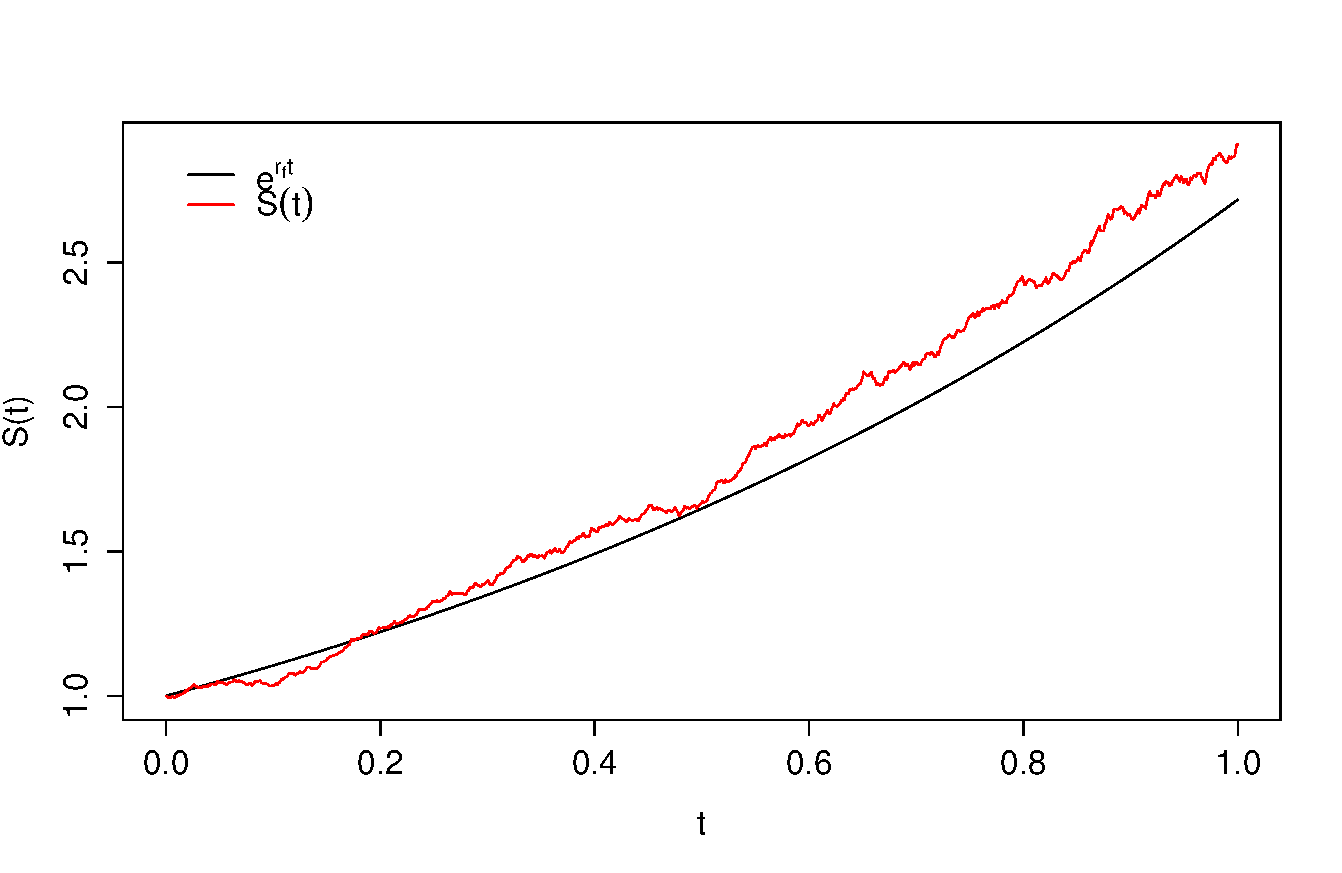
\includegraphics[width=13.5cm, clip, trim= 0 15 25 50]{IMG/GWP_RFA_v4.pdf}
  \caption{Model ceny bezrizikového aktiva s úrokovou mírou $r_f=1$ a~model ceny rizikového aktiva s parametry $\mu=1$ a  $\sigma=0,1$ a počáteční hodnotou $S(0)=1$.}  \label{asset_model_graf}
\end{figure}

\subsection{Black–Scholesův model}
Odvození Black–Scholesova modelu je srozumitelně zpracováno v učebnici Alison Etheridge \cite{etheridge2002course}.
 \cite{baxter1996financial}.

Samofinancující strategie spočívá ve vytvoření takového portfolia, které má stejné základní charakteristiky jako finanční derivát. 
Toto portfolio nazýváme \textit{replikační portfolio}.
Stává se z jednoho rizikového a jednoho bezrizikového aktiva.

\begin{definice}
\textit{Portfolio} $\big(\phi(t),\psi(t)\big)$ je dvojice stochastických procesů $\phi(t)$ a $\psi(t)$, která udává podíl rizikových a bezrizikových aktiv držených v čase $t$.
Stochastický proces $\phi(t)$ je neanticipativní (podíl rizikových aktiv v portfoliu v čase $t$ může být ovlivněn pouze informacemi známými do času $t$).
\end{definice}
Procesy $\phi(t)$ a $\psi(t)$ nabývají kladných hodnot, nicméně pokud je na trhu povolen tzv. \textit{prodej na krátko (short sell)} mohou nabývat i hodnot záporných.
Prodej na krátko je spekulativní metoda obchodování na finančním trhu, kdy investor očekává pokles ceny finančního aktiva.
Investor si finanční aktivum vypůjčí od věřitele na předem stanovenou dobu a ihned ho prodá třetí straně.
Nejpozději za stanovenou dobu investor nakoupí finanční aktivum na trhu a vrátí jej věřiteli.
Rozdíl mezi prodejní a nákupní cennou je výsledný zisk nebo ztráta.
Kvůli vysoké rizikovosti je prodej na krátko často regulován a v některých zemích dokonce zcela zakázán, neboť investor může dosáhnout pouze omezeného zisku, ale teoreticky neomezené ztráty.

\section{Stochastické modelování úrokových sazeb}
Na rozdíl od akcií nebo komodit vykazuje chování úrokových sazeb následující příznačné vlastnosti. %zvláštnosti.
Úrokové sazby se pohybují v určitém rozmezí a %obvykle nerostou do nekonečna ani neklesají pod nulu.
mají tendenci se vracet k určité rovnovážné hodnotě.
Tento jev se nazývá \textit{mean reversion} -- reverze k průměrné hodnotě.
Stochastické modely, které popisují chování úrokových sazeb musí tedy brát v úvahu výše uvedené vlastnosti.

%Vašíček 1977 model úrokové sazby

Jednofaktorové modely krátkodobých úrokových měr předpokládají, že okamžitá úroková míra $r$ je charakterizovaná pomocí řešení stochastické diferenciální rovnice, která má tvar
%dvoufaktorove r odvozuji od dvou informaci x, y
\begin{equation}\label{model_urok_miry}
\mathrm{d}r(t)=\mu(t,r)\,\mathrm{d}t+\sigma(t,r)\,\mathrm{d}W(t)
\end{equation}
Deterministická část procesu je $\mu(t, r)\,\mathrm{d}t$ a určuje drift ve vývoji úrokové míry, tj. trend, kterým by se úroková míra řídila za předpokladu neexistence náhodných vlivů, volatilita $\sigma(t, r)\,\mathrm{d}w$ určuje vlastnosti náhodných výchylek.

\subsection{Vašíčkův model}
Vašíčkův model je jednofaktorový model, který předpokládá, že okamžitá úroková míra $r$ je charakterizovaná pomocí řešení stochastické diferenciální rovnice, která má tvar
\begin{equation}\label{Vasickuv_model}
\mathrm{d}r(t) = \kappa(\theta - r(t))\,\mathrm{d}t + \sigma\,\mathrm{d}W(t)
\end{equation}
kde $\kappa$, $\theta$ a $\sigma$ jsou konstanty. 
Jejichž význam je následující:
\begin{itemize}
\item[-] $\theta$ je limitní úroková míra, 
\item[-] $\kappa$ je rychlost reverze k limitní úrokové míře, 
\item[-] $\sigma$ je volatilita.
\end{itemize}

Drift této rovnice je $\mu(t, r) = \kappa ( \theta - r(t))$, volatilita této rovnice je $\sigma(t, r) = \sigma$. 
Uvedený model má vlastnost mean reversion, což znamená, že drift táhne proces krátkodobých úrokových měr k průměrné hodnotě dané konstantou $\theta$. 
Daný proces je Ornstein-Uhlenbeckův proces definovaný v Kapitole \ref{OU_kap}.

Mezi výhody Vašíčkova modelu patří, že existuje explicitní vyjádření odhadů parametrů $\theta$, $\kappa$ a  $\sigma$ metodou maximální věrohodnosti.
Mezi nevýhody Vašíčkova modelu patří, že připouští i záporné úrokové míry, k tomu dojde v případě, kdy se úroková míra přiblízí nule a volatilita je stále táž konstanta.
Tuto chybu odstraňuje Cox - Ingersoll - Rossův model (CIR model), který je ve tvaru 
\begin{equation}\label{CIR_model}
\mathrm{d}r(t) = \mu(t, r)\,\mathrm{d}t + \sigma\sqrt{r(t, r)}\,\mathrm{d}W(t)
\end{equation}
Je vidět, že při malých úrokových mírách je malá také volatilita a převažuje vliv driftu. Kdyby byla úroková míra dokonce nulová, bude volatilita také nulová a změna úrokové míry je dána pouze driftem, který bude v tomto případě kladný.
Úroková míra v čase $t + \Delta t$ je rovna $r(t) + \kappa ( \theta - r(t))\Delta t + \sigma \Delta W$.

\subsection{Hull-Whitův model}
\begin{equation}\label{H-W_model}
 \mathrm{d}r(t)=[\theta(t)-\alpha r] \mathrm{d}t+\sigma \mathrm{d}W(t),
\end{equation}
kde
%\begin{description}
%\item [$ \mathrm{d}r$] The change in the interest rate after a small change in time, $ \mathrm{d}t$.
%\item [$\alpha$   ] Mean reversion rate.
%\item [$\sigma$   ] Volatility of the interest rate.
%\item [$ \mathrm{d}W$] A Wiener process.
%\item [$\theta(t)$] Drift function defined as
%\end{description}
\begin{equation}
\theta(t)=F'_{t}(0,t)+\alpha F(0,t)+\frac{\sigma^2}{2 \alpha}(1- \mathrm{e}^{-2\alpha t}),
\end{equation}
\begin{description}
\item[$F(0,t)$] Instantaneous forward rate at time $t$.
\item[$F'_{t}(0,t)$] Partial derivative of $F$ with respect to time $t$.
\end{description}
%%%%%%%%%%%%%%%%%%{Teorie portfolia}

\chapter{Teorie portfolia}
\textit{Portfolio} je soubor finančních aktiv držených fyzickou nebo právnickou osobou zvanou \textit{investor}.

%%%%%%%%%%%%%%%%%%{Základní charakteristiky portfolia}

\section{Základní charakteristiky portfolia}
V teorii portfolia se investoři snaží minimalizovat investiční riziko a~zároveň maximalizovat investiční výnos. 
Avšak se zvyšováním očekávaného výnosu je spojen i~růst rizika, proto základním problémem při optimalizaci portfolia je hledání kompromisu mezi maximalizací výnosu a~minimalizací rizika spojeného s~investováním.  
V následující části popíšeme a~definujeme tyto základní charakteristiky portfolia.

\subsection{Výnosnost}
\textit{Míra výnosnosti} (nebo \textit{relativní výnosnost}) aktiva je charakteristika, která udává zisk nebo ztrátu z~investice za pevně stanovené období vyjádřená v~poměru k~množství investovaných prostředků.

\begin{definice}
Investujeme-li $Y$ korun do nějakého aktiva $j$ v čase $t$, pak korunová hodnota investice v čase $t+\Delta t$ bude $[1+r_j(t,t+\Delta t)]Y$, kde  $r_j(t,t+\Delta t)$ definujeme jako \textit{míru výnosnosti}.  
\end{definice}
 
Relativní výnosnost bývá často označována pouze jako \textit{výnosnost}.
Vzhledem k~tomu, že výnosnost aktiva je pro investora nejistá (s výjimkou bezrizikového aktiva), budeme ji v~teorii portfolia chápat jako náhodnou veličinu. % a~budeme ji značit $r_j$.
Rozdělení pravděpodobnosti této náhodné veličiny nelze určit, nicméně v~teorii portfolia se obejdeme bez znalosti rozdělení a~využijeme pouze dále uvedené základní charakteristiky náhodné veličiny.

První z~těchto charakteristik bude střední hodnota výnosnosti aktiva, kterou označíme $\mathsf{E}(r_j)=\mu_j$.
V~teorii portfolia se ve spojitosti s~touto charakteristikou setkáváme s~pojmem \textit{očekávaná výnosnost}.
Rozptyl výnosnosti aktiva označíme $\mathsf{D}(r_j)=\sigma_j^2$.

Následující značení využijeme při definicích charakteristik porfolia.
Nechť $\boldsymbol{r}=(r_1,\dots,r_n)^\mathrm{T}$ značí náhodný vektor, jehož složky jsou výnosnosti aktiv držených v~portfoliu $p$.
Relativní podíly aktiv, ze kterých se skládá portfolio, se nazývají \textit{váhy} portfolia.
Vektor vah portfolia budeme značit $\boldsymbol{X}=(X_1,\dots,X_n)^\mathrm{T}$ a~přirozeně platí, že $\sum_{j=1}^nX_j=1$. 
Mezi základní charakteristiky portfolia patří jeho \textit{výnosnost}, která je dána jako $r_p=\boldsymbol{X}^\mathrm{T}\boldsymbol{r}=\sum_{j=1}^nX_jr_j$ a~je rovněž náhodnou veličinou.   
Jedním z faktorů pro výběr portfolia v Markowitzově teorii je \textit{očekávaná výnosnost portfolia}, kterou označíme $\mathsf{E}(r_p)=\mu_p$ a je zřejmé, že platí $\mu_p=\sum_{j=1}^nX_j\mu_j$.

\subsection{Riziko}
\textit{Riziko} popisuje míru nejistoty, že se skutečná výnosnost investice bude lišit od očekávané výnosnosti.  
\textit{Riziko aktiva} definujeme jako směrodatnou odchylku výnosnosti aktiva a~označíme ho $\sqrt{\mathsf{D}(r_j)}=\sigma_j$.
Analogicky je \textit{riziko portfolia} definováno jako směrodatná odchylka výnosnosti portfolia a~značeno $\sqrt{\mathsf{D}(r_p)}=\sigma_p$.  

Riziko celého portfolia v~sobě zahrnuje nejen rizika jednotlivých aktiv v~portfoliu, ale také riziko z~vzájemné závislosti výnosností jednotlivých aktiv.
Míra vzájemné závislosti dvou výnosností je mimo jiné popsána jejich kovariancí. 
Kovarianci výnosnosti aktiva~$j$ a~výnosnosti aktiva~$k$ označíme $\mathsf{C}(r_j,r_k)=\sigma_{jk}$.
Snadno se dá dokázat, že $\sigma_p=\sqrt{\sum_{j=1}^n\sum_{k=1}^nX_jX_k\sigma_{jk}}$.
Riziko portfolia je dalším faktorem pro výběr portfolia v~Markowitzově teorii.  


%%%%%%%%%%%%%%%%%%%%%%%%{Klasická teorie portfolia}


\section{Klasická teorie portfolia}\label{KTP}

Základy klasické teorie portfolia položil Harry Markowitz svým článkem v roce 1952 \cite{markowitz}, ve kterém upozornil na nutnost zohledňovat při výběru portfolia nejenom očekávanou výnosnost, ale i riziko změny výnosnosti.
Jeho největším přínosem bylo kvantifikování očekávaného výnosu a rizika portfolia. 
Dalším přínosem byl matematický důkaz výhod diverzifikace, které byly do té doby chápány pouze intuitivně.
Markowitz zkonstruoval množinu všech dostupných portfolií v prostoru výnos -- riziko, zavedl pojem \textit{efektivní množina portfolií}, ze které investor vybírá optimální portfolio pomocí indiferenčních křivek popisujících investorův vztah k riziku.
Konstrukcí množiny dostupných (nebo přípustných) portfolií se bude věnovat Kapitola \ref{Markowitz_kap}. 
Na Obrázku \ref{obr_Markowitz} je znázorněna množina přípustných portfolií  a množina efektivních portfolií v prostoru výnosnost -- riziko. 

\begin{figure}[!htbp] 
  \centering 
  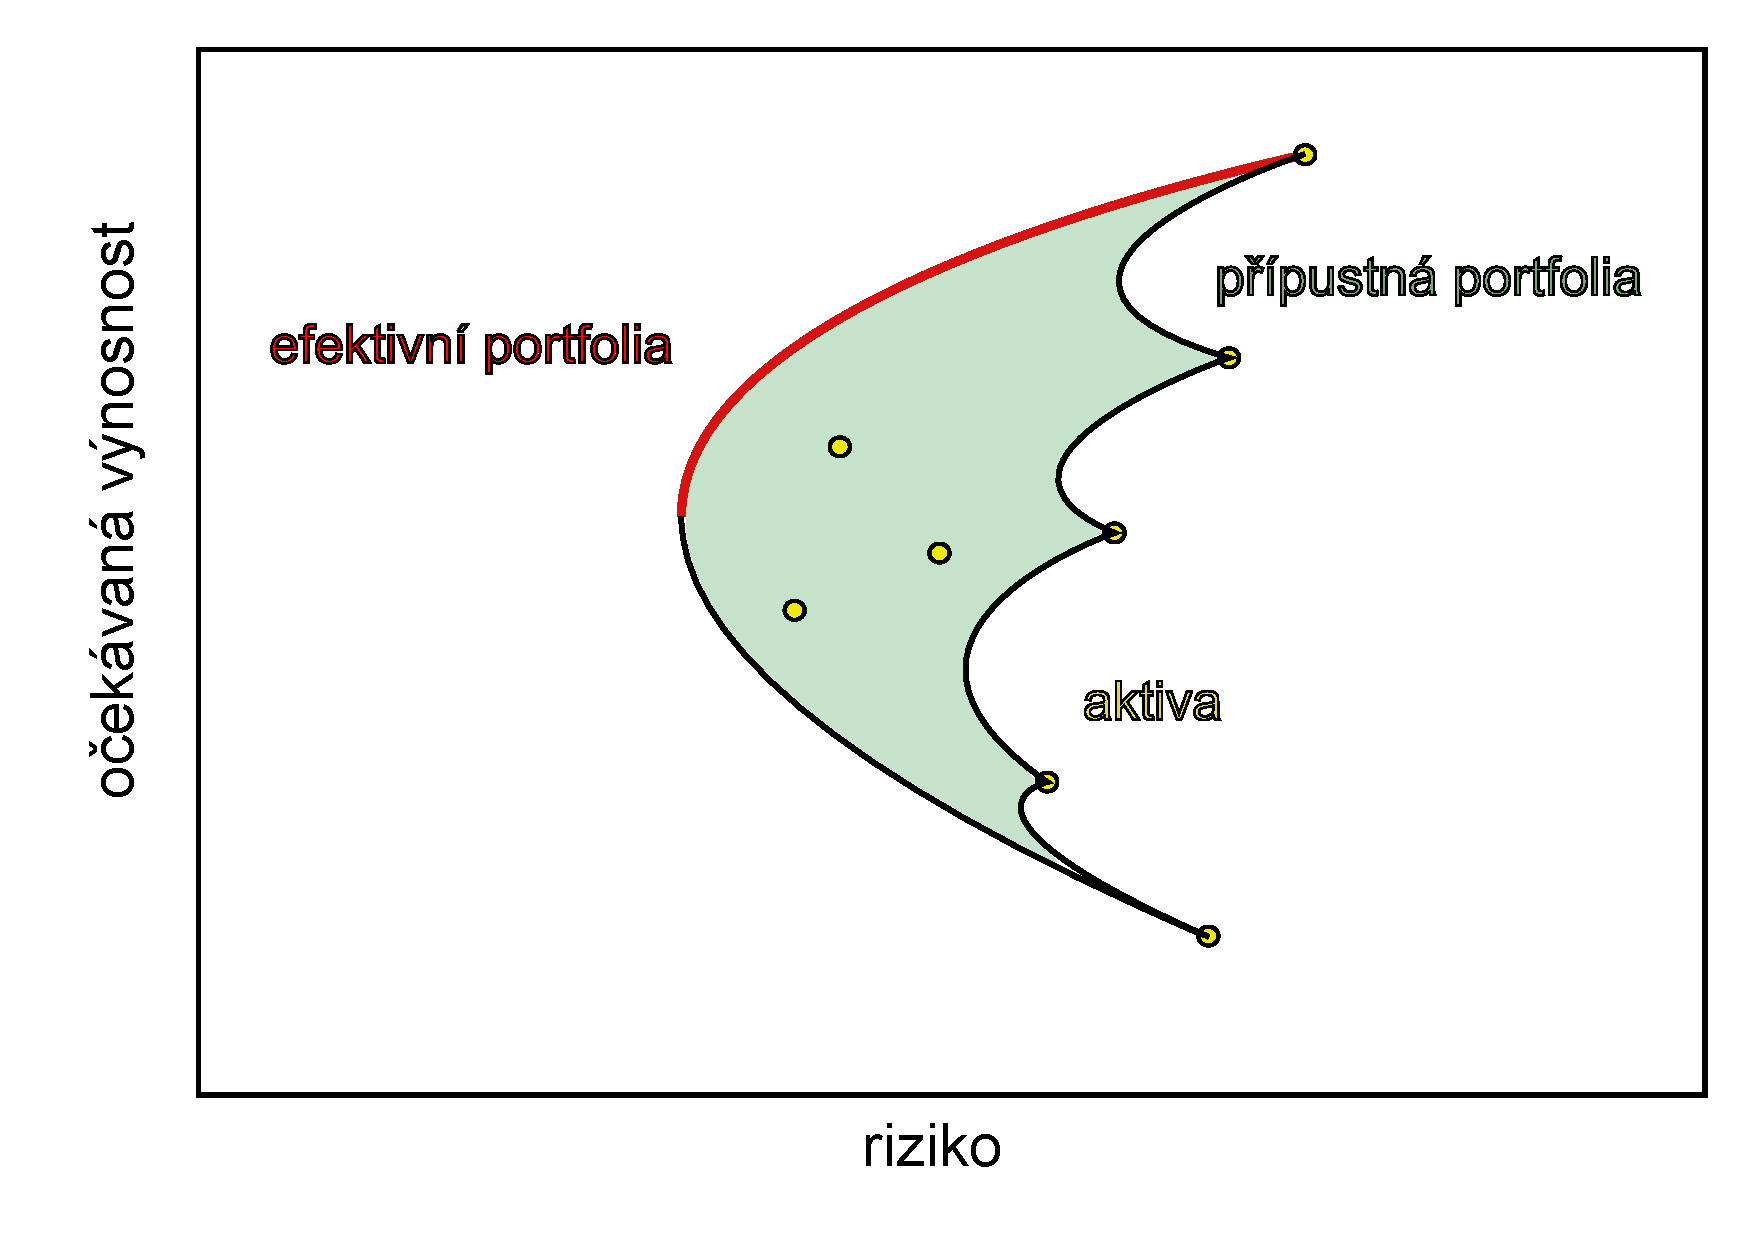
\includegraphics[width=11cm]{IMG/graf_2a.pdf}
  \caption{Množina přípustných portfolií  a množina efektivních portfolií v prostoru výnosnost -- riziko dle Markowitzovy teorie portfolia.} 
  \label{obr_Markowitz}
\end{figure}

V roce 1958 rozšířil James Tobin \cite{tobin} Markowitzův model o možnost investování do bezrizikového aktiva.
\textit{Bezrizikové aktivum} má jistý výnos a tedy nulové riziko.
To má velký vliv především na efektivní množinu portfolií, která je tvořena tečnou k původní Markowitzově efektivní množině procházející bezrizikovým aktivem, což je zobrazeno na Obrázku \ref{obr_Tobin_1}.
V bodě dotyku pak leží tzv. tangenciální portfolio (viz Obrázek \ref{obr_Tobin_2}).
Postup investora při hledání optimálního portfolia shrnuje Tobinův separační teorém, který se později vžil v souvislosti s CAPM, který bude popsán v další části. % \ref{kapitola_CAPM}.
Investor prvně určí tangenciální portfolio a následně ho zkombinuje s bezrizikový aktivem podle svých rizikových preferencí.

\begin{figure}[!htbp]
  \centering 
  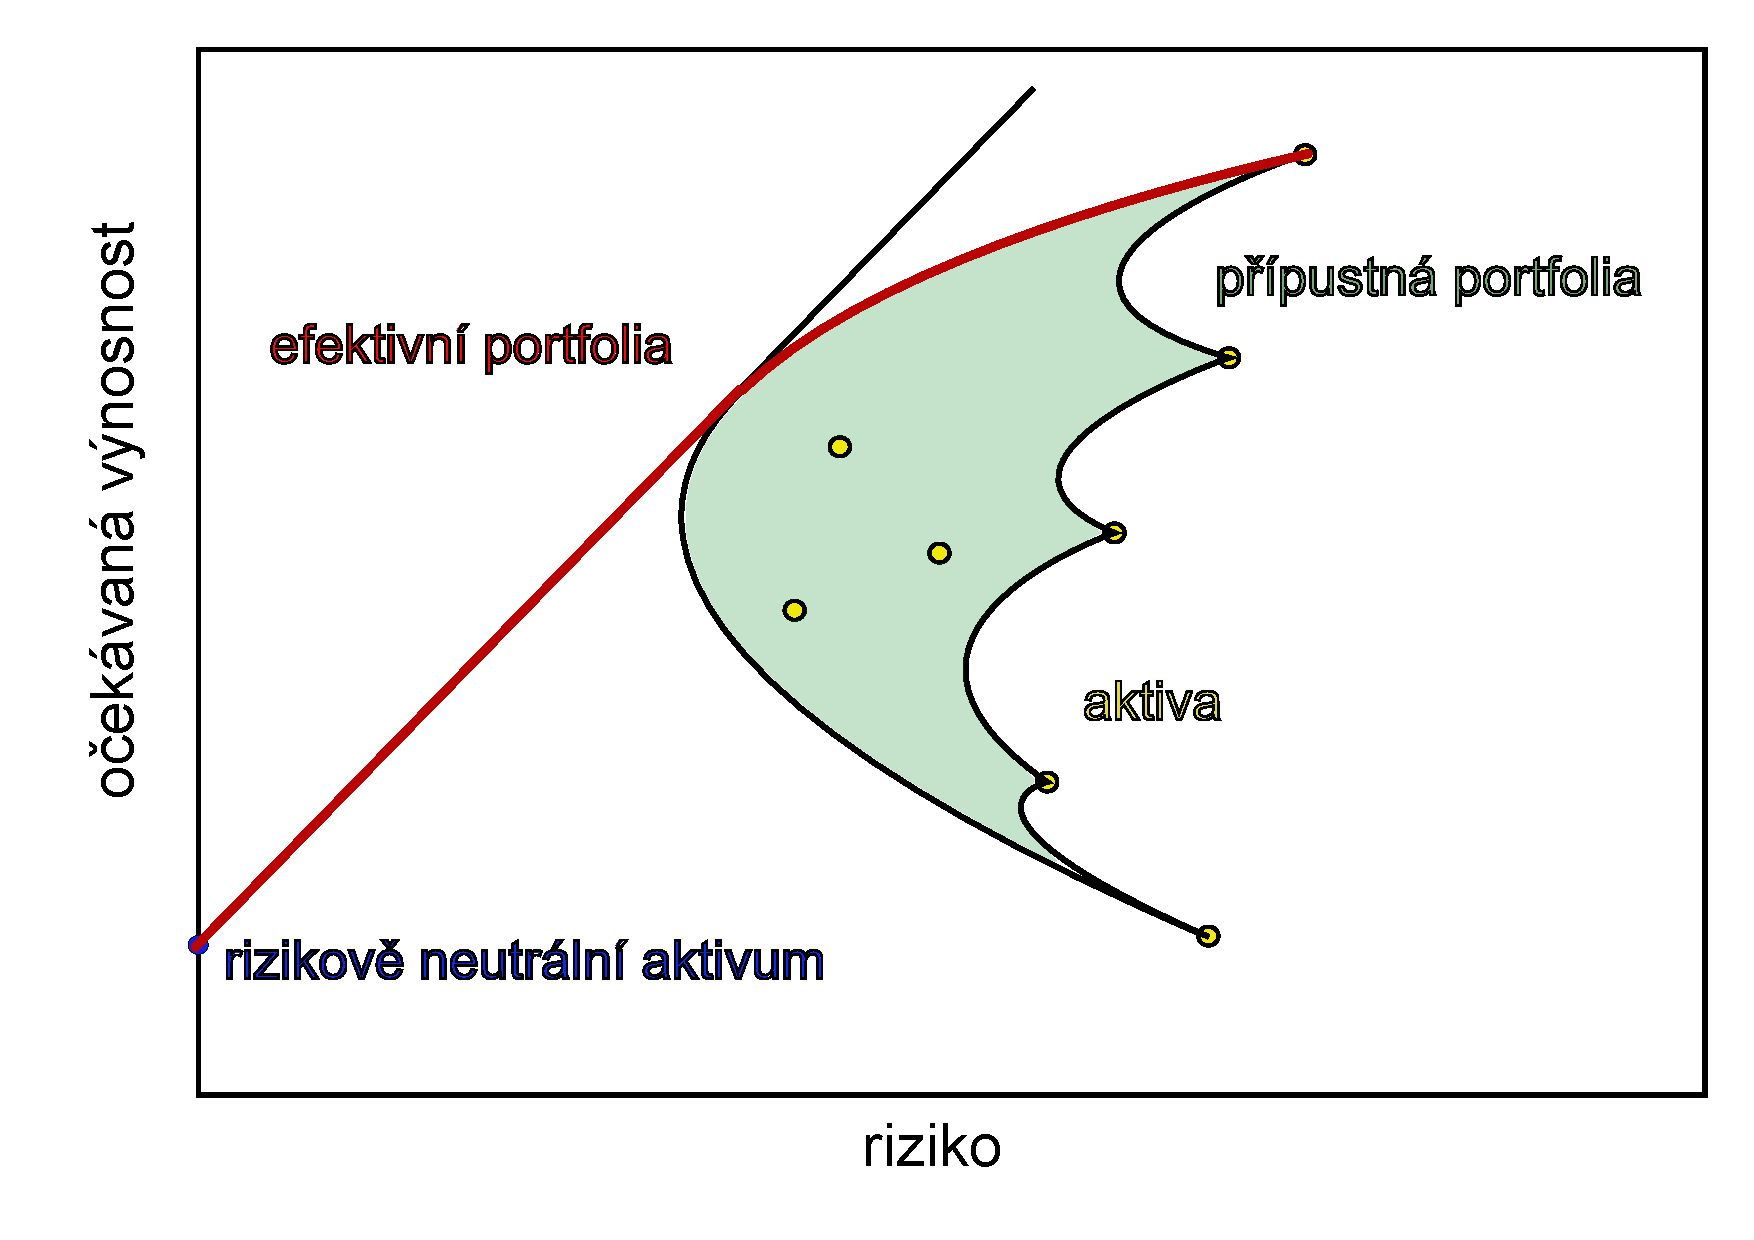
\includegraphics[width=11cm]{IMG/graf_5b.pdf}
  \caption{Tobinův model - množina efektivních portfolií v případě, že není povolen prodej na krátko.}
  \label{obr_Tobin_1}
\end{figure}

\begin{figure}[!htbp]
  \centering 
  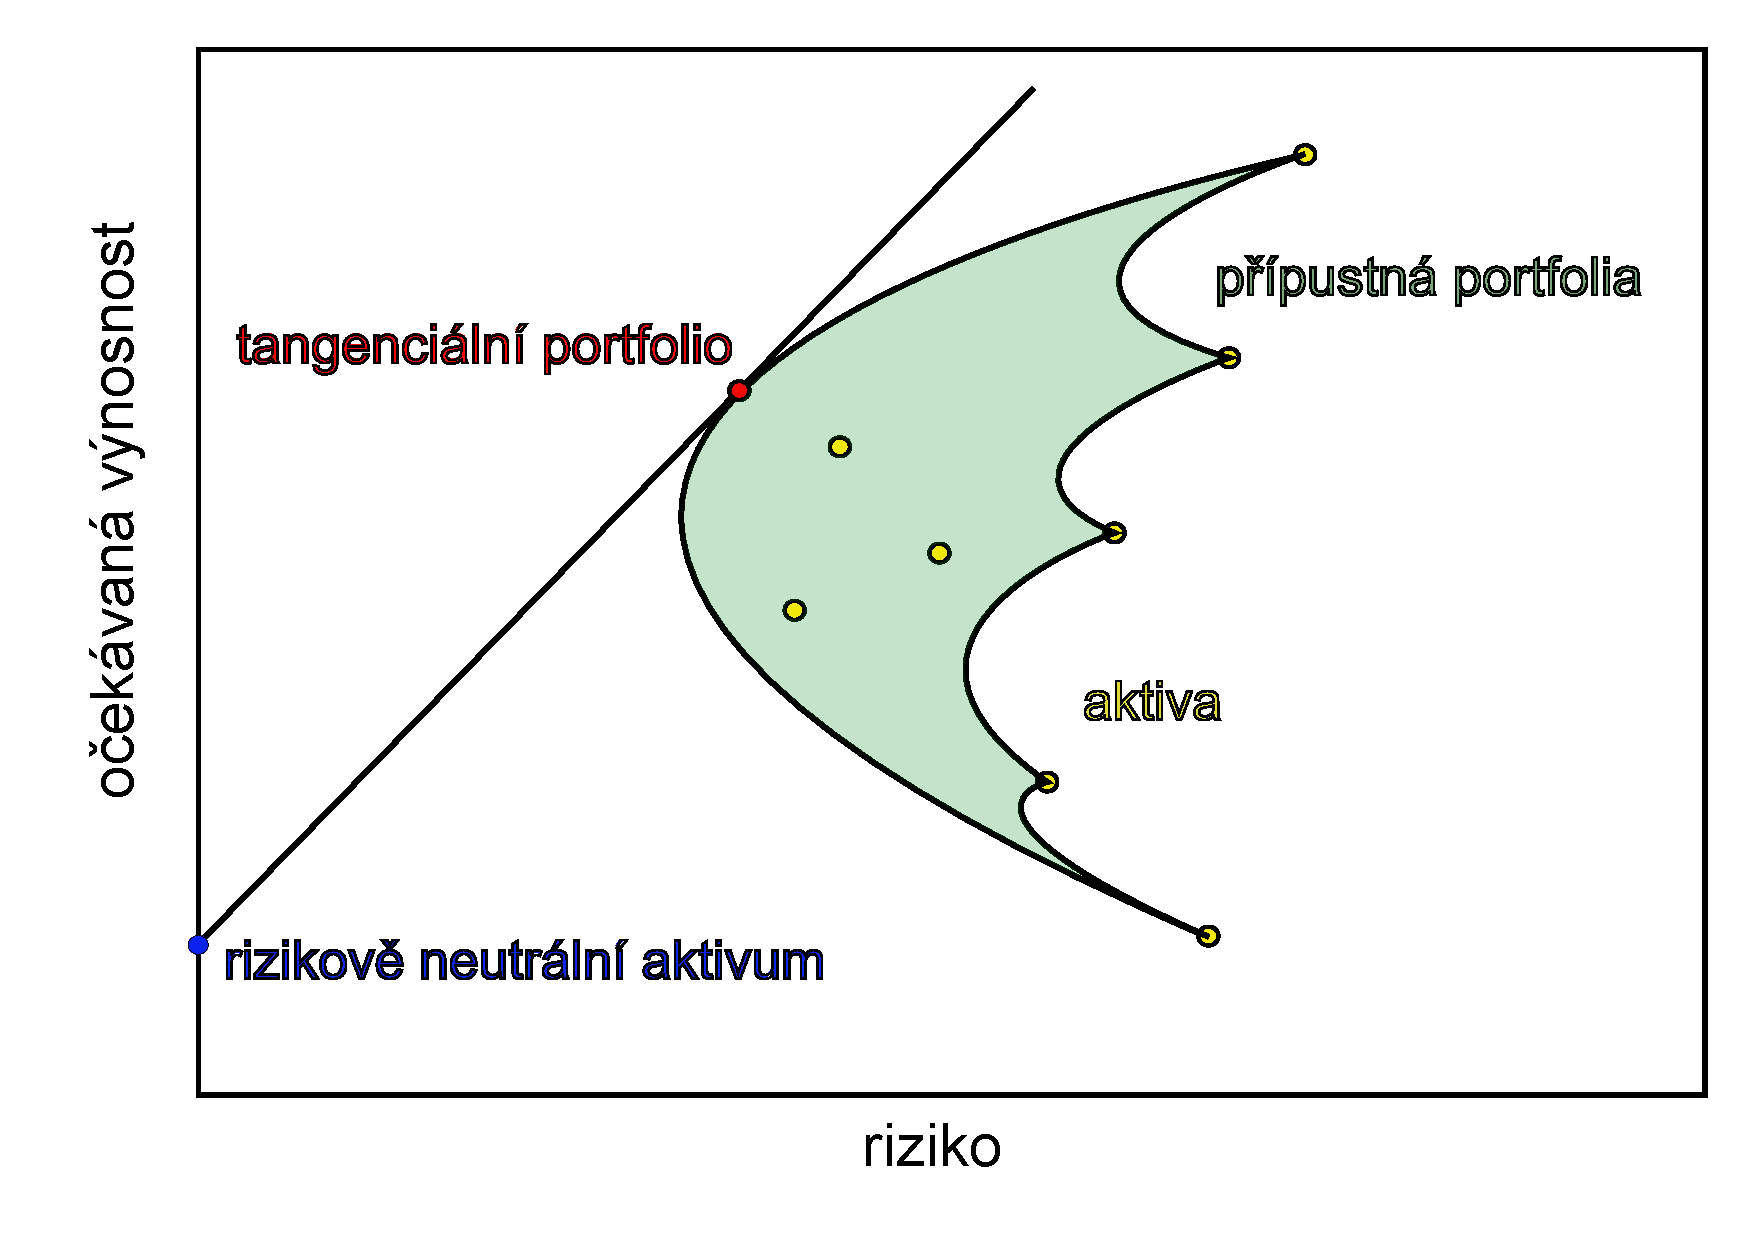
\includegraphics[width=11cm]{IMG/graf_1.pdf}
  \caption{Tobinův model - zobrazení tangenciálního portfolia (rizikového portfolia, do kterého dle Separačního theorému investují všichni investoři při tvorbě optimálního portfolia).}
  \label{obr_Tobin_2}
\end{figure}

%\subsection{Kapitálový model aktiv -- CAPM}\label{kapitola_CAPM}
\textit{Capital Asset Pricing Model} (CAPM) vyvinuli nezávisle na sobě autoři Sharpe \cite{sharpe1964}, Lintner \cite{lintner1965} a Mossin \cite{mossin1966} v letech 1964--1966. CAPM zkoumá chování trhu v případě, že se všichni investoři chovají podle Markowitzovy teorie.
Zároveň vychází z Tobinova modelu, protože zahrnuje bezrizikové aktivum.
CAPM stojí na několika výchozích předpokladech, které se dají shrnout do následujících tří:
\begin{itemize}
\item[-] kapitálový trh je efektivní,
\item[-] investoři při sestavování portfolia využívají Markowitzův přístup,
\item[-] investoři mají homogenní očekávání.
\end{itemize}
Předpoklad homogenity očekávání investorů má za následek, že všichni investoři drží stejné rizikové portfolio.
Optimální portfolia investorů se liší pouze v poměru, v jakém kombinují rizikové portfolio a bezrizikové aktivum v závislosti na svých rizikových preferencích.
Toto shrnuje následující věta.

\begin{veta}(Separační teorém)
Optimální kombinace rizikových cenných papírů může být stanovena bez jakékoliv znalosti investorových postojů k riziku a výnosnosti.
\end{veta}

Předpokládáme-li rovnováhu trhu, bývá tangenciální portfolio nazýváno jako \textit{tržní portfolio}.
Důležitým důsledkem pak je, že váha každého cenného papíru v tržním portfoliu je rovna jeho tržní ceně. \label{vahy_trznihodnota}
Tento poznatek budeme později využívat při konstrukci spojitého rovnovážného modelu.

\subsection{Markowitzova teorie portfolia}\label{Markowitz_kap}

Abychom blíže pochopili pojmy používané v Kapitole \ref{KTP} přiblížíme na tomto místě jejich odvození.

\begin{figure}[!htbp]
  \centering 
  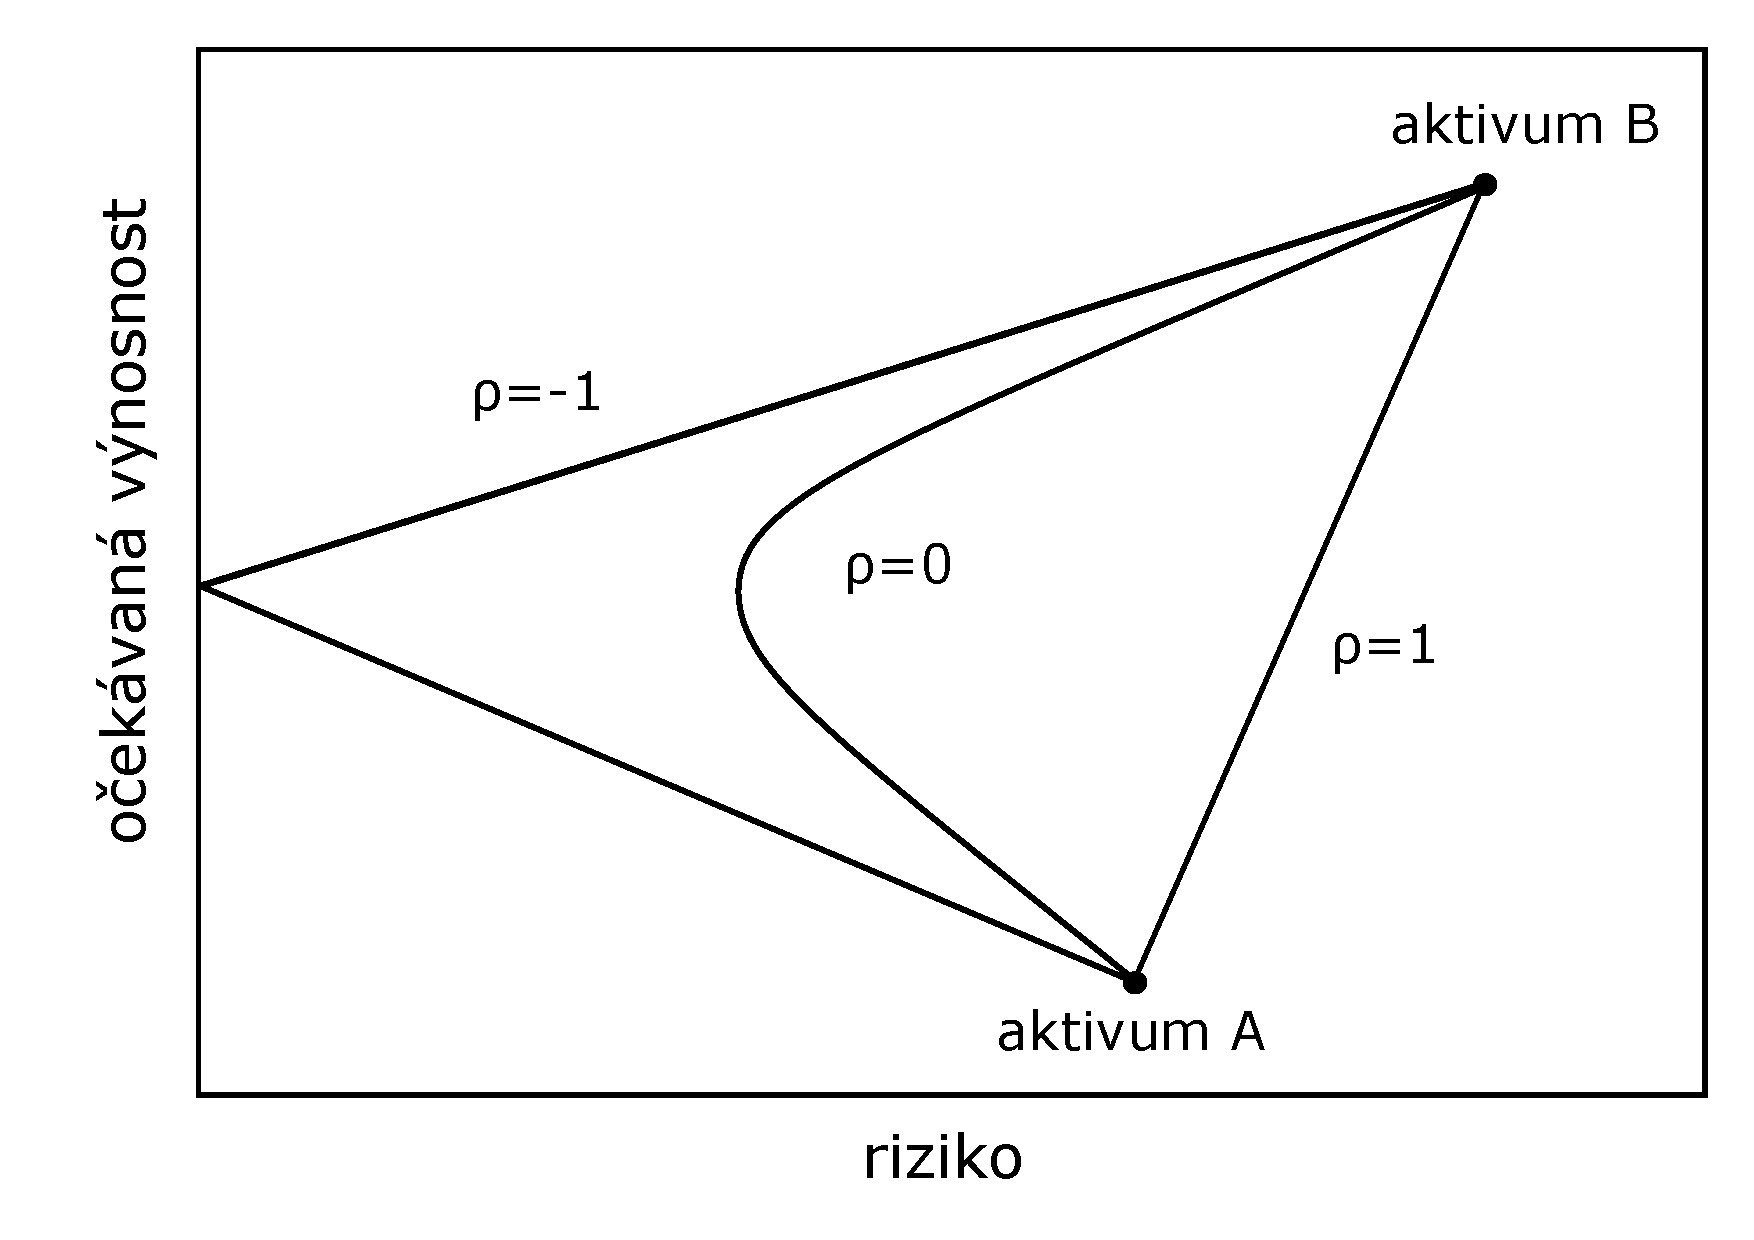
\includegraphics[width=11cm]{IMG/pripustna_portfolia.pdf}
  \caption{Odvození množiny přípustných portfolií  dle Markowitzovy teorie portfolia.}
\end{figure}

%%%%%%%%%%%%%%%%%%%%%%%%{Dynamická teorie portfolia}

\section{Dynamická teorie portfolia}
Hlavní výhodou dynamického modelu pro výběr aktiv v portfoliu je přizpůsobování se měnícím se podmínkám trhu a proto je více realistický než model statický.
Naproti tomu je dynamický model komplikovanější, hůře interpretovatelný a při jeho využití se nevyhneme složitější matematické teorii, kterou je stochastický kalkul.

\begin{comment}
\subsection{Matematický úvod}
Na tomto místě připomeneme některé základní pojmy ze stochastické analýzy a značení obvykle užívané v dynamické teorii portfolia. 

\begin{definice}
Stochastický proces $\{W(t):t\ge0\}$ definovaný na pravděpodobnostním prostoru $(\Omega,\mathcal{A},\mathsf{Pr})$ se nazývá \textit{standardní (jednorozměrný) Wienerův proces} právě tehdy, když jsou splněny následující podmínky
\begin{enumerate}
\item[1.]$W(0)=0$, 
\item[2.]funkce $t\to W(t)$ (trajektorie Wienerova procesu) je spojitá s pravděpodobností jedna,
\item[3.]proces $\{W(t):t\ge0\}$ má nezávislé přírůstky, 
\item[4.]pro všechna $t\ge s\ge0$ jsou přírůstky $W(t)-W(s)$ normálně rozdělené se střední hodnotou nula a rozptylem $t-s$.
\end{enumerate}
Standardní \textit{$n$-rozměrný Wienerův proces} je vektorový stochastický proces
$$\boldsymbol{W}(t) = (W_1(t), \dots, W_n(t))^\mathrm{T}$$
jehož složky $W_k(t)$ jsou nezávislé, standardní jednorozměrné Wienerovy procesy.
\end{definice}
Wienerův proces je stavebním kamenem matematického modelování ve finanční matematice. 
Tento stochastický proces se používá pro popis chování ceny aktiva v čase. 

Budeme předpokládat, že proces popisující vývoj ceny aktiva v čase se řídí následujícím modelem
$$\mathrm{d}P(t)=P(t)\,\mu(t)\,\mathrm{d}t+P(t)\,\sigma(t)\,\mathrm{d}W(t),$$
kde $P(t)$ je cena aktiva v čase $t$, $\mu(t)$ a $\sigma(t)$ jsou stochastické procesy a $W(t)$  je jednorozměrný Wienerův proces.
Tento model předpokládá, že na trhu je pouze jedno rizikové aktivum.

Model pro vývoj ceny aktiv na trhu, který předpokládá existenci $n$ rizikových aktiv je dán jako
$$\mathrm{d}P_j(t)=P_j(t)\,\mu_j(t)\,\mathrm{d}t+P_j(t)\sum_{k=1}^{n}\xi_{jk}(t)\,\mathrm{d}W_k(t),$$
kde $P_j(t)$ je cena aktiva $j$ v čase $t$, $\mu_j(t)$ a $\xi_{jk}(t)$ jsou stochastické procesy a $\boldsymbol{W}(t)=(W_1(t),\dots,W_n(t))^\mathrm{T}$ je $n$-rozměrný Wienerův proces. 
Pro více informací o mnohorozměrných modelech viz \cite{etheridge2002course}.

Chování ceny bezrizikového aktiva je popsáno modelem
$$\mathrm{d}B(t)=B(t)\,r_f(t)\,\mathrm{d}t,$$
kde $B(t)$ je cena bezrizikového aktiva v čase $t$ a $r_f(t)$ je bezriziková úroková míra.
\end{comment}

\subsection{Mertonův model}
První článek zabývající se dynamickou teorií portfolia napsal Robert Carhart Merton v roce 1971 \cite{merton1971}.
Merton předpokládal platnost rovnovážného modelu CAPM a dál tuto teorii rozšířil o spojitý model pro cenu aktiva využívající stochastické procesy.
Přitom ukázal, že zůstává zachována platnost všech závěrů z teorie CAPM, zejména pak separačního teorému.
Což znamená, že bez újmy na obecnosti můžeme uvažovat jen dvě aktiva -- bezrizikové aktivum s mírou výnosnosti $r_f$ a tržní portfolio (které můžeme považovat za jedno rizikové aktivum). 

Merton předpokládá, že hodnota tržního portfolia $P(t)$ se řídí stochastickým procesem
$$\mathrm{d}P(t)=P(t)\,\mu_p\,\mathrm{d}t+P(t)\,\sigma_p\,\mathrm{d}W(t)$$
kde $W(t)$ je jednorozměrný Wienerův proces a $\mu_p$, $\sigma_p$ jsou konstanty. 

V každém čase $t$ vybírá investor své optimální portfolio volbou vah portfolia.
Majetek, který investor investuje do optimálního portfolia v čase $t$, označíme $w(t)$.
Váhu tržního portfolia v optimálním portfoliu označíme $X_p(t)$ a váhu bezrizikového aktiva označíme $X_f(t)=(1-X_p(t))$. 
Proces popisující vývoj investorova majetku je dán jako
$$\frac{\mathrm{d}w(t)}{w(t)}=X_p(t)\,\frac{\mathrm{d}P(t)}{P(t)}+\big(1-X_p(t)\big)\,r_f\,\mathrm{d}t.$$
Merton odvodil explicitní řešení této stochastické diferenciální rovnice za předpokladu, že charakteristiky výnosnosti aktiva jsou konstantní.

Avšak Mertonův spojitý rovnovážný model vykazuje inkonzistenci, což dokázali Ohlson a Rosenberg \cite{ohlson} hned v roce 1976.
Ještě před zveřejněním jejich článku byla uveřejněna ve stejném periodiku Mertonova reakce \cite{merton1975}, ve které hájí své poznatky a poukazuje na jejich nepochopení ze strany oponentů.  
Ohlson a Rosenberg \cite {ohlson} poukazují na rozpor mezi předpokladem, že střední hodnota a rozptyl výnosnosti aktiva jsou konstantní, a předpokladem tržní rovnováhy.
Podrobněji bude tento paradox rozebrán v části \ref{paradox}.


%%%%%%%%%%%%%%%%%%%%%%%%%%{Ohlson-Rosenbergův paradox}
\section{Ohlson-Rosenbergův paradox}\label{paradox}
V této kapitole představíme základní poznatky z článku Ohlsona a Rosenberga \cite{ohlson}, který byl publikován v roce 1976 v \textit{Journal of Financial and Quantitative Analysis}.
Ohlson a Rosenberg jako první poukázali na nekonzistenci Mertonova spojitého modelu \cite{merton1971} spočívající v rozporu předpokladů.

\subsection{Značení a předpoklady}
Na začátek zavedeme značení a  uvedeme základní definice a předpoklady. 
Uvažujme množinu $n$ různých aktiv na daném trhu a označme $\mathcal{T}$ množinu všech uvažovaných časů (diskrétní nebo spojitou).
Nechť $I_t$ značí množinu všech investorů na trhu v čase $t\in \mathcal{T}$.
Cenu aktiva $j$ v čase $t$ označíme $P_j(t)$ a $\boldsymbol{P}(t)=(P_1(t),\dots,P_n(t))^\mathrm{T}$ je vektor cen aktiv v čase $t$.
Analogicky označíme $\boldsymbol{N}(t)=(N_1(t),\dots,N_n(t))^\mathrm{T}$ vektor podílů aktiv v čase $t$.
Potom tržní hodnota aktiva $j$ je rovna $V_j(t)=P_j(t)N_j(t)$.

Míru výnosnosti aktiva $j$, které drží investor v portfoliu v časovém intervalu $(t,t+\Delta t)$ označíme $r_j(t,t+\Delta t)$.
Jak bylo zmíněno výše výnosnost chápeme jako náhodnou veličinu a o její distribuční funkci v čase $t$ vyslovíme tři následující předpoklady:
\begin{enumerate}
\item \label{Stacionarita} \textit{Stacionarita:} distribuční funkce výnosnosti  je stejná ve všech časech $t$,                                                                            
\item \label{Martingalvl} \textit{Markovovská vlastnost:} pro každé $t$ je distribuční funkce výnosnosti nezávislá na všech cenách aktiva pozorovaných před časem~$t$,
\item \label{Homogenita} \textit{Homogenita:} distribuční funkce výnosnosti je stejná pro všechny investory z množiny $I_t$. 
\end{enumerate} 
Tyto předpoklady jsou konzistentní s předpoklady CAPM.

Označme $w_{j}(i,t)$ optimální objem prostředků investovaných do aktiva $j$ investorem $i$ v čase $t$.
Nechť $\boldsymbol{w}(i,t)=(w_{1}(i,t),\dots,w_{n}(i,t))$ představuje optimální alokaci prostředků investora $i$ držených v portfoliu všech aktiv.
Funkce $w_{j}(i,t)$ tedy zohledňuje (rizikové) preference investora $i$ v čase $t$.
  
Nyní můžeme definovat dynamickou tržní rovnováhu jako stav, kdy  nabídka a poptávka jsou v dokonalé rovnováze v každém čase $t$.
Tento stav se také nazývá \textit{vyčištění trhu}.
         
\begin{definice}[Dynamická tržní rovnováha]
Řekneme, že kapitálový trh je v \textit{dynamické rovnováze} právě tehdy, když pro každý čas $t\in \mathcal{T}$, každé podkladové aktivum $j$ a~každého investora $i$ existuje vektor cen aktiv $\boldsymbol{P}(t)$ takový že
$$\sum_{i\in I} w_{j}(i,t)=N_j(t)P_j(t)=V_j(t).$$
Tyto ceny budeme nazývat \textit{rovnovážné ceny}.
\end{definice}

Důsledek Tobinova separačního teorému shrňme jako vlastnost pro prostředky investované do portfolia, kterou budeme dále využívat v~důkazu inkonzistence předpokladů spojitého modelu pro ceny aktiv.
\begin{definice}[Vlastnost separace]\label{vlastnost_separace}
Vektorová funkce pro optimální alokaci investorových prostředků do všech aktiv na trhu $\boldsymbol{w}(i,t)$ respektuje \textit{vlastnost separace} právě tehdy, když existuje vektor $\boldsymbol{X}=(X_1,\dots,X_n)^\mathrm{T}$ takový, že $\sum_{j=1}^nX_j=1$, a existují skalární parametry $\lambda(i,t)$ takové, že
$$\boldsymbol{w}(i,t)=\lambda(i,t)\boldsymbol{X},$$
pro všechny $i\in I$ a všechny $t\in \mathcal{T}$.
\end{definice}
Vlastnost separace \ref{vlastnost_separace} říká, že vektor $\boldsymbol{X}$ představuje váhy tržního portfolia (které se v čase nemění) a parametr $\lambda(i,t)$ zohledňuje rizikové preference investora.

\subsection{Rozpor mezi předpoklady}
Budeme-li předpokládat rovnováhu na trhu a stacionaritu distribuční funkce výnosností, dospějeme ke sporu, jak ukazuje následující věta a důsledek.

\begin{veta} \label{T1}
Nechť $\boldsymbol{P}(t)$ pro všechny $t\in \mathcal{T}$  jsou rovnovážné ceny.
Dále předpokládejme, že na trhu platí vlastnost separace (Definice \ref{vlastnost_separace}).
Pak
\begin{equation}\label{T1_eq}
\mathsf{Pr}\left(\frac{N_j(s)P_j(s)}{N_j(t)P_j(t)}=\frac{N_k(s)P_k(s)}{N_k(t)P_k(t)}\right)=1
\end{equation}
pro všechny časy $s,t\in \mathcal{T}$  a pro každé aktivum $j$ a $k$.
\end{veta}

\begin{proof}
Podle Definice \ref{vlastnost_separace} platí
\begin{equation}\label{CSW}
w_j(i,t)=\lambda(i,t)X_j
\end{equation}
pro všechny časy $t\in \mathcal{T}$, všechny investory $i\in I$ a pro každé aktivum $j$.

Předpoklad dynamické rovnováhy na trhu dává
\begin{equation}\label{E}
\sum_{i\in I} w_{j}(i,t)=N_j(t)P_j(t)
\end{equation}
pro všechny časy $t\in \mathcal{T}$ a pro každé aktivum $j$.

Dosazením vztahu \eqref{CSW} do rovnice \eqref{E} a vzhledem k tomu, že váhy $X_j$ jsou stejné pro všechny investory $i\in I$, dostáváme
$$N_j(t)P_j(t)=\sum_{i\in I}\lambda(i,t)X_j=X_j\sum_{i\in I}\lambda(i,t).$$
Proto platí
$$\frac{N_j(t)P_j(t)}{N_k(t)P_k(t)}=\frac{X_j\sum_{i\in I}\lambda(i,t)}{X_k\sum_{i\in I}\lambda(i,t)}=\frac{X_j}{X_k},$$
což je nezávislé na čase $t$.         
Z tohoto tvrzení zřejmě plyne vztah \eqref{T1_eq}.
\end{proof}

\begin{dusledek}\label{OR_dusledek}
Nechť 
$$r_j(t,t+\Delta t)=\frac{P_j(t+\Delta t)-P_j(t)}{P_j(t)}=\frac{P_j(t+\Delta t)}{P_j(t)}-1.$$
Budeme předpokládat $N_j(t)=N_j$ pro každé aktivum $i$ a všechna $t\in \mathcal{T}$. 
Z~věty \ref{T1} plyne
\begin{align*}
\mathsf{Pr}\left(\frac{P_j(s)}{P_j(t)}=\frac{P_k(s)}{P_k(t)}\right)=1&\Longrightarrow\mathsf{Pr}\left(\frac{P_j(t+\Delta t)}{P_j(t)}=\frac{P_k(t+\Delta t)}{P_k(t)}\right)=1 \\
&\Longrightarrow\mathsf{Pr}\left(r_j(t,t+\Delta t)=r_k(t,t+\Delta t)\right)=1,
\end{align*}
pro všechna $t\in \mathcal{T}$ a pro všechna aktiva $j$ a $k$.
Proto jsou aktiva $j$ a $k$ vzájemně dokonale zastupitelné.
\end{dusledek}
Důsledek \ref{OR_dusledek} vede k degeneraci trhu, což poukazuje na významný rozpor mezi předpoklady.

Ve své době se Ohlson a Rosenberg nesetkali s pochopením.
Důkazem toho je okamžité odmítnutí jejich závěrů ze strany Mertona publikované v článků \cite{merton1975}, kde tvrdí, že rozporu bylo docíleno jen díky nereálným předpokladům. 
Ve skutečnosti reaguje jen na důsledky nikoli na důkaz stěžejní věty článku \cite{ohlson}.  
Za povšimnutí stojí, že Mertonova reakce vychází ještě před samotným článkem Ohlsona a Rosenberga.

%%%%%%%%%%%%%%%%%%%%%%%%%%{Stochastická teorie portfolia}

\section{Stochastická teorie portfolia}
V této kapitole jsou shrnuty některé základní poznatky Stochastické teorie portfolia, která byla inspirací pro studium spojitých modelů v teorii portfolia uvedených v této práci.
Budeme diskutovat o výhodách a nevýhodách tohoto přístupu.

Pojem \textit{Stochastická teorie portfolia} (SPT) zavedl Robert Fernholz ve své monografii \cite{fern}.
Jedná se o matematickou teorii, která zkoumá chování portfolia jakožto i strukturu kapitálového trhu.
Hlavní výhodou oproti klasické teorii portfolia jsou méně  striktní předpoklady, které dovolují konzistentní přístup bez výskytu Ohlson-Rosenbergova paradoxu \cite{ohlson}.

Na rozdíl od Mertonova modelu se v SPT nepředpokládá tržní rovnováha.
Parametry stochastického procesu, kterým se řídí cena aktiva, jsou v SPT také stochastické procesy nikoli konstanty jako v Mertonově přístupu.
Dokonce, na rozdíl od klasického přístupu, se v SPT neklade důraz na předpoklad neexistence tržní arbitráže, přičemž se v práci diskutuje o vlastnosti trhu vedoucí k existenci arbitráže. 

Pro vývoj ceny aktiva Fernholz používá následující spojitý logaritmický model
$$\mathrm{d}\log P_j(t)=\gamma_j(t)\,\mathrm{d}t+\sum_{k=1}^{n}\xi_{jk}(t)\,\mathrm{d}W_k(t),$$
kde $P_j(t)$ je cena aktiva $j$ v čase $t$, $\gamma_j(t)$ a $\xi_{jk}(t)$ jsou stochastické procesy a $\boldsymbol{W}(t)=(W_1(t),\dots,W_n(t))^\mathrm{T}$ je $n$-dimenzionální Wienerův proces. 
Proces $\gamma_j(t)$ se nazývá \textit{míra růstu} a $\xi_{jk}(t)$ se nazývá proces \textit{volatility}.
Míru růstu v logaritmickém modelu je možno odvodit z míry výnosnosti ve standardním modelu a naopak podle následujícího vztahu
$$\mu_j(t)=\gamma_j(t)+\frac12\sum_{k=1}^{n}{\xi_{jk}}^2(t).$$
Robert Fernholz uvádí, že v dlouhém časovém horizontu je chování hodnoty portfolia lépe popsáno mírou růstu než mírou výnosnosti.
Uvažujeme-li kovarianční matici $\boldsymbol{\Sigma}$ výnosností aktiv, pak matice volatilit $\boldsymbol{\xi}$ je definována jako
$$\boldsymbol{\Sigma}=\boldsymbol{\xi}\boldsymbol{\xi}^\mathrm{T}.$$
Tedy $\boldsymbol{\xi}$ je maticová odmocnina z $\boldsymbol{\Sigma}$.

Jedním ze základních pojmů v SPT jsou \textit{portfolio generující funkce}, pomocí nichž jsou tvořeny portfolia, které mají dobře definované výnosnosti. 
Podrobnější informace je možno najít v knize \cite{fern} a článku \cite{kara}.

Studium SPT nás motivovalo k hledání vhodného spojitého modelu pro popis cen aktiv v portfoliu, který rovněž odstraní Ohlson-Rosenbergův paradox a zároveň bude zachovávat platnost poznatků teorie CAPM.
Tento model budeme konstruovat v Kapitole \ref{muj_model}.



%%%%%%%%%%%%%%%%%%%%%%%%%%%%%%%

\section{Paradox v teorii portfolia a Věta o~separaci do~dvou fondů} \label{john}
Nekonzistencí obvyklých předpokladů teorie portfolia se v roce 2009 zabýval také John Stalker profesor na univerzitě v Princetonu. 
V preprintu \cite{john} uvádí algebraický důkaz inkonzistence předpokladů, kde využívá Tobinovu \textit{Větu o~separaci do~dvou fondů}. 
V následujícím textu budou tyto myšlenky rozpracovány.

Uvažujme následující předpoklady obvyklé pro teorii portfolia:
\begin{enumerate}
\item \label{predpoklad_konstantnosti_vynosu_a_rizika} Ceny podkladových aktiv se řídí It\^oovými procesy, které mají konstantní očekávané míry výnosnosti a konstantní kovariance výnosností. 
\item Neexistují žádná omezení na množství aktiv držených investorem. Aktiva jsou navíc nekonečně dělitelná.
\item Neexistují žádné transakční náklady a cena prodeje a nákupu podkladového aktiva se neliší.
\item Investoři se chovají podle Markowitzovy teorie, což znamená, že minimalizují riziko svého portfolia pro dané očekávané míry výnosnosti.
\item \label{predpoklad_hodnost} Na trhu existuje pouze jedno bezrizikové aktivum. Kovarianční matice rizikových aktiv má maximální hodnost.
\item \label{predpoklad_konstantnosti_N} Na trhu existuje rovnováha a každý investor nabízející aktivum najde kupce a naopak.
\end{enumerate}

Dále dokážeme, že tyto předpoklady jsou nekonzistentní pro trh s více než dvěma rizikovými aktivy.
K tomu využijeme Větu o~separaci do~dvou fondů, kterou poprvé dokázal  James Tobin ve svém článku \cite{tobin}. 
Tobin předpokládal platnost předpokladů CAPM a zároveň zahrnul existenci bezrizikového aktiva.
Naproti tomu v knize Williama Sharpeho \cite{sharpe} a v článku Roberta Mertona \cite{merton} najdeme podobné závěry bez předpokladu existence bezrizikového aktiva.
Merton navíc tyto myšlenky zobecňuje pro více než dva fondy \cite{merton1973}.
Podrobnějším rozbor věty o dvou fondech je uveden v knize \cite{cass1970structure}.
\begin{veta}[Věta o~separaci do~dvou fondů]
%Efektivní portfolio každého investora lze získat jako kombinaci dvou fondů.
Optimální portfolio každého investora lze získat jako kombinaci dvou fondů.
\end{veta}
%Efektivní nebo spíš optimální?

Na trhu s~$m$ podkladovými aktivy uvažujme dvě portfolia (neboli dva fondy) a jejich váhy označme $\boldsymbol{a}=(a_1,\dots,a_m)^\mathrm{T}$ a $\boldsymbol{b}=(b_1,\dots,b_m)^\mathrm{T}$. Z těchto dvou fondů pak můžeme sestavit optimální portfolia všech investorů na trhu.
Množinu všech investorů označme $I$ a pro každého investora uvažujme jeho rizikové preference, které určují jeho optimální portfolio, a popišme je pomocí parametrů $\alpha_i(t)$ a $\beta_i(t)$.
Optimální portfolio $i$-tého investora bude zahrnovat $\alpha_ia_j+\beta_ib_j$ množství $j$-té akcie.

Váhy $\boldsymbol{a}$ a  $\boldsymbol{b}$ dvou uvažovaných fondů závisí pouze na očekávaných výnosnostech a riziku podkladových aktiv na trhu, které jsou v čase konstantní dle předpokladu \ref{predpoklad_konstantnosti_vynosu_a_rizika}.
Parametry $\alpha_i(t)$ a $\beta_i(t)$ závisí na individuálních preferencích jednotlivých investorů (např. rizikové preference nebo objem investic) a mohou se lišit.
Tyto preference se mohou v čase měnit a tak parametry mohou záviset i na čase.

Označme $A(t)$ součet všech parametrů $\alpha_i(t)$ pro všechny investory a analogicky $B(t)$ součet parametrů $\beta_i(t)$ .
Tedy $A(t)=\sum_{i\in I}\alpha_i(t)$ a $B(t)=\sum_{i\in I}\beta_i(t)$.
Pak celková hodnota držená všemi investory v $j$-tém aktivu je $Aa_j+Bb_j$ a musí být rovna tržní hodnotě aktiva.
Platí
$$A(t)\,a_j+B(t)\,b_j=P_j(t)\,N_j,$$
kde $P_j(t)$ je tržní cena podkladového aktiva $j$ v čase $t$ a $N_j$ je jeho dostupné množství.
Přičemž $A(t),B(t)$ a $ P_j(t)$ jsou funkce času a $N_j$ je konstantní v~čase podle předpokladu \ref{predpoklad_konstantnosti_N}.
Pro změnu ceny aktiva $j$ mezi časem $t$ a časem $t+\Delta t$ platí
\begin{displaymath}
\Delta P_j = \frac{a_j}{N_j}\Delta A + \frac{b_j}{N_j}\Delta B,
\end{displaymath}
kde $\Delta A = A(t+\Delta t) - A(t)$ and $\Delta B = B(t+\Delta t)- B(t)$.

Uvažujme míru výnosnosti podkladového aktiva $j$ za čas $\Delta t$
\begin{displaymath}
r_j(t,t+\Delta t)=\frac{\Delta P_j}{P_j(t)}=\frac{a_j}{N_jP_j(t)}\Delta A + \frac{b_j}{N_jP_j(t)}\Delta B
\end{displaymath}
a kovarianční matici výnosností podkladových aktiv držených v portfoliu
$$\boldsymbol{\Sigma}(\boldsymbol{r})=
\begin{pmatrix}
\mathsf{D}(r_1)  & \ldots & \mathsf{C}(r_1,r_m)  \cr \vdots & \ddots & \vdots\cr \mathsf{C}(r_m,r_1)   & \ldots & \mathsf{D}(r_m) 
\end{pmatrix}.$$
Vzhledem k vlastnostem kovariance (viz \cite{andel}) můžeme kovarianční matici výnosností rozložit na součin 
$$
%\begin{displaymath}
\boldsymbol{\Sigma}(\boldsymbol{r})= 
\begin{pmatrix}
\frac{a_1}{N_1P_1} & \frac{b_1}{N_1P_1}\cr \vdots & \vdots\cr \frac{a_m}{N_mP_m} & \frac{b_m}{N_mP_m}
\end{pmatrix}
%\end{displaymath}
\times
%\begin{displaymath*}
\begin{pmatrix}
\frac{\mathsf{C}(\Delta A, \Delta A)}{\Delta t} &
\frac{\mathsf{C}(\Delta A, \Delta B)}{\Delta t} \cr
\frac{\mathsf{C}(\Delta B, \Delta A)}{\Delta t} & \frac{\mathsf{C}(\Delta B,
\Delta B)}{\Delta t} 
\end{pmatrix}
%\end{displaymath*}
\times
%\begin{displaymath*}
\begin{pmatrix}
\frac{a_1}{N_1P_1} & \ldots & \frac{a_m}{N_mP_m}\cr \cr \frac{b_1}{N_1P_1} & \ldots &
\frac{b_m}{N_mP_m}
\end{pmatrix}.
%\end{displaymath*}
$$

Dále platí, že hodnost součinu matic je menší nebo rovna maximální z hodností matic jeho činitelů.
Vzhledem k tomu nemůže mít kovarianční matice výnosností podkladových aktiv držených v portfoliu hodnost větší než dvě.
Avšak to je v rozporu z předpokladem \ref{predpoklad_hodnost}, pokud uvažujeme portfolio s více než dvěma podkladovými aktivy.

%%%%%%%%%%%%%%%%%%%%%%%%%%%%%%%

\section{Spojitý rovnovážný model s očekávanou výnosností závislou na ceně aktiva }\label{muj_model}
V Kapitolách \ref{paradox} a \ref{john} jsme ukázali, že v teorii portfolia běžně používaný dynamický model není konzistentní.
Proto se chceme pokusit navrhnout takový model, který by nebyl touto inkonzistencí předpokladů zatížen.
Uvažujme spojitý model, který bude mít méně omezující předpoklady než model Mertonův.
Model, který předkládáme v této kapitole, předpokládá rovnováhu na trhu, nicméně očekávaná míra výnosnosti není konstantní v čase.

Na základě poznatků z teorie portfolia budeme hledat vztah mezi očekávanou výnosností a cenou aktiva, který bychom mohli použít v modelu.
Nechť $\boldsymbol{P}$ je vektor cen $n$ podkladových aktiv.
Předpokládejme, že tyto ceny se řídí následující soustavou stochastických diferenciálních rovnic, pro $j=1,\dots,n$ platí
\begin{equation} \label{SDE}
\mathrm{d}P_j(t)=P_j(t)\mu_j(t)\,\mathrm{d}t+P_j(t)\sum_{k=1}^{n}\xi_{jk}(t)\,\mathrm{d}W_k(t),
\end{equation}
kde $\boldsymbol{W}(t)=(W_1(t),\dots,W_n(t))^\mathrm{T}$ je $n$-rozměrný Wienerův proces, $\mu_j(t)$ je očekávaná míra výnosnosti podkladového aktiva $j$ a $\xi_{jk}(t)$ je proces volatility podkladových aktiv $j$ a $k$. 
Pro zjednodušení předpokládejme, že výnosnost bezrizikového aktiva $r_f=0$.
Nechť $\boldsymbol{X}=(X_1,\dots,X_n)^\mathrm{T}$ je vektor vah v tržním portfoliu, který je dán jako
\begin{equation} \label{vahy}
\boldsymbol{X}=\frac{\boldsymbol{\Sigma}^{-1}\boldsymbol{\mu}}{\boldsymbol{1}^\mathrm{T}\,\boldsymbol{\Sigma}^{-1}\boldsymbol{\mu}},
\end{equation}
kde $\boldsymbol{1}$ je vektor jedniček, $\boldsymbol{\mu}=(\mu_1,\dots,\mu_n)^\mathrm{T}$ je vektor očekávaných výnosností podkladových aktiv a $\boldsymbol{\Sigma}$ je kovarianční matice výnosností podkladových aktiv (viz \cite{fabozzi}).

Uvažujme o řešitelnosti a počtu řešení soustavy rovnic \eqref{vahy} vzhledem k~$\boldsymbol{\mu}$.
Soustavu upravíme do tvaru
\begin{equation} \label{hodnost}
\left(\boldsymbol{X}\boldsymbol{1}^\mathrm{T}-\mathbf{I}\right)\boldsymbol{\Sigma}^{-1}\boldsymbol{\mu}=0.
\end{equation}
Podle předpokladů v teorii portfolia zmíněných v Kapitole \ref{john} je kovarianční matice plné hodnosti, tedy i matice $\boldsymbol{\Sigma}^{-1}$ má hodnost $n$.
Naproti tomu, díky předpokladu $\sum_{j=1}^nX_j=1$, má matice $\left(\boldsymbol{X}\boldsymbol{1}^\mathrm{T}-\mathbf{I}\right)$ lineárně závislé řádky, jelikož
součet libovolných $n-1$ řádků matice  je roven zbývajícímu řádku vynásobenému minus jednou.
Dá se tedy dokázat, že tato matice má hodnost $n-1$.
To znamená, že soustava rovnic \eqref{hodnost} má nekonečně mnoho řešení vzhledem k $\boldsymbol{\mu}(t)$.
%Dále hledejme nějaké partikulární řešení této soustavy rovnic.

Jak jsme ukázali v Kapitole \ref{vahy_trznihodnota}, váhy tržního portfolia se rovnají relativním tržním hodnotám podkladových aktiv v tržním portfoliu, tedy
\begin{equation} \label{market_value}
\boldsymbol{X}=\frac{\boldsymbol{V}}{\boldsymbol{1}^\mathrm{T}\,\boldsymbol{V}},
\end{equation}
kde $\boldsymbol{V}$ je vektor tržních hodnot podkladových aktiv na trhu.
Připomeňme, že tržní hodnota aktiva $j$ je dána jako $V_j(t)=P_j(t)N_j(t)$.
Vzhledem ke vztahu mezi tržní hodnotou aktiva a cenou aktiva a vzhledem ke vztahům \eqref{vahy} a \eqref{market_value} můžeme předpokládat, že očekávané výnosnosti $\boldsymbol{\mu}(t)$ jsou funkcemi cen aktiv $\boldsymbol{P}(t)$. 

%Ze vztahů \eqref{vahy} a \eqref{market_value} dostáváme $\boldsymbol{V}=\boldsymbol{\Sigma}^{-1}\boldsymbol{\mu}$ a proto očekávané výnosnosti můžeme vyjádřit jako
%\begin{equation} \label{mu}
%\boldsymbol{\mu}=\boldsymbol{\Sigma}\boldsymbol{V}.
%\end{equation}

%Při zohlednění vztahu \eqref{market_value} dostaneme obecné řešení soustavy rovnic \eqref{hodnost} jako $\boldsymbol{\mu}=k(t)\boldsymbol{\Sigma}\boldsymbol{V}$, kde $k(t)$ je parametrická funkce. %$k\in\mathbb{R}$ je parametr. 
%Což znamená, že nemůžeme najít jednoznačné vyjádření pro vektor $\boldsymbol{\mu}$, ale našli jsme vztah mezi složkami tohoto vektoru. %a k jeho vyjádření nám postačí jeden parametr.

Hledejme vhodné stochastické procesy, které by popisovaly chování vektoru $\boldsymbol{\mu}(t)$.
Pro tento účel rozdělme proces očekávané výnosnosti aktiv na dvě složky.
První složka určuje relativní vztahy mezi jednotlivými očekávanými výnosnostmi aktiv v portfoliu, druhá složka popisuje výnosnost celého trhu dynamicky se měnící v čase.  
Mezi těmito složkami bude platit multiplikativní vztah
\begin{equation} \label{vynos}
\boldsymbol{\mu}(t) =\tilde{\boldsymbol{\mu}}(t)\cdot \mu_M(t)
\end{equation}
kde
vektorový stochastický proces $\tilde{\boldsymbol{\mu}}(t)=(\tilde{\mu}_1(t),\dots,\tilde{\mu}_n(t))^\mathrm{T}$ zachycuje relativní vztahy aktiv v~portfoliu, které se mohou v čase měnit, a
$\mu_M(t)$ je skalární stochastický proces, který charakterizuje dynamiku trhu a nezávisí na volbě konkrétního aktiva.
Dále nechť pro všechny uvažované časy $t$ platí $\sum_{i=1}^n\tilde{\mu}_i(t)=1$.
Pak podle teorie CAPM platí 
\begin{equation} \label{vahy_mu}
\tilde{\boldsymbol{\mu}}(t)=\boldsymbol{X}(t),
\end{equation}
kde $\boldsymbol{X}(t)$ je vektor vah v tržním portfoliu v čase $t$.

Výnosnost celého trhu nevykazuje exponenciální růst, ale pohybuje se přibližně v nějakém intervalu. 
V delším časovém horizontu se projevuje tendence navracet se k průměrné hodnotě.
Proto budeme předpokládat, že míra výnosnosti trhu $\mu_M(t)$ se řídí Vašíčkovým modelem z Kapitoly \ref{Vasickuv_model}
\begin{equation} 
\mathrm{d}\mu_M(t)=\kappa(\theta-\mu_M(t))\,\mathrm{d}t+\sigma\,\mathrm{d}W(t),
\end{equation}
kde $\kappa$, $\theta$ a $\sigma$ jsou konstanty.

Předpokládejme nyní, že uvažovaná podkladová aktiva jsou nekorelovaná, tedy matice $\boldsymbol{\Sigma}$ je diagonální.
Příkladem takových aktiv by mohly být akcie podniků z velmi odlišných odvětví.
Další zjednodušující předpoklady, které pro tuto chvíli zavedeme, bude neměnnost rizika aktiv $\sigma_j=\xi_{jj}$ v průběhu času a také hodnoty aktiv $N_j$ nechť jsou v čase konstantní.

Dosadíme-li vztahy \eqref{vynos} a \eqref{vahy_mu} do stochastické diferenciální rovnice \eqref{SDE}, pak s ohledem na předpoklady učiněné výše dostáváme
\begin{equation}  \label{SDE_cen_diag}
\mathrm{d}P_j(t)=P_j(t)\left(\frac{P_j(t)N_j}{\sum_{i=1}^n P_i(t)N_i}\, \mu_M(t)\right)\,\mathrm{d}t+P_j(t)\sigma_{j}\,\mathrm{d}W_j(t).
\end{equation}

\begin{comment}
Připomeňme, že tržní hodnota  $V_j(t)=P_j(t)N_j(t)$ a $\sigma_{j}=\xi_{jj}$.
Dosadíme-li vztahy \eqref{mu} do stochastické diferenciální rovnice \eqref{SDE}, pak s ohledem na předpoklady učiněné výše dostáváme
$$ 
\mathrm{d}P_j(t)=P_j^2(t){\sigma_{j}}^2N_j\,\mathrm{d}t+P_j(t)\sigma_{j}\,\mathrm{d}W_j(t).
$$
\hrulefill 
Dále budeme hledat vztah pro očekávané hodnoty cen podkladových aktiv.
Ze SDR \eqref{SDE} plyne
\begin{equation}
\mathsf{E}\big(\mathrm{d}P_j(t)\big)=\mathsf{E}\big(P_j^2(t){\sigma_{j}}^2N_j\,\mathrm{d}t+P_j(t)\sigma_{j}\,\mathrm{d}W_j(t)\big)=\mathsf{E}\big(P_j^2(t){\sigma_{j}}^2N_j\,\mathrm{d}t\big),
\end{equation}
protože z vlastností Wienerova procesu máme $\mathsf{E}\big(\mathrm{d}W_j(t)\big)=0$.
Čímž se stochastická diferenciální rovnice zjednodušuje na obyčejnou diferenciální rovnici (ODR), která je řešitelná pomocí separace proměnných.
\begin{align} 
{\mathrm{d}\mathsf{E}\big(P_j(t)\big)}&={\sigma_{j}}^2N_j\,\mathsf{E}\big(P_j^2(t)\big)\mathrm{d}t \notag\\
&={\sigma_{j}}^2N_j\big[\mathsf{D}\big(P_j(t)\big)+\mathsf{E}^2\big(P_j(t)\big)\big]\mathrm{d}t \notag\\
&={\sigma_{j}}^2N_j\big[{\sigma_{j}}^2+\mathsf{E}^2\big(P_j(t)\big)\big]\mathrm{d}t \label{ODE}
\end{align}  
Řešení ODR $\eqref{ODE}$ je
\begin{equation} 
\mathsf{E}\big(P_j(t)\big)=\sigma_j\mathrm{tan}\big({\sigma_j}^3N_jt\big).
\end{equation}
Docházíme tedy k závěru, že řešení má singularitu v konečném čase.
Jelikož pro ${\big(\sigma_j}^3N_jt\big)\to\frac\pi2$ platí $\mathsf{E}\big(P_j(t)\big)\to\infty$. 
To by mohlo být interpretováno jako chování cenových bublin na trhu.
K těm dochází v případě, že investoři ve velkém měřítku investují do aktiv s nadsazenými cenami, což vede k dalšímu umělému zvyšování cen. 
Takový stav nevyhnutelně vede k nečekanému krachu ceny (tzv. prasknutí bubliny).
Problematické je takovou bublinu na trhu poznat, jelikož jsme schopni ji identifikovat až zpětně při extrémním poklesu cen, který je důsledkem mohutného odprodeje aktiv.

V další části představíme model s méně přísnými předpoklady.
Připusťme nyní možnost závislosti mezi jednotlivými aktivy, tedy nechť matice $\boldsymbol{\Sigma}$ není diagonální.
Za těchto předpokladů dosaďme vztah \eqref{mu} do SDR \eqref{SDE}, čímž obdržíme
\begin{equation*} 
 \mathrm{d}P_j(t)=P_j(t)\sum_{k=1}^{n}P_k(t)N_k(t)\sigma_{jk}\,\mathrm{d}t+P_j(t)\sum_{k=1}^{n}\xi_{jk}(t)\,\mathrm{d}W_k(t).
\end{equation*}
Budeme-li opět uvažovat očekávanou hodnotu  cen podkladových aktiv dostáváme vztah
\begin{equation*} 
\mathsf{E}\big( \mathrm{d}P_j(t)\big)=\mathsf{E}\left(P_j(t)\sum_{k=1}^{n}P_k(t)N_k(t)\sigma_{jk}\,\mathrm{d}t\right),
\end{equation*}
z něhož dostaneme následující soustavu obyčejných diferenciálních rovnic
\begin{align*}
\mathrm{d}\mathsf{E}\big(P_j(t)\big)&=N_j\left[\sum_{k=1}^{n}{\sigma_{jk}}^2+\mathsf{E}\big(P_j(t)\big)\sum_{k=1}^{n}\sigma_{jk}\mathsf{E}\big(P_k(t)\big)\right]\mathrm{d}t.
\end{align*}  
Avšak tato soustava je nelineární a bohužel neexistuje její analytické řešení.
Neobejdeme se tedy bez použití numerických metod.
\hrulefill 
\end{comment}

V další části představíme model s méně přísnými předpoklady.
Připusťme nyní možnost závislosti mezi jednotlivými aktivy, tedy nechť matice $\boldsymbol{\Sigma}$ není diagonální.
Zachováme předpoklad konstantnosti volatilit aktiv $\xi_{jk}$ v čase.
Za těchto předpokladů dosaďme vztah \eqref{vynos} a \eqref{vahy_mu} do SDR \eqref{SDE}, čímž obdržíme
\begin{equation} \label{SDE_cen}
 \mathrm{d}P_j(t)=P_j(t)\left(\frac{P_j(t)N_j}{\sum_{i=1}^n P_i(t)N_i}\, \mu_M(t)\right)\,\mathrm{d}t+P_j(t)\sum_{k=1}^{n}\xi_{jk}\,\mathrm{d}W_k(t).
\end{equation}

Často nás více než trajektorie cen podkladových aktiv zajímají očekávané hodnoty cen těchto aktiv.
%\eqref{SDE_cen_diag}
Vztahy pro očekávané hodnoty cen aktiv odvoďme ze soustavy SDR \eqref{SDE_cen}.
Připomeňme, že z vlastností Wienerova procesu, uvedených v definici \ref{WP_def}, plyne, že $\mathsf{E}\big(\mathrm{d}W_j(t)\big)=0$.
\\
\textcolor{red}{???Nekorelovanost $P_j(t)$ a $\mathrm{d}W_j(t)$???}
\\
Pak
\begin{align*}%\label{ODE_cen_ocek}
\mathsf{E}\big( \mathrm{d}P_j(t)\big)&	=\mathsf{E}\left(\frac{P_j^2(t)N_j}{\sum_{i=1}^n P_i(t)N_i}\, \mu_M(t)\,\mathrm{d}t+P_j(t)\sum_{k=1}^{n}\xi_{jk}\,\mathrm{d}W_k(t)\right)\\
&=\mathsf{E}\left(\frac{P_j^2(t)N_j}{\sum_{i=1}^n P_i(t)N_i}\, \mu_M(t)\,\mathrm{d}t\right)
\end{align*}
Čímž se soustava stochastických diferenciálních rovnic zjednodušuje na soustavu obyčejných diferenciálních rovnic
\\
\textcolor{red}{???jde následující rovnice upravit na ODR???}
\\
\begin{align*}
\mathrm{d}\mathsf{E}\big(P_j(t)\big)&=\mathsf{E}\left(\frac{P_j^2(t)N_j}{\sum_{i=1}^n P_i(t)N_i}\, \mu_M(t)\right)\,\mathrm{d}t.
\end{align*}
Avšak tato soustava je nelineární a neexistuje její analytické řešení, proto se neobejdeme bez použití numerických metod.

\begin{figure}[!htbp]
  \centering 
	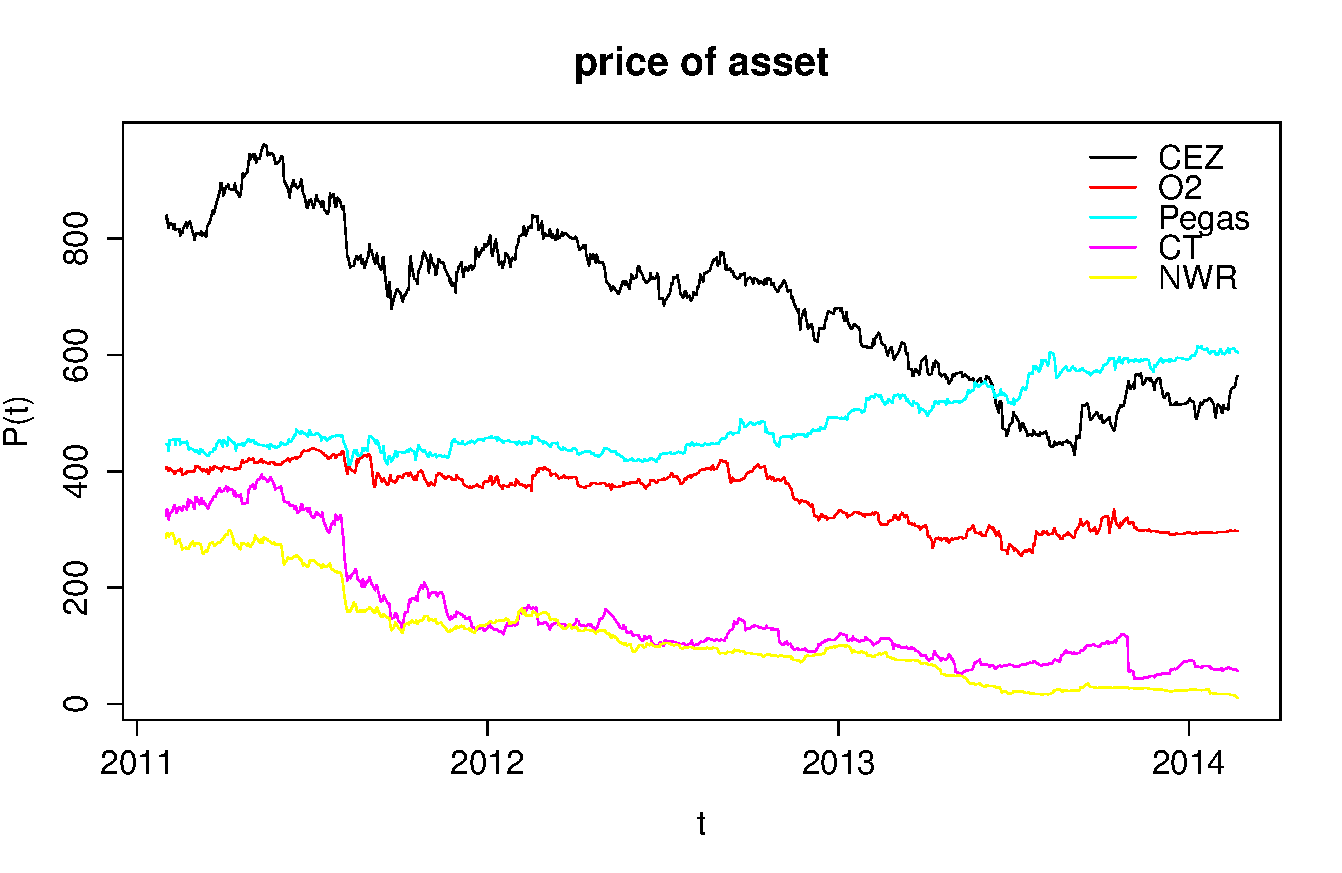
\includegraphics[width=13.5cm, clip, trim= 0 15 25 50]{IMG/data_price_of_asset_ostatni.pdf}\\[5mm]
	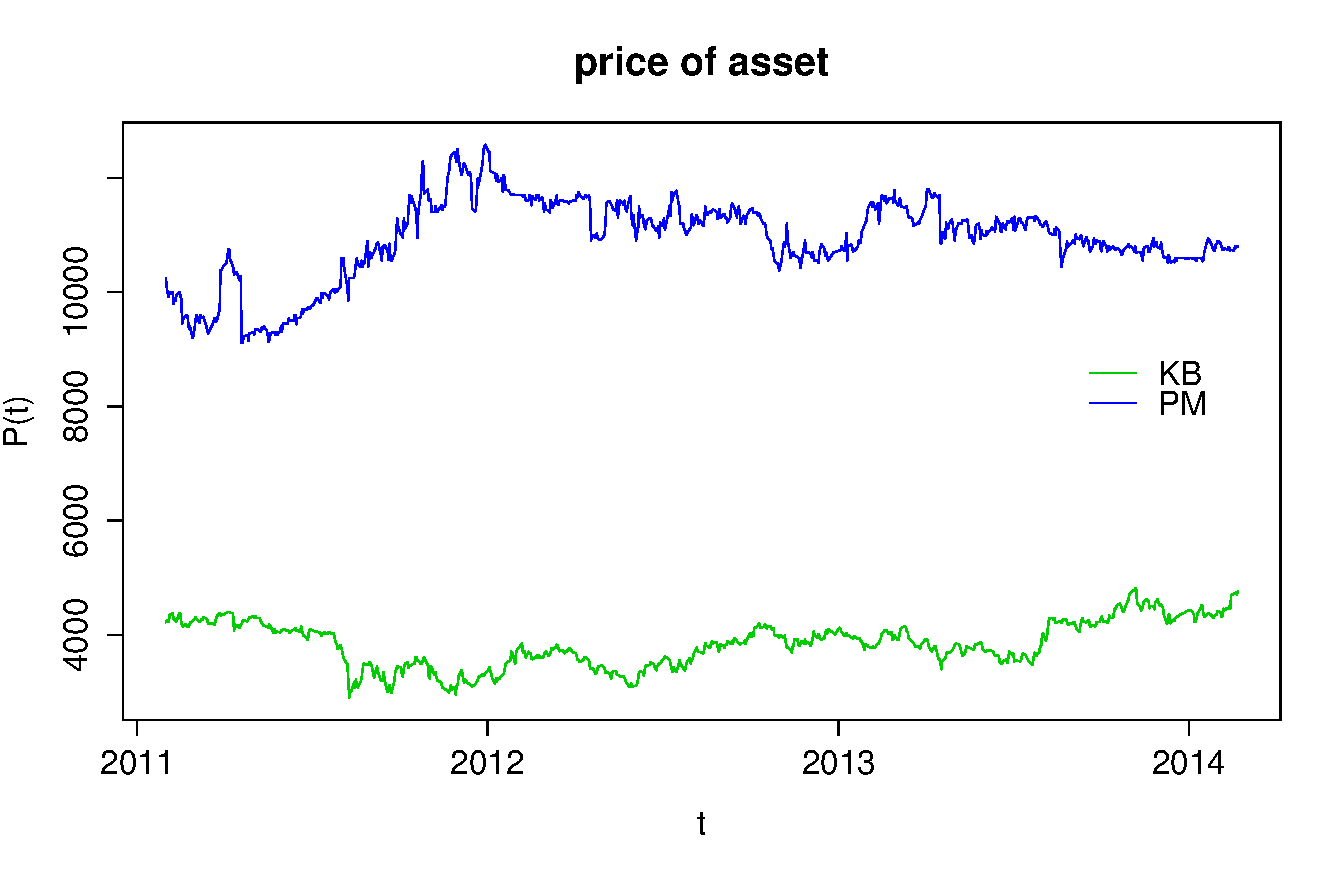
\includegraphics[width=13.5cm, clip, trim= 0 15 25 50]{IMG/data_price_of_asset_KBPM_v2.pdf}	
  \caption{Ceny aktiv v portfoliu}  \label{model_price_of_asset}
\end{figure}

\begin{figure}[!htbp]
  \centering 
	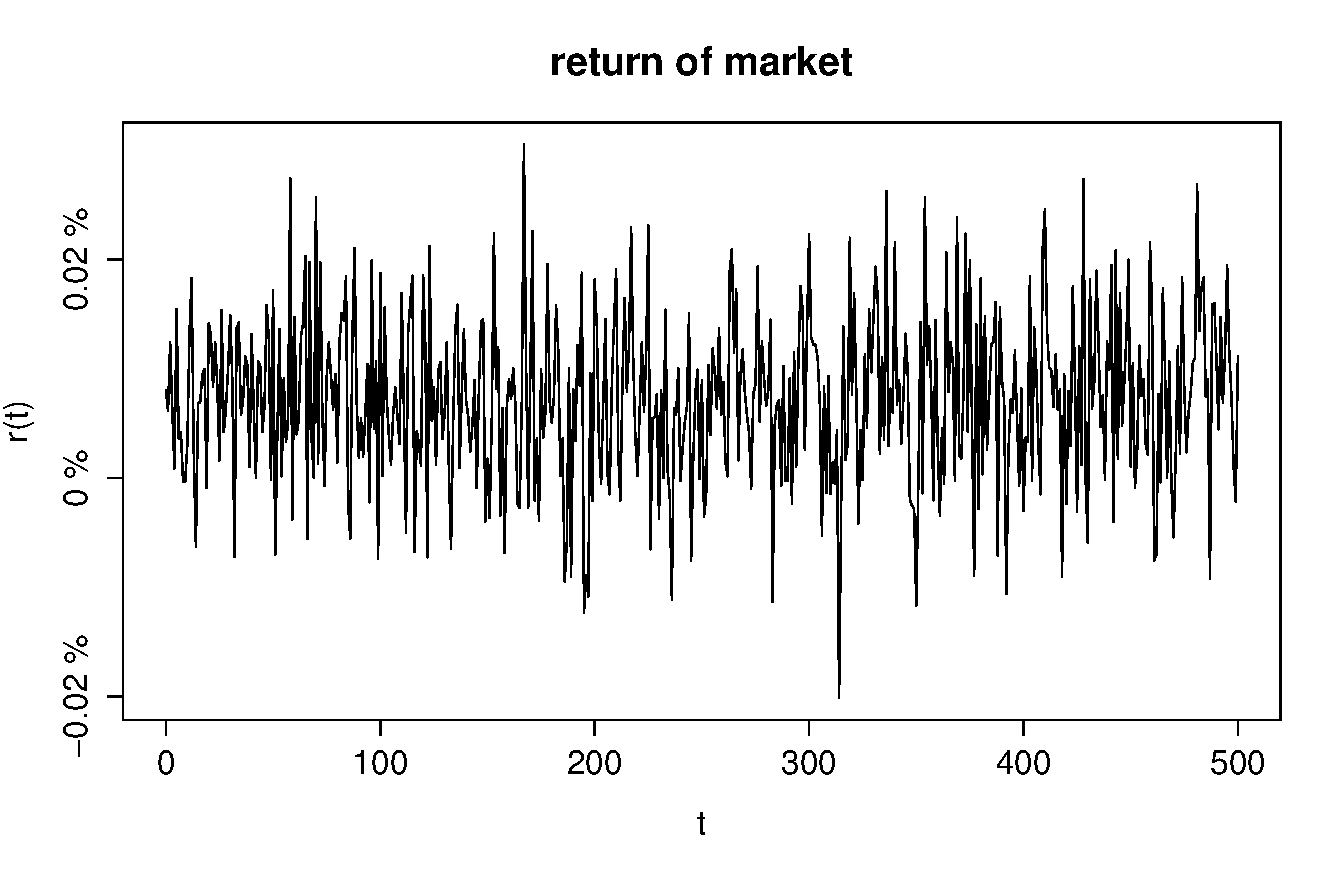
\includegraphics[width=13.5cm, clip, trim= 0 15 25 50]{IMG/return_of_market_v4b.pdf}
  \caption{Model výnosnosti trhu $r(t)$}  \label{return_of_market}
\end{figure}

\begin{figure}[!htbp]
  \centering 
	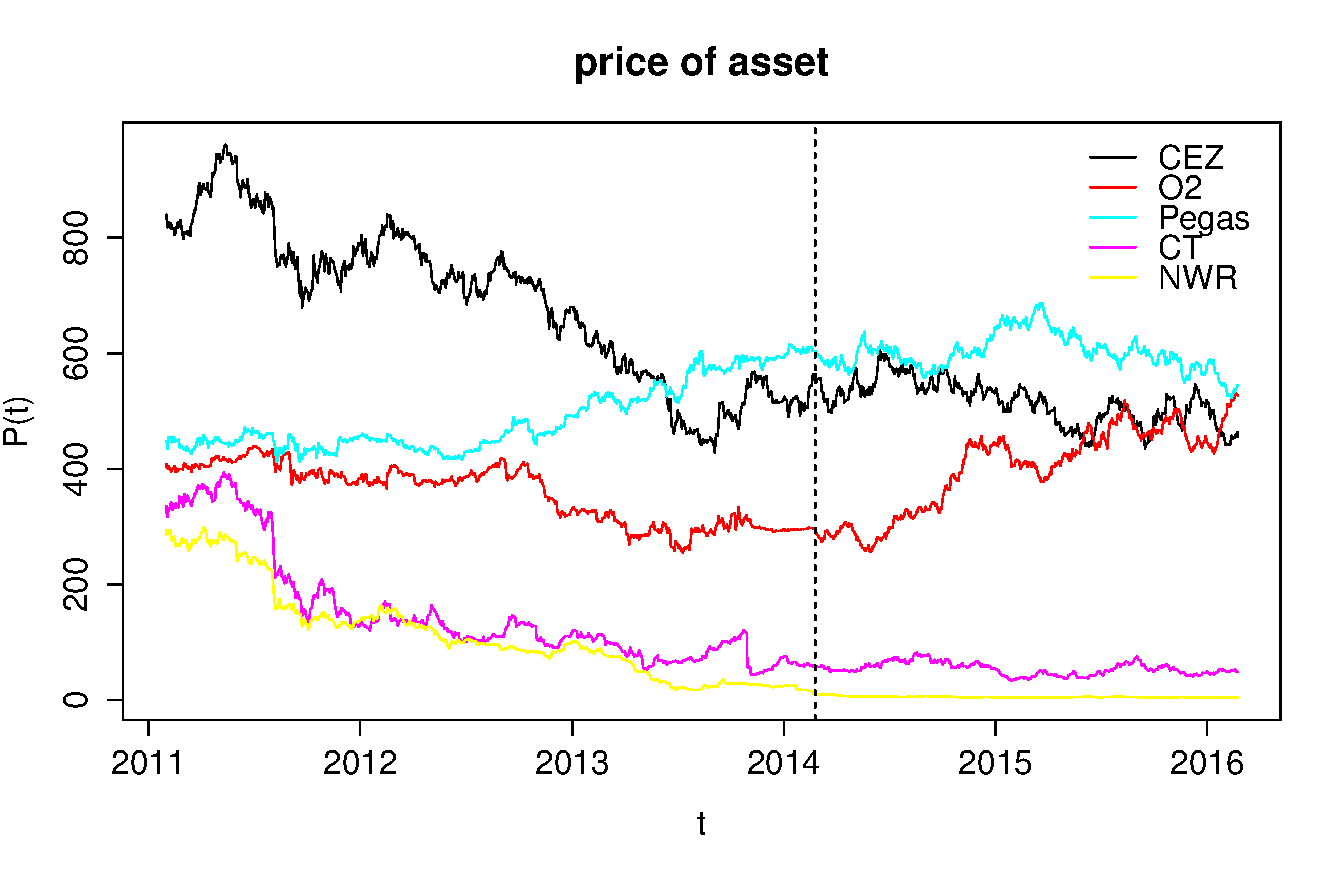
\includegraphics[width=13.5cm, clip, trim= 0 15 25 50]{IMG/ds_price_of_asset_ostatni.pdf}\\[5mm]
	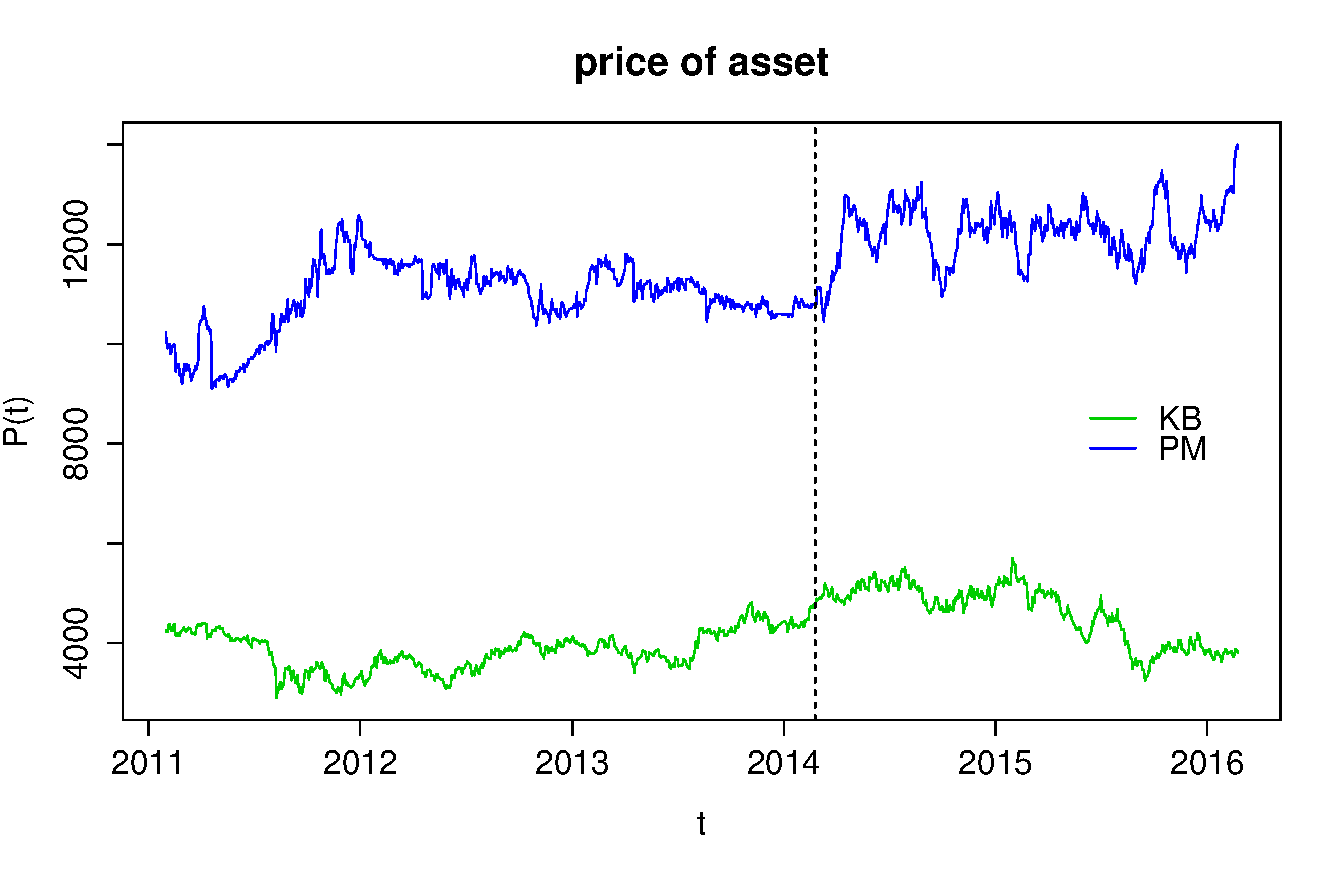
\includegraphics[width=13.5cm, clip, trim= 0 15 25 50]{IMG/ds_price_of_asset_KBPM_v2.pdf}	
  \caption{Model cen aktiv v portfoliu}  \label{price_of_asset}
\end{figure}

\begin{figure}[!htbp]
  \centering 
	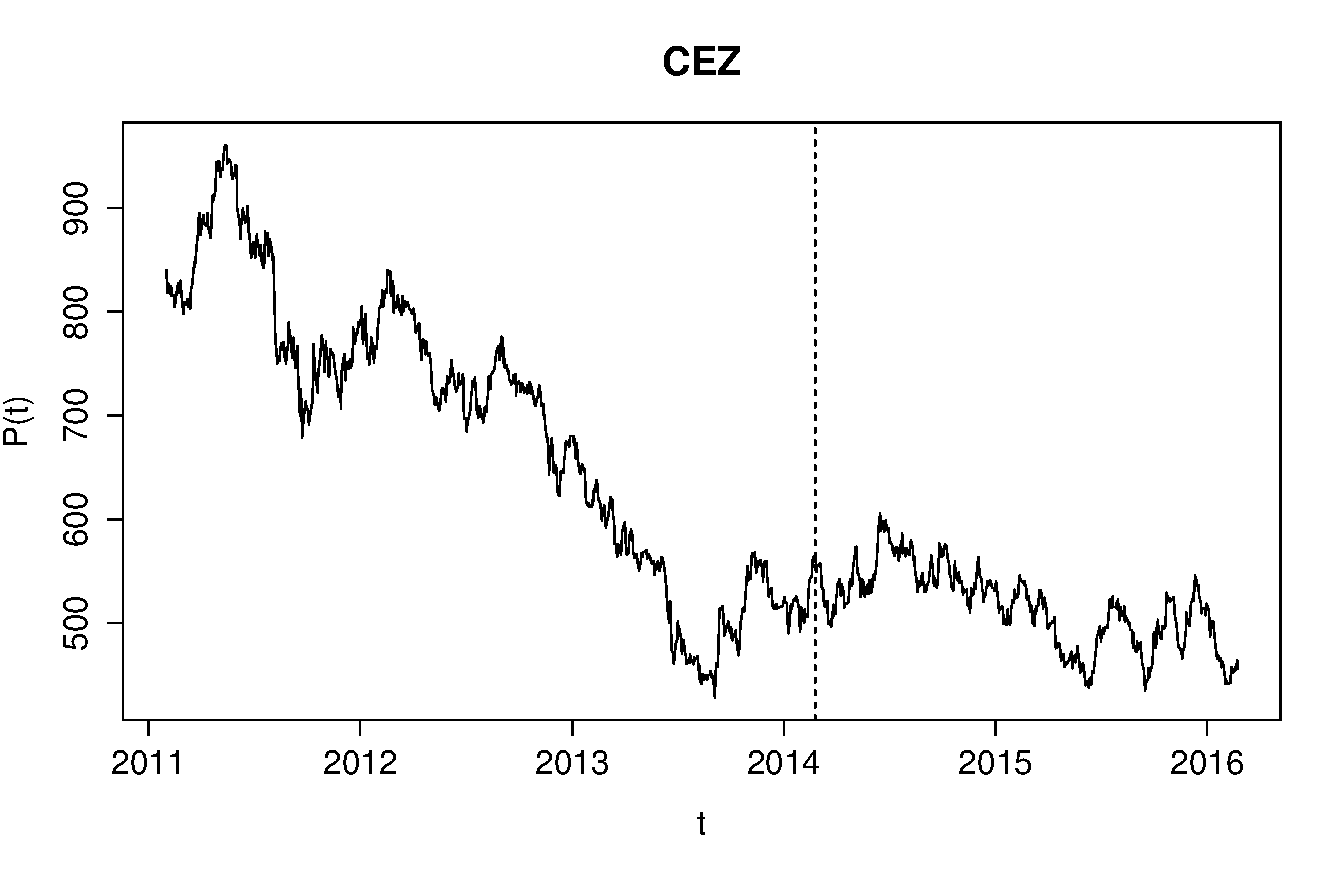
\includegraphics[width=6.6cm, clip, trim= 0 15 25 0]{IMG/ds_cez_v4.pdf}\quad
	\includegraphics[width=6.6cm, clip, trim= 0 15 25 0]{IMG/ds_o2_v4.pdf}\\	
	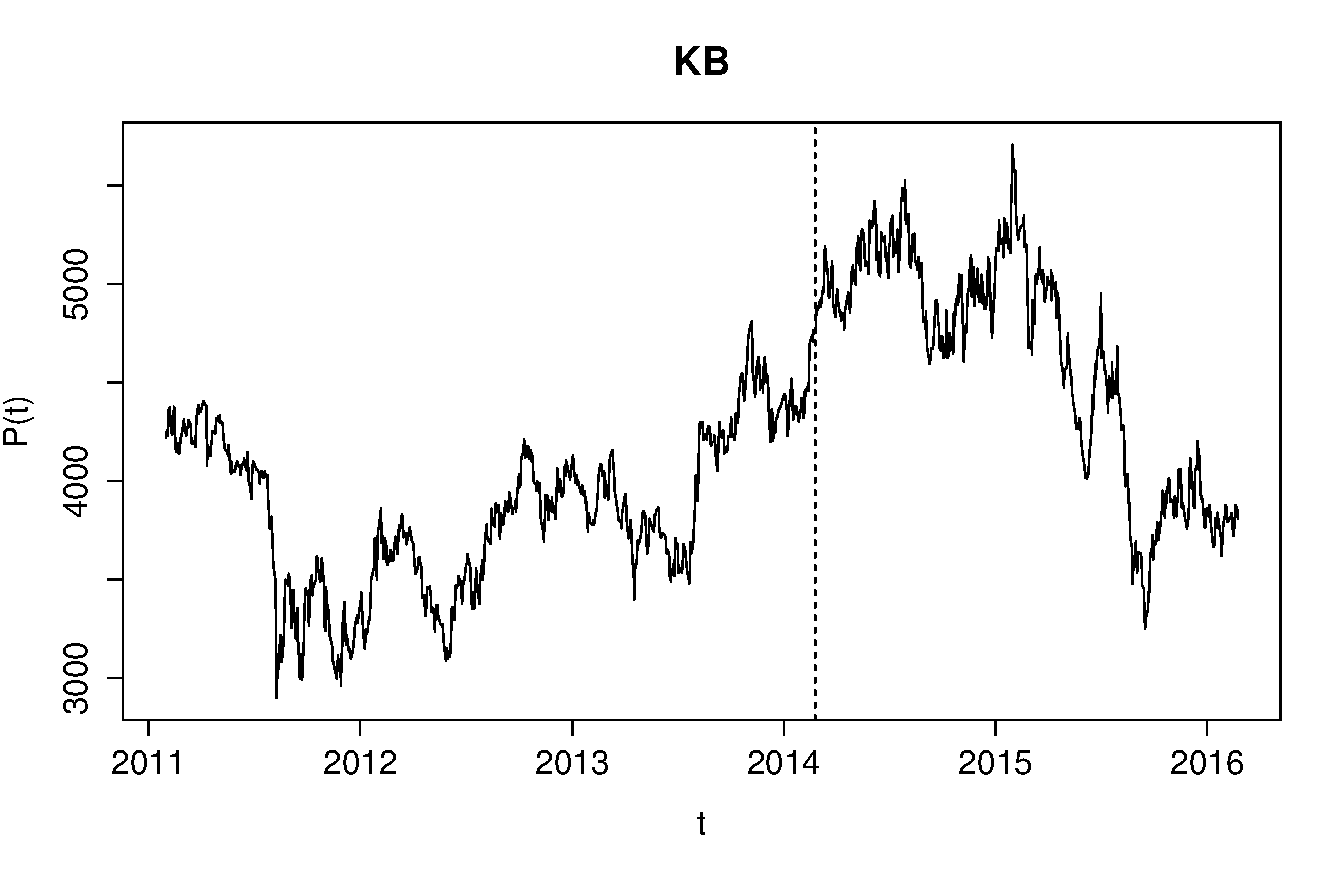
\includegraphics[width=6.6cm, clip, trim= 0 15 25 0]{IMG/ds_KB_v4.pdf}\quad
	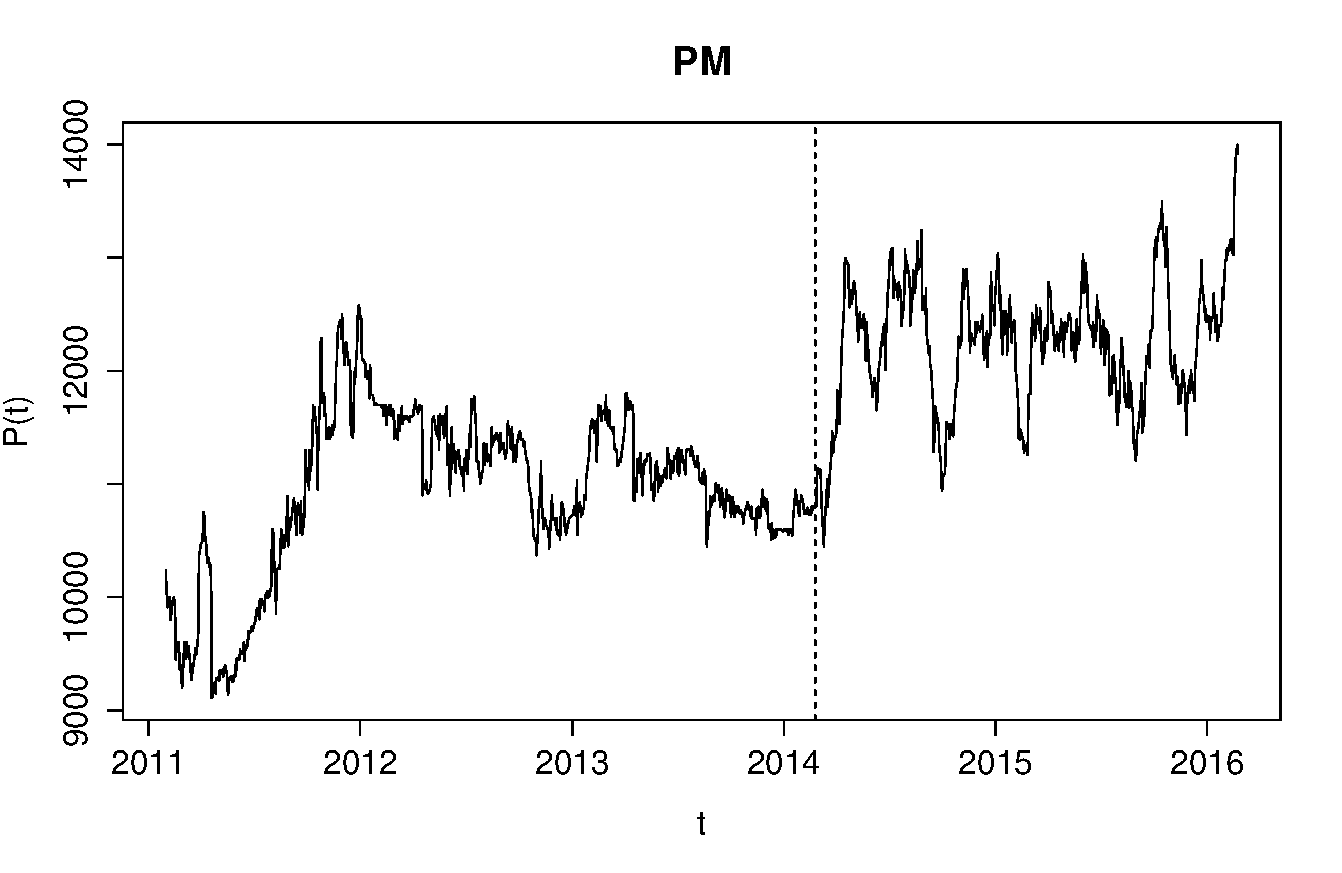
\includegraphics[width=6.6cm, clip, trim= 0 15 25 0]{IMG/ds_PM_v4.pdf}\\	
	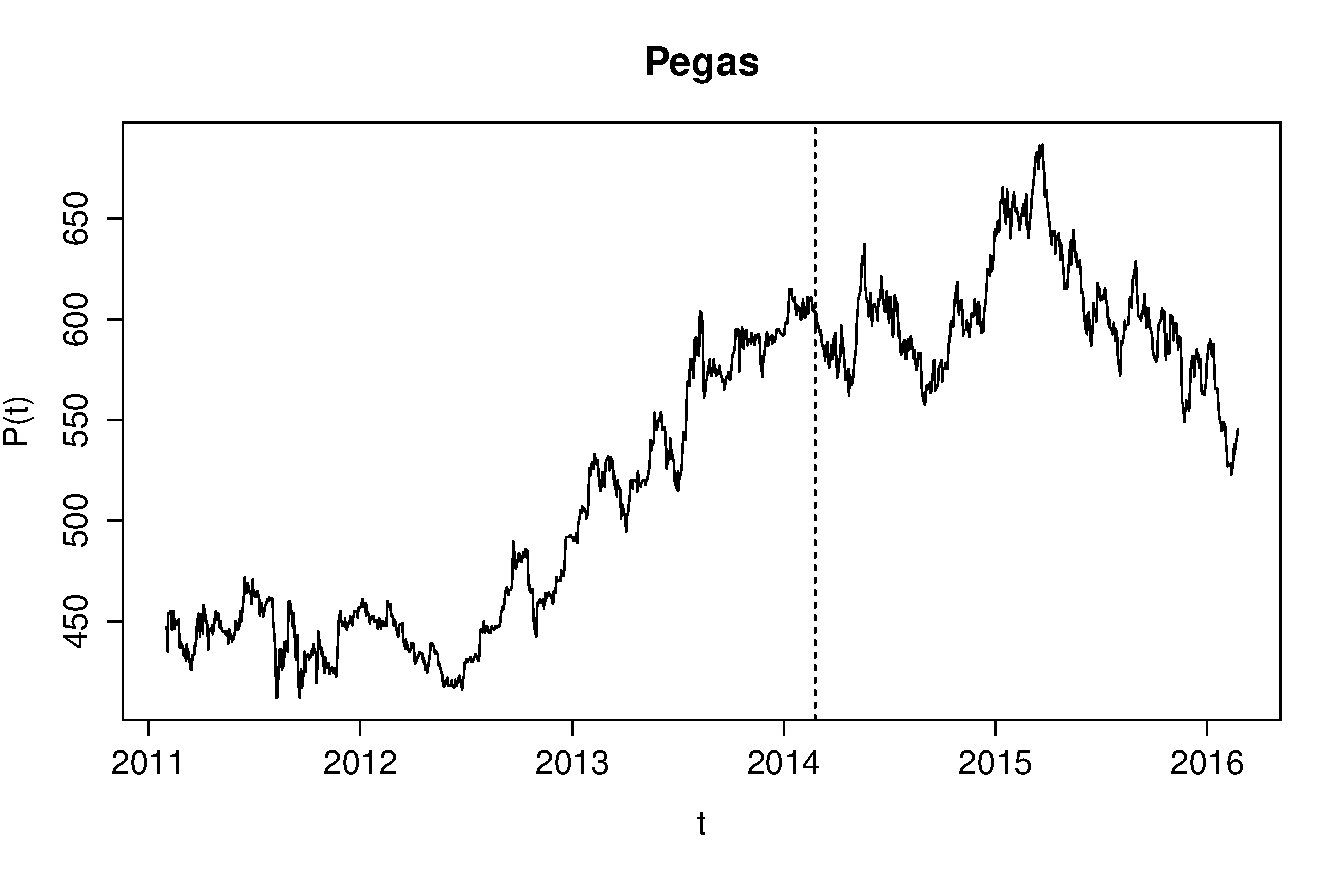
\includegraphics[width=6.6cm, clip, trim= 0 15 25 0]{IMG/ds_Pegas_v4.pdf}\quad
	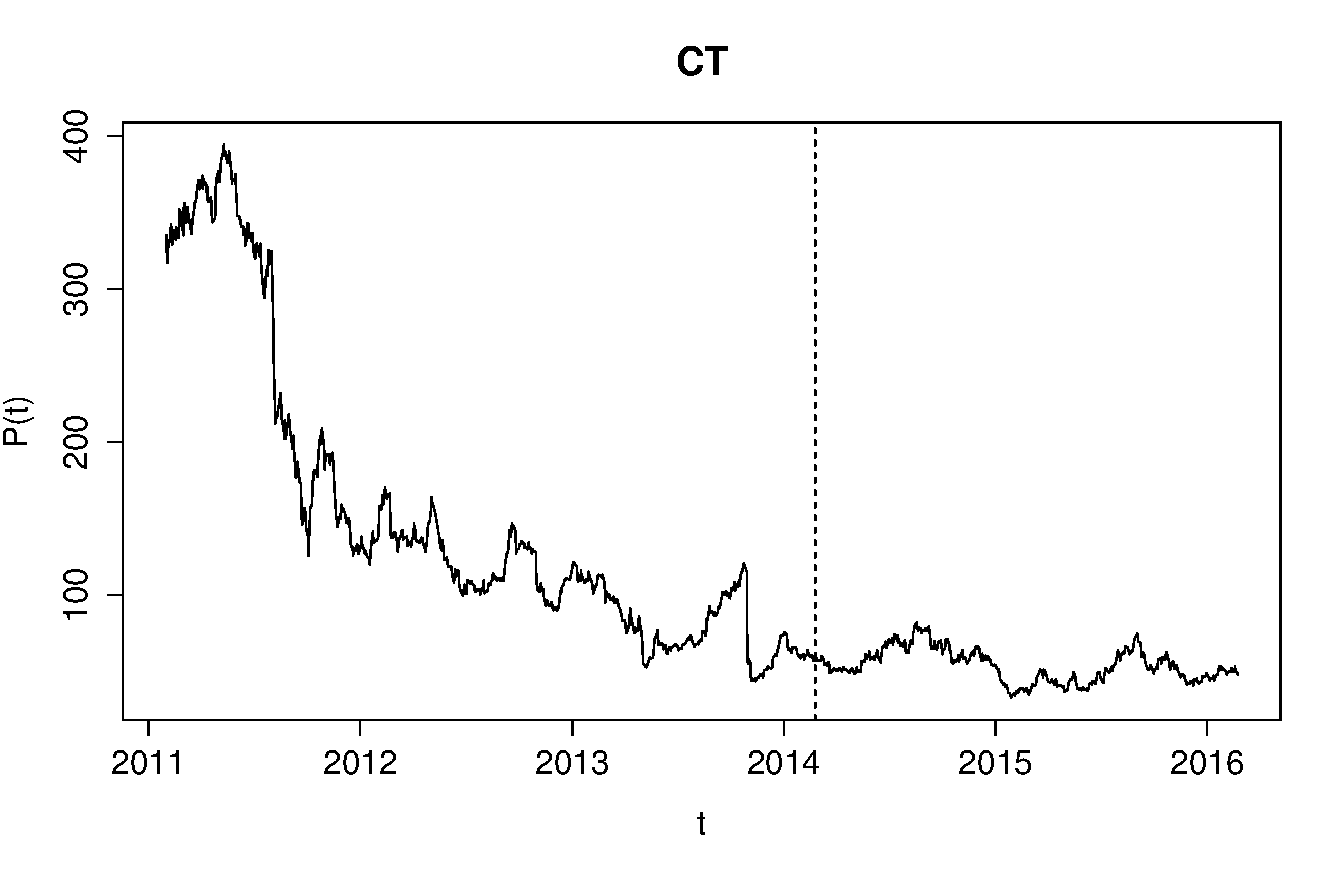
\includegraphics[width=6.6cm, clip, trim= 0 15 25 0]{IMG/ds_ct_v4.pdf}\\
	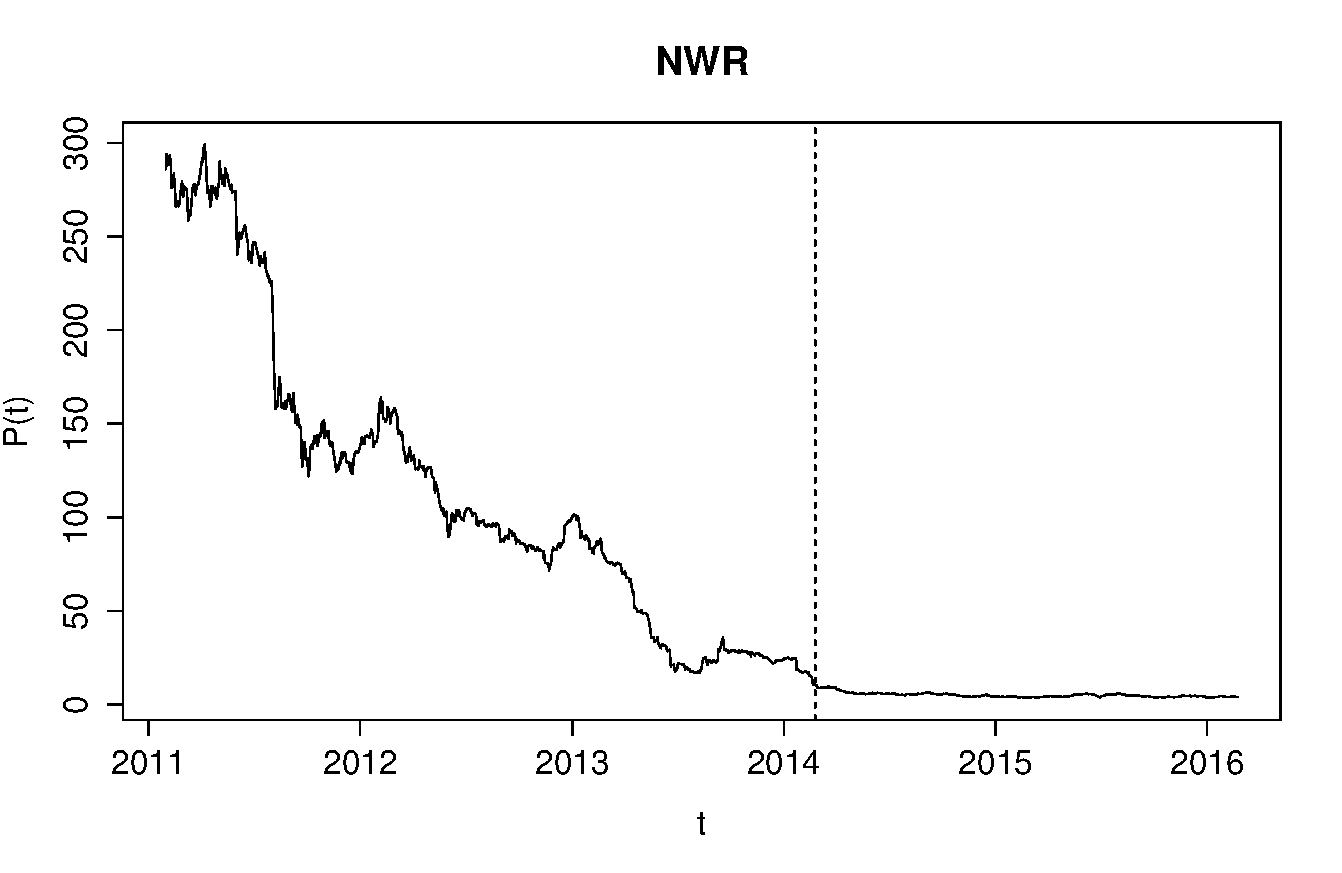
\includegraphics[width=6.6cm, clip, trim= 0 15 25 0]{IMG/ds_nwr_v4.pdf}	
  \caption{Model cen aktiv v portfoliu}  \label{price_of_asset}
\end{figure}

\begin{figure}[!htbp]
  \centering 
	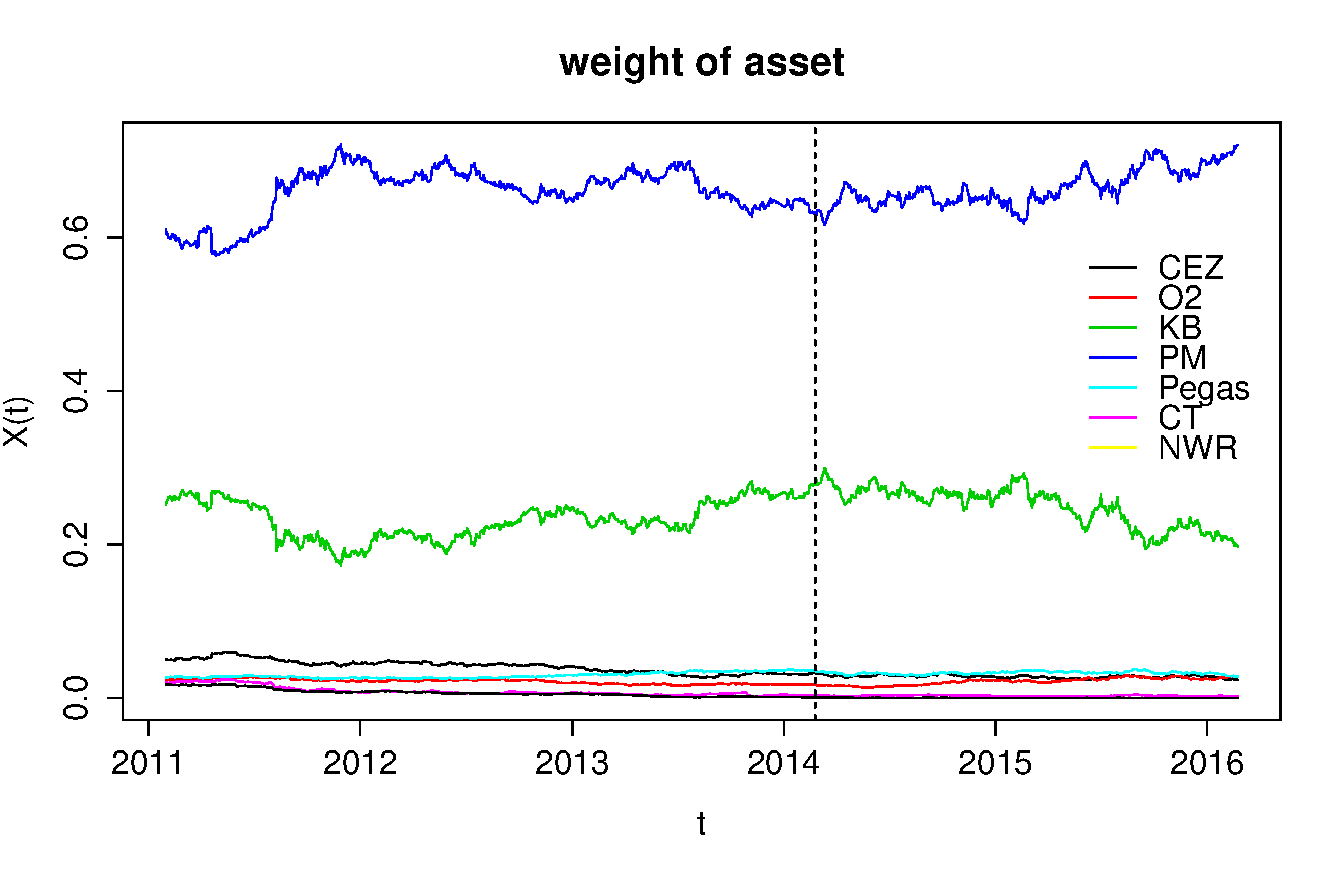
\includegraphics[width=13.5cm, clip, trim= 0 15 25 50]{IMG/ds_weight_of_asset_v5.pdf}
  \caption{Model vah aktiv v portfoliu}  \label{weight_of_asset}
\end{figure}

\begin{figure}[!htbp]
  \centering 
	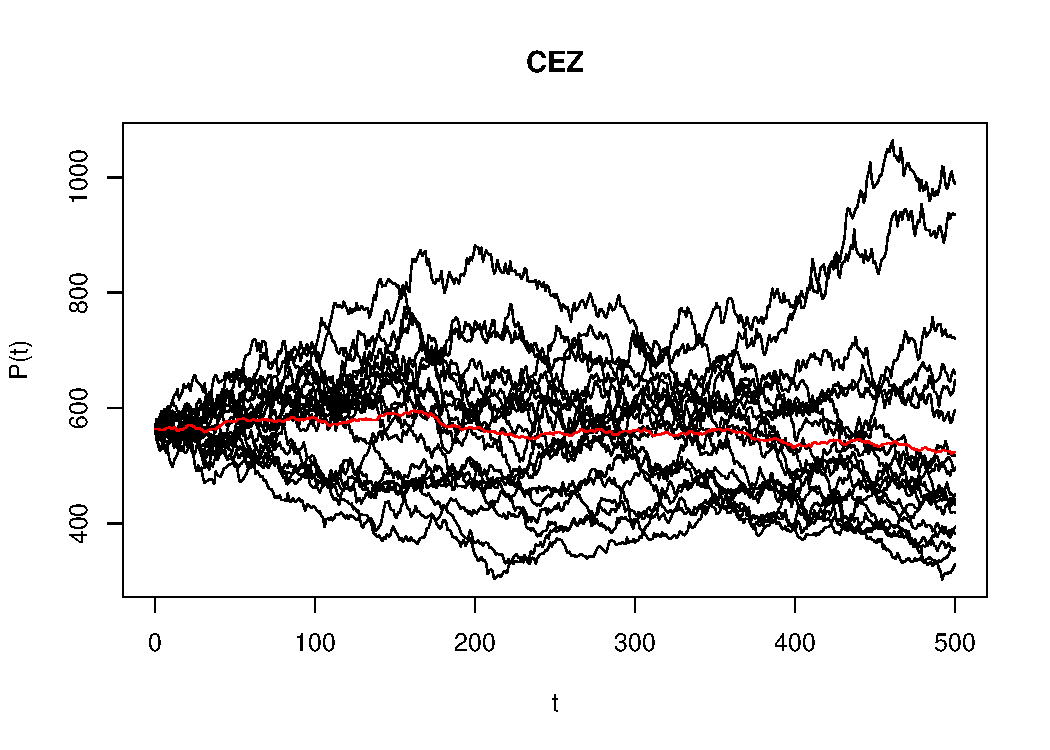
\includegraphics[width=13.5cm, clip, trim= 0 15 25 50]{IMG/avg_CEZ_v1.pdf}
  \caption{Dvacet simulací trajektorie stochastického procesu ceny akcií (společnost ČEZ) a jejich střední hodnota}  \label{avg_trajektorie}
\end{figure}

\begin{figure}[!htbp]
  \centering 
	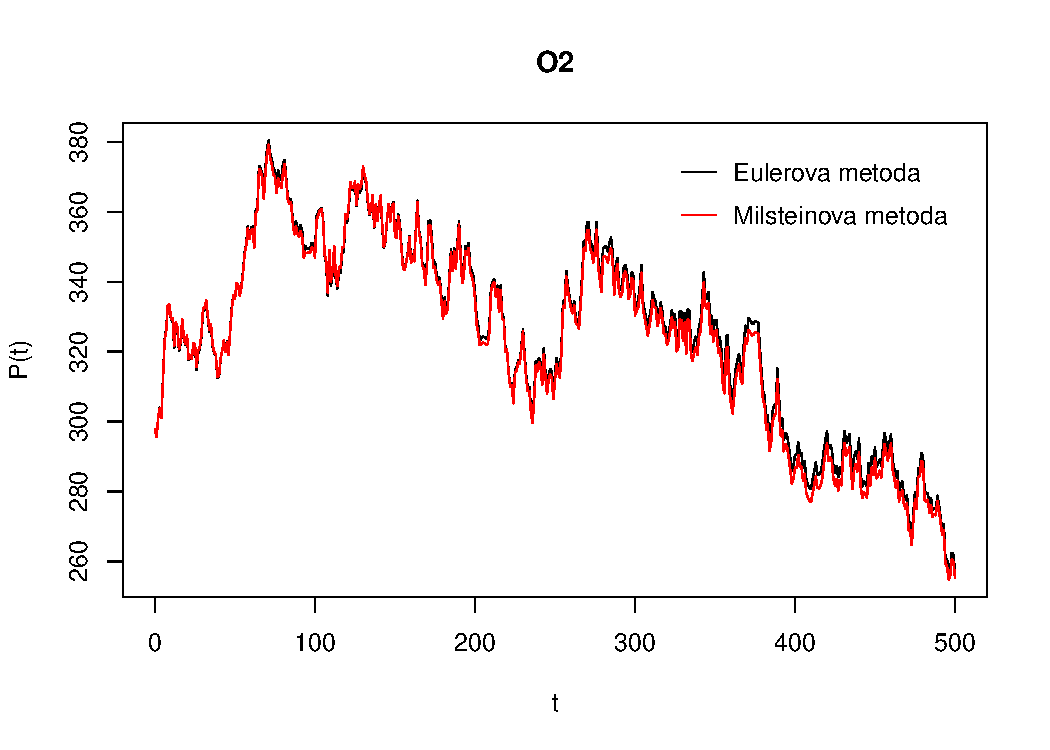
\includegraphics[width=13.5cm, clip, trim= 0 15 25 50]{IMG/e_m_o2_v2.pdf}
  \caption{Srovnání Eulerovy numerické metody a Milsteinovy numerické metody pro simulace trajektorií stochastického procesu ceny akcií (společnost O2)}  \label{euler_milstein}
\end{figure}

\begin{figure}[!htbp]
  \centering 
	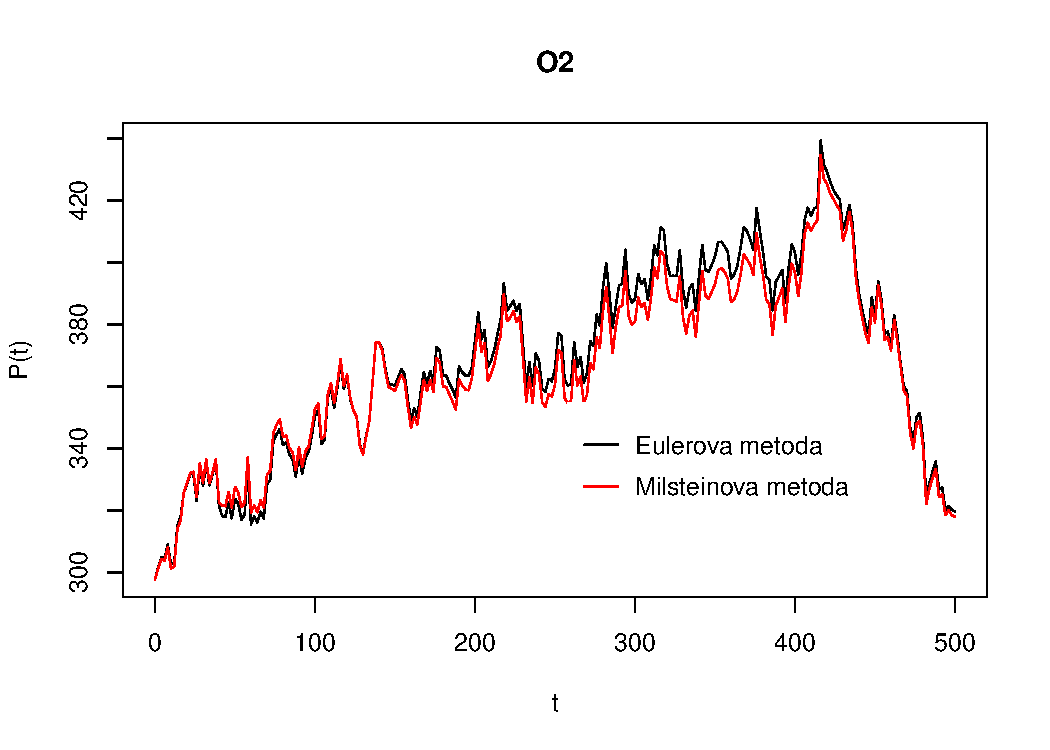
\includegraphics[width=6.6cm, clip, trim= 0 15 25 50]{IMG/e_m_o2_v3_q0_5.pdf}\quad
	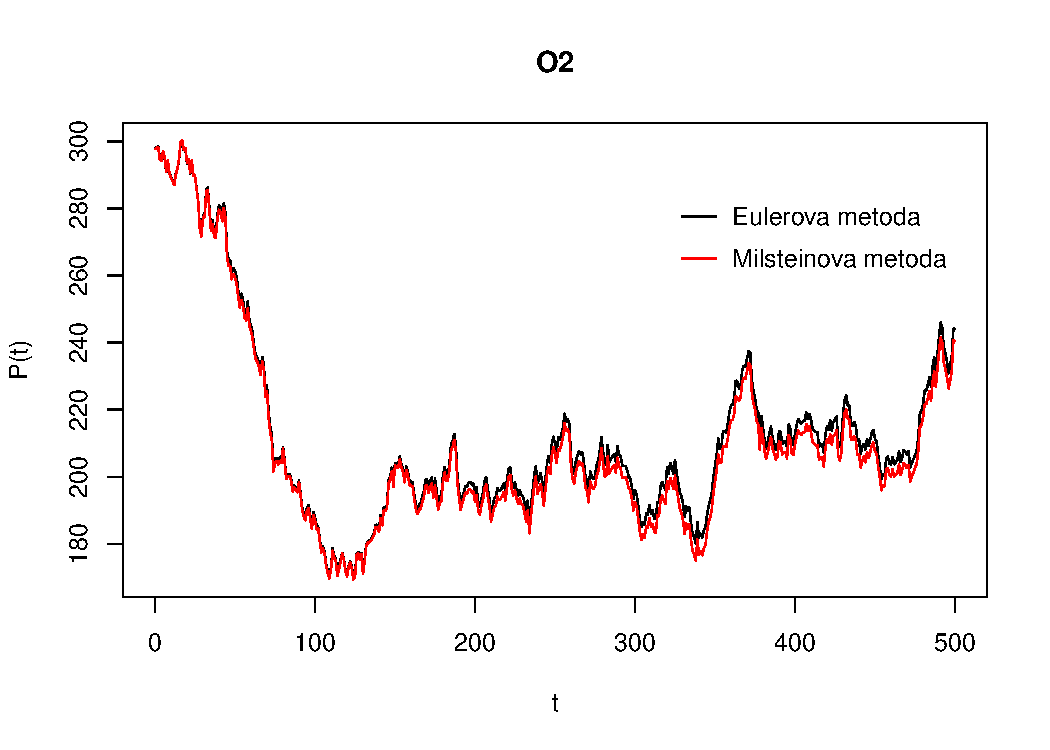
\includegraphics[width=6.6cm, clip, trim= 0 15 25 50]{IMG/e_m_o2_v3_q1.pdf}\\
	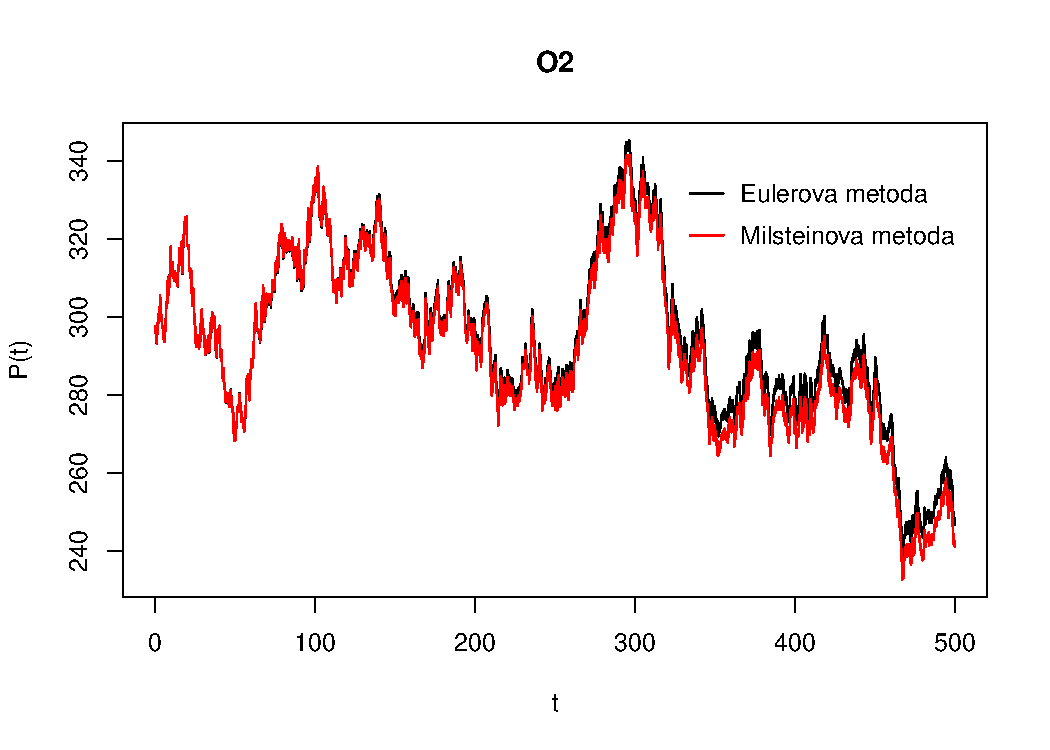
\includegraphics[width=6.6cm, clip, trim= 0 15 25 50]{IMG/e_m_o2_v3_q5.pdf}\quad
	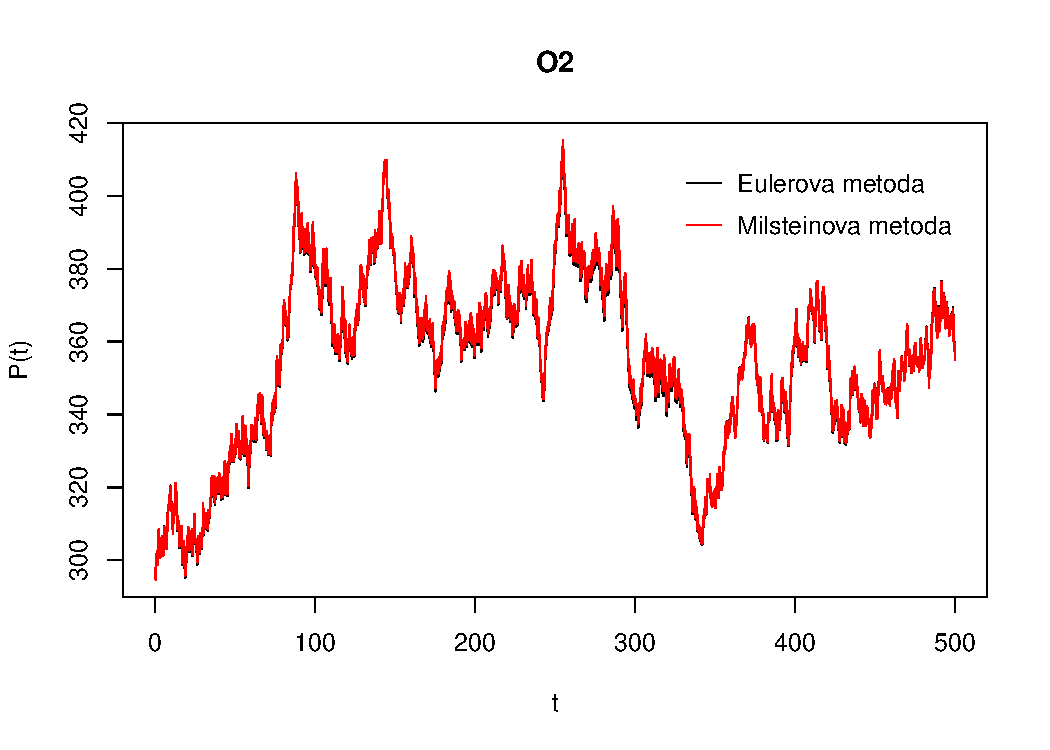
\includegraphics[width=6.6cm, clip, trim= 0 15 25 50]{IMG/e_m_o2_v3_q10.pdf}\\
	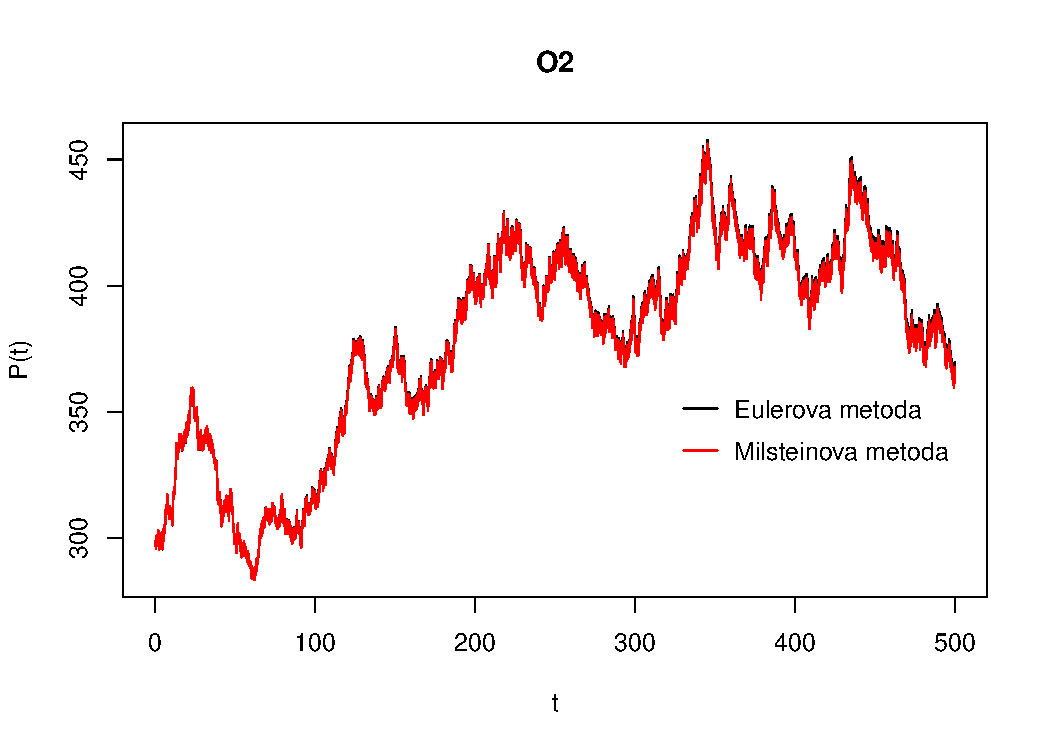
\includegraphics[width=6.6cm, clip, trim= 0 15 25 50]{IMG/e_m_o2_v3_q50.pdf}
  \caption{Srovnání Eulerovy numerické metody a Milsteinovy numerické metody pro simulace trajektorií stochastického procesu ceny akcií (společnost O2) s různými časovými kroky $\Delta_n\in\{2; 1; 0,2; 0,1; 0,02\}$}  \label{euler_milstein_q}
\end{figure}

%%%%%%%%%%%%%%%%%%{Credit Valuation Adjustment}
\begin{comment}
\chapter{Credit Valuation Adjustment}

Nedílnou součástí řízení banky je řízení bankovních rizik.
Obzvláště v poslední době se práce risk managementu dostává do popředí zájmu
a jsou patrné tendence ke sjednocování bankovní regulace na mezinárodní úrovni.
Důkazem spolupráce mezi institucemi bankovního dohledu je i vznik Basilejského výboru pro bankovní dohled.
Výbor vydává regulační standardy, doporučuje konkrétní postupy v oblasti bankovního dohledu a snaží se o sbližování regulačních norem. 
Řada států jeho doporučení zohledňuje a přijímá do vlastní legislativy a Česká republika v tomto není výjimkou.
Standardy vydávané výborem se označují Basel a byly dosud vydávány ve třech generacích označovaných jako Basel I, Basel II a Basel III. 
Vyjadřují kapitálové požadavky, zabývají se pravidly obezřetného podnikání bank a aktivitami bankovního dohledu.

Během celosvětové finanční krize, která odstartovala v roce 2008, se ukázala důležitost správného měření a řízení kreditního rizika protistrany (CCR) pro stabilitu finančního systému.
Kapitál pro kreditní riziko protistrany byl vyžadován již v Basel I.  
V reakci na finanční krizi Basel III představil nejen další požadavky pro výpočet kapitálu pro CCR, ale nově
předepisuje kapitálový požadavek pro riziko Credit Valuation Adjustment (CVA). 

CVA lze interpretovat jako úpravu tržní hodnoty derivátu o kreditní riziko protistrany.
Riziko CVA vyplývá jak z rizika změny pravděpodobnosti selhání protistrany tak změny tržních faktorů, které ovlivňují hodnotu derivátů.

Hlavním zdrojem informací pro vznik této kapitoly byla kniha Jona Gregoryho \cite{gregory2010},
články \cite{zhu2007} a \cite{pykhtin2010} a publikace \cite{brigo2014}.
Pěkný přehledový článek na toto téma vyšel v roce 2012 v Journal of Financial Economics \cite{arora2012}.
Zajímavý článek zabývající se zahrnutím Wrong-Way rizika do Monte Carlo simulace při výpočtu CVA publikovali John Hull a Alan White \cite{hull2012cva}.


%Analýza vzájemné vazby mezi rizikem a výnosy.

\section{Finanční rizika}
V následujícím textu seznámíme čtenáře s problematikou řízení finančních rizik, především úvěrového rizika.
Komplexní přehled o finančních rizicích poskytuje publikace  jednoho z nejznámějších českých ekonomů profesora Josefa Jílka \cite{jilek2000}.
Kniha zevrubně popisuje úvěrová, tržní a další finanční rizika a objasňuje podstatu, měření, řízení a regulace finančních rizik včetně použití derivátů.

Bankovní podnikání ohrožuje celá řada rizik, která obecně chápeme jako nebezpečí vzniku škody. 
Řídit tato rizika mimo jiné znamená odhadovat pravděpodobnost jejich vzniku a navrhovat metody k jejich snížení.
Banka je ohrožena nejen podnikatelskými riziky, ale také riziky finančními, které souvisí s její potenciální finanční ztrátou. 
Na tato rizika je soustředěna mimořádná pozornost odborné veřejnosti, bankovního dohledu, ale i samotného představenstva banky, jelikož řízení rizik má vliv na budoucí strategii podnikání banky.

Základním finančním rizikem je kreditní (též úvěrové) riziko.
Jedná se o riziko vyplývající z neschopnosti nebo neochoty protistrany splatit své závazky podle podmínek
kontraktu, což způsobí držiteli pohledávky ztrátu.
Jeho řízení má rozhodující význam pro úspěch nebo neúspěch nejen finančních institucí. 

Mezi významná bankovní rizika patří tržní riziko. 
Jedná se o riziko ztráty v souvislosti s pohybem tržních cen v důsledku nepříznivých změn tržních podmínek. 
Je zaměřeno na faktory, které mají vliv na finanční trh jako celek (nikoliv pouze na cenu jednotlivého aktiva).
Jeho význam vzrůstá s rostoucí angažovaností bank na finančních trzích. 

Úvěrové riziko a tržní riziko není možno od sebe zcela oddělovat.
Obě tato rizika v sobě spojuje kreditní riziko protistrany, jehož modelování je nedílnou součástí výpočtu Credit Valuation Adjustment. 

Dalšími finančními riziky jsou operační riziko a riziko likvidity.
Basel II %(International Convergence of Capital Measurement and Capital Standards) 
definoval operační riziko jako riziko ztráty vyplývající z nedostatků či selhání vnitřních procesů, osob a systémů nebo vlivem vnějších událostí.
Řízení operačního rizika slouží k zajištění provozní efektivity, snížení nákladů a zvýšení konkurenceschopnost.
Regulatorní orgány vymezují obezřetnostní požadavky na operační riziko.
Riziko likvidity je %riziko, že banka ztratí schopnost dostát svým finančním závazkům v době, kdy se stanou splatnými (bez toho aby došlo k narušení běžných činností nebo finanční kondice banky) nebo nebude moci snadno (v požadovaném čase a za obvyklou cenu) uzavřít pozici na trhu z důvodu nedostatečné hloubky nebo narušení trhu.
riziko ztráty schopnosti dostát finančním závazkům v době, kdy se stanou splatnými, nebo riziko ztráty schopnosti financovat aktiva.
Princip řízení rizika likvidity zahrnuje alokaci aktiv a pasiv do časových košů a následné určování likvidního gapu v jednotlivých časových koších. 
Těmito dvěma finančními riziky se v této práci nebudeme dále podrobněji zabývat.

\subsection{Kreditní riziko protistrany}
Counterparty Credit Risk (CCR), v překladu \textit{kreditní riziko protistrany},  představuje možnost, že banka utrpí ztrátu z derivátového obchodu nebo při financování aktiva, která bude způsobena selháním protistrany transakce. 
Riziko selhání (defaultu) představuje základní rizikovou složkou kreditního rizika a jeho parametrem je pravděpodobnost neplnění. 
Definice tohoto jevu není zcela jednoznačná, většinou se však chápe jako stav finanční tísně, bránící ve splnění závazku.

Riziko protistrany závisí na spolehlivosti obchodního partnera, ať už se jedná o emitenta, který vydává, nabízí a prodává investiční produkt a zavazuje se k jeho splacení (resp. vyrovnání s ním spojených závazků), nebo finančního zprostředkovatele, kterému jsou svěřeny prostředky buď do správy, nebo k provedení investiční transakce.

Existují specializované společnosti nazývané ratingové agentury, které se zabývají hodnocením rizik emitentů %(států, veřejně obchodovaných společností finančních i nefinančních, soukromých firem, měst, regionálních celků apod.) 
a na jeho základě jim udělují kód vyjadřující bonitu či důvěryhodnost, tzv. \textit{rating}.
Pro investory je rating spolehlivou informací o kreditním riziku emitenta příslušného finančního instrumentu, případně finančního zprostředkovatele. 
Nejznámějšími ratingovými agenturami jsou Moody's, Standard \& Poor's a Fitch. Každá z těchto agentur má vlastní hodnotící stupnici a zvyklosti.

Obecně se ratingové stupnice dělí na dvě části -- investiční pásmo a spekulativní pásmo.
Ratingy z investičního pásma přiznávají ratingové agentury finanční instrumentům, do kterých doporučují investovat. Pod touto úrovní leží pásmo spekulativních investic, u kterých je očekáváno značné riziko ztráty.

Typickým představitelem emitenta s velmi nízkým rizikem je vláda vyspělého státu, která vydává dluhopisy, jež jsou chápány jako bezrizikové  investiční instrumenty. Nízké kreditní riziko mohou mít i velké tuzemské či mezinárodními společnosti s dobrými hospodářskými výsledky, zejména pokud mají (dle všeobecného názoru) schopný management, což vede k předpokladu dobrých výsledků a udržení pozice na trhu i v budoucnosti.
Rating je využíván také k posouzení  důvěryhodnosti finančního partnera, který danou finanční investici zprostředkovává.

Důležitým faktem při výpočtu kapitálového požadavku pro CCR je  bilaterální charakter tohoto rizika. Což znamená, že kreditním rizikem protistrany jsou zatíženy obě strany obchodu.

Velmi dobrý úvod do problematiky řízení rizika protistrany poskytuje článek \cite{canabarro2003measuring} autorů Eduarda Canabarra, vedoucího oddělení řízení rizika v bankovní společnosti Goldman Sachs, a profesora Stanfordské univerzity Darrella Duffieho.

%\section{Úvěrová úprava v ocenění finančních derivátů}
\section{Koncept CVA}
V rámci překladu termínu \textit{Credit Valuation Adjustment (CVA)}  se můžeme setkat s více možnostmi.
Například Česká národní banka používá výraz \textit{úprava úvěrového ocenění}.
V jiných textech nalezneme pojem  \textit{kreditní přirážka k tržnímu ocenění} nebo \textit{úvěrová úprava v ocenění finančních derivátů}.
Z důvodu přehlednosti budeme v textu této práce používat především zkratku CVA nebo anglický termín.

\subsection{Expozice protistrany}
\textit{Expozici protistrany} v čase $t$ značíme $E(t)$ a definujeme jako celkovou výši nesplacených pohledávek danou protistranou.
%Expozice kvantifikuje potenciální ekonomickou ztrátu v případě selhání protistrany.
Hodnota expozice protistrany kvantifikuje do jaké míry je věřitel vystaven riziku ztráty v případě neplnění dlužníka.

Uvažujme portfolio $N$ derivátových obchodů banky s danou protistranou.
Splatnost kontraktu s nejdelší splatností v tomto portfoliu označíme $T$. 
Nechť $\tau$ je náhodná veličina, která označuje čas selhání dané protistrany a má známou distribuční funkci $P(t)=\Pr(\tau\leq t)$.

Budeme zkoumat hodnotu portfolia z pohledu banky.
Expozice protistrany $E(t)$ v čase $t$ je dána hodnotami derivátových odchodů s danou protistranou v čase $t$.
Hodnotu $i$-tého derivátu z portfolia v čase $t$  označíme $V_i(t)$.
Pak hodnota portfolia v čase $t$ je definována jako
\begin{equation}
V(t)=\sum_{i=1}^N V_i(t).
\end{equation}
V případě, že banka nemá s protistranou uzavřenou dohodu o vzájemném započítávání pohledávek a závazků (tzn. netting), expozice protistrany $E(t)$ je 
\begin{equation}
E(t)=\sum_{i=1}^N\max\{V_i(t),0\}.
\end{equation}
Pokud banka s protistranou uzavře smlouvu o nettingu, pak je expozice dána jako
\begin{equation}
E(t)=\max\{V(t),0\}.
\end{equation}
Využívání nettingu slouží ke snížení úvěrového a tržního rizika. 
Při použití nettingu je expozice protistrany menší nebo rovna expozici v případě, kdy netting neuvažujeme. 

Další možnost jak snížit expozici je zajištění.
Banka uzavírá s protistranou dohodu o výzvě k doplnění zajištění (margin call).
Protistrana pak musí poskytnout bance zajištění vždy, když hodnota portfolia překročí určenou mez.
Naopak pokud hodnota portfolia klesne pod tuto mez, banka zajištění opět vrátí.
Expozice protistrany, která zohledňuje zajištění se určí jako
\begin{equation}
E(t)=\max\{V(t)-C(t),0\},
\end{equation}
kde $C(t)$ je hodnota zajištění (které banka přijala) v čase $t$.  

\subsection{diskontovani}
Výpočet dnešní hodnoty při tržní úrokové míře
Diskontování je matematický postup, kdy jsou přepočítány (diskontovány) budoucí výnosy na současnou hodnotu investice s použitím diskontní míry.
Diskontní míra je procentní sazba, kterou se diskontuje budoucí hodnota na současnou hodnotu.

Diskontovaná hodnota je současná hodnota. Je to jedna z metod hodnocení investic, kdy se budoucí výnosy převádějí na hodnotu, kterou by měly dnes.
Diskontování je postup, kdy jsou přepočteny (diskontovány) budoucí výnosy v jednotlivých obdobích na současnou hodnotu a sečteny s použitím diskontní míry (obvyklá výnosová míra).

\subsection{Pravděpodobnost selhání}

Pravděpodobnost selhání (PD), Probability of Default, udává v procentech s jakou pravděpodobností dojde k selhání klienta během jednoho roku.

%\subsection{Modely zajištění}

%\section{Poznámky CVA}

%odhad parametrů – proces hledání hodnot parametrů, které vedou k co nejlepší shodě výsledků modelu s měřenými daty pomocí některé ze statistických metod 
%kalibrace – totéž jako odhad parametrů, ale ne nezbytně pomocí statistických metod


%Čím horší je bonita klienta .... viz GoogleDisk


\end{comment}
%%%%%%%%%%%%%%%%%%%%%%%%%%%%%%%


\nocite{}  %umisti do literatury i necitovanou polozku a \nocite{*} umisti do literatury vsechny polozky z bibtex databaze 

\cleardoublepage
\phantomsection 

\addcontentsline{toc}{chapter}{Literatura}
%\bibliographystyle{plain}
\bibliographystyle{abbrv}
\bibliography{bibliography}

%\cleardoublepage
%\phantomsection 
%\addcontentsline{toc}{chapter}{Příloha}

%\renewcommand{\thechapter}{\Alph{chapter}} %nový čítač kapitol, příkaz \Alph nastavuje, že čítačem budou velká písmena
%\setcounter{chapter}{0} %nastaví čítač kapitol na 0

\appendix %příkaz, který první číslo v názvu kapitoly nebo sekce mění na písmeno

%\nocite{976825, 979237, 979245, 1077842, 1093598, 1167343, 1167503, 1183811} %moje publikace

\chapter[Příloha -- Publikace autorky]{Příloha}
\section*{Publikace autorky}
%\bibliographystyle{abbrv}
%\bibliography{moje}
\begin{itemize}

\item[I.]
L.~Křivánková.
\newblock Equilibrium models for portfolio selection.
\newblock In M.~e. Jiří~Zelinka, editor, {\em Mathematical Models and
  Financial Mathematics. Book of short papers}, pages 35--42, Brno, 2014.
  Masaryk University.

\item[II.]
L.~Křivánková.
\newblock Asset-pricing models in portfolio theory.
\newblock In M.~e. Jiří~Zelinka, editor, {\em Financial Mathematics in
  Practice II, Book of short papers}, pages 42--49, Brno, 2013. Masaryk
  University.

\item[III.]
L.~Křivánková.
\newblock Continuous-time models in portfolio theory.
\newblock In {\em XX International Conference PDMU-2012 Problems of Decision
  Making under Uncertainties}, pages 95--104, Brno, 2012. University of
  Defence.

\item[IV.]
L.~Křivánková.
\newblock The black-scholes equation for barrier options.
\newblock In {\em 7. konference o matematice a fyzice na vysokých školách
  technických s mezinárodní účastí : Sborník příspěvků část 1 -
  matematika}, 2011.

\item[V.]
L.~Křivánková.
\newblock Wiener process and applications.
\newblock In {\em Workshop of the Jaroslav Hájek Center, Book of short
  papers}, 2010.

\item[VI.]
S.~Kafková and L.~Křivánková.
\newblock Generalized linear models in vehicle insurance.
\newblock {\em Acta Universitatis Agriculturae et Silviculturae Mendelianae
  Brunensis}, 62, 2014.

\item[VII.]
S.~Kafková, L.~Křivánková, and M.~Leváková.
\newblock Survival analysis of patients with brain tumour.
\newblock In M.~e. Jiří~Zelinka, editor, {\em Mathematical Models and
  Financial Mathematics. Book of short papers}, pages 27--33, Brno, 2014.
  Masaryk University.

\end{itemize}


\chapter[Příloha -- Ukázka datového souboru]{Příloha}
\section*{Ukázka datového souboru}
V příloze je uvedena ukázka datového souboru analyzovaného v Kapitole \ref{muj_model}.
\begin{figure}[!htbp]
  \centering 
	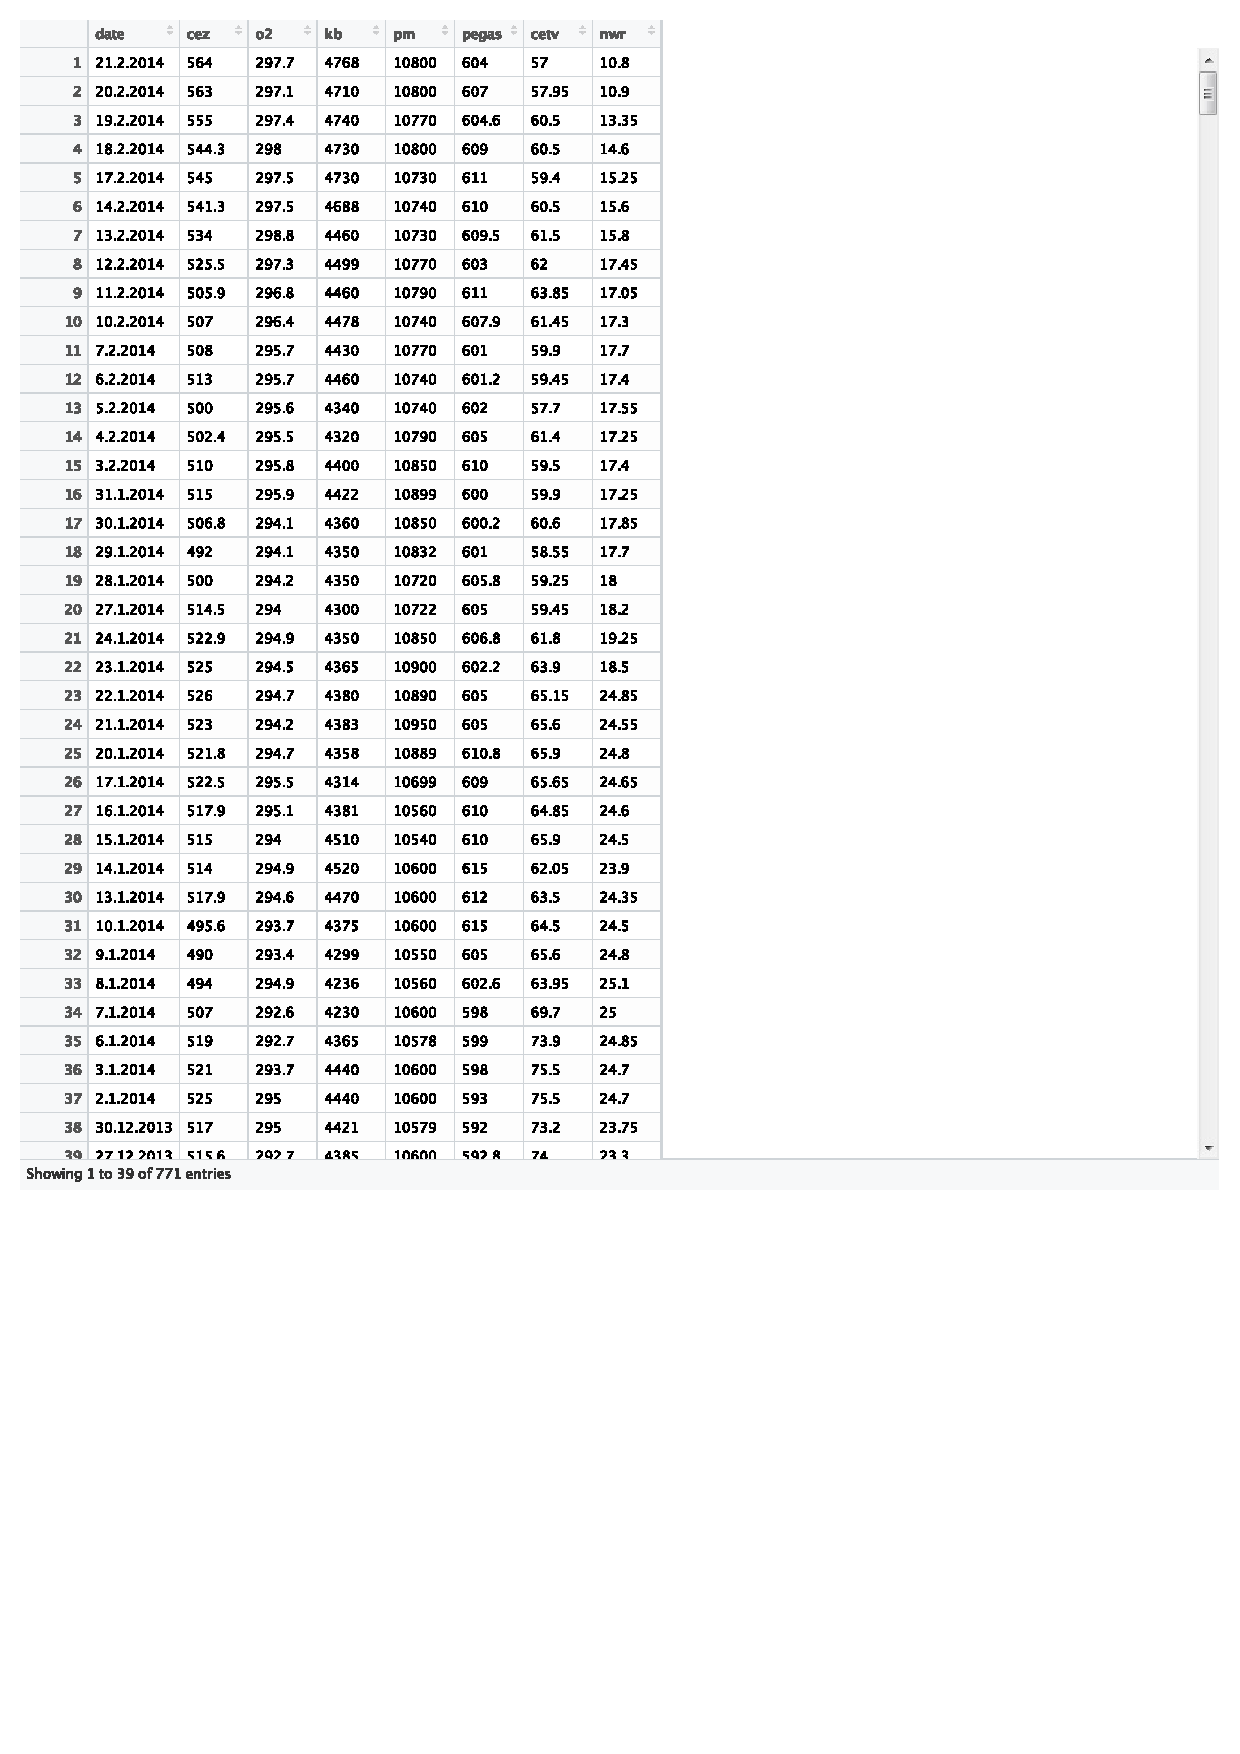
\includegraphics[width=13.5cm, clip, trim= 0 270 0 10]{IMG/data.pdf}
%  \caption{}  %\label{}
\end{figure}
\end{document}


% Synonyma:
%
% článek, text, publikace, monografie, kniha
% definovat, zformulovat
% jev, fenomén
% popisovat, charakterizovat, zachytit, vystihovat, postihovat, vyznačovat, určovat

%Užitečné příkazy:
%
%\linebreak